\documentclass[final,12pt]{colt2025} % Anonymized submission
%\documentclass[final,12pt]{colt2025} % Include author names

% The following packages will be automatically loaded:
% amsmath, amssymb, natbib, graphicx, url, algorithm2e

%
\setlength\unitlength{1mm}
\newcommand{\twodots}{\mathinner {\ldotp \ldotp}}
% bb font symbols
\newcommand{\Rho}{\mathrm{P}}
\newcommand{\Tau}{\mathrm{T}}

\newfont{\bbb}{msbm10 scaled 700}
\newcommand{\CCC}{\mbox{\bbb C}}

\newfont{\bb}{msbm10 scaled 1100}
\newcommand{\CC}{\mbox{\bb C}}
\newcommand{\PP}{\mbox{\bb P}}
\newcommand{\RR}{\mbox{\bb R}}
\newcommand{\QQ}{\mbox{\bb Q}}
\newcommand{\ZZ}{\mbox{\bb Z}}
\newcommand{\FF}{\mbox{\bb F}}
\newcommand{\GG}{\mbox{\bb G}}
\newcommand{\EE}{\mbox{\bb E}}
\newcommand{\NN}{\mbox{\bb N}}
\newcommand{\KK}{\mbox{\bb K}}
\newcommand{\HH}{\mbox{\bb H}}
\newcommand{\SSS}{\mbox{\bb S}}
\newcommand{\UU}{\mbox{\bb U}}
\newcommand{\VV}{\mbox{\bb V}}


\newcommand{\yy}{\mathbbm{y}}
\newcommand{\xx}{\mathbbm{x}}
\newcommand{\zz}{\mathbbm{z}}
\newcommand{\sss}{\mathbbm{s}}
\newcommand{\rr}{\mathbbm{r}}
\newcommand{\pp}{\mathbbm{p}}
\newcommand{\qq}{\mathbbm{q}}
\newcommand{\ww}{\mathbbm{w}}
\newcommand{\hh}{\mathbbm{h}}
\newcommand{\vvv}{\mathbbm{v}}

% Vectors

\newcommand{\av}{{\bf a}}
\newcommand{\bv}{{\bf b}}
\newcommand{\cv}{{\bf c}}
\newcommand{\dv}{{\bf d}}
\newcommand{\ev}{{\bf e}}
\newcommand{\fv}{{\bf f}}
\newcommand{\gv}{{\bf g}}
\newcommand{\hv}{{\bf h}}
\newcommand{\iv}{{\bf i}}
\newcommand{\jv}{{\bf j}}
\newcommand{\kv}{{\bf k}}
\newcommand{\lv}{{\bf l}}
\newcommand{\mv}{{\bf m}}
\newcommand{\nv}{{\bf n}}
\newcommand{\ov}{{\bf o}}
\newcommand{\pv}{{\bf p}}
\newcommand{\qv}{{\bf q}}
\newcommand{\rv}{{\bf r}}
\newcommand{\sv}{{\bf s}}
\newcommand{\tv}{{\bf t}}
\newcommand{\uv}{{\bf u}}
\newcommand{\wv}{{\bf w}}
\newcommand{\vv}{{\bf v}}
\newcommand{\xv}{{\bf x}}
\newcommand{\yv}{{\bf y}}
\newcommand{\zv}{{\bf z}}
\newcommand{\zerov}{{\bf 0}}
\newcommand{\onev}{{\bf 1}}

% Matrices

\newcommand{\Am}{{\bf A}}
\newcommand{\Bm}{{\bf B}}
\newcommand{\Cm}{{\bf C}}
\newcommand{\Dm}{{\bf D}}
\newcommand{\Em}{{\bf E}}
\newcommand{\Fm}{{\bf F}}
\newcommand{\Gm}{{\bf G}}
\newcommand{\Hm}{{\bf H}}
\newcommand{\Id}{{\bf I}}
\newcommand{\Jm}{{\bf J}}
\newcommand{\Km}{{\bf K}}
\newcommand{\Lm}{{\bf L}}
\newcommand{\Mm}{{\bf M}}
\newcommand{\Nm}{{\bf N}}
\newcommand{\Om}{{\bf O}}
\newcommand{\Pm}{{\bf P}}
\newcommand{\Qm}{{\bf Q}}
\newcommand{\Rm}{{\bf R}}
\newcommand{\Sm}{{\bf S}}
\newcommand{\Tm}{{\bf T}}
\newcommand{\Um}{{\bf U}}
\newcommand{\Wm}{{\bf W}}
\newcommand{\Vm}{{\bf V}}
\newcommand{\Xm}{{\bf X}}
\newcommand{\Ym}{{\bf Y}}
\newcommand{\Zm}{{\bf Z}}

% Calligraphic

\newcommand{\Ac}{{\cal A}}
\newcommand{\Bc}{{\cal B}}
\newcommand{\Cc}{{\cal C}}
\newcommand{\Dc}{{\cal D}}
\newcommand{\Ec}{{\cal E}}
\newcommand{\Fc}{{\cal F}}
\newcommand{\Gc}{{\cal G}}
\newcommand{\Hc}{{\cal H}}
\newcommand{\Ic}{{\cal I}}
\newcommand{\Jc}{{\cal J}}
\newcommand{\Kc}{{\cal K}}
\newcommand{\Lc}{{\cal L}}
\newcommand{\Mc}{{\cal M}}
\newcommand{\Nc}{{\cal N}}
\newcommand{\nc}{{\cal n}}
\newcommand{\Oc}{{\cal O}}
\newcommand{\Pc}{{\cal P}}
\newcommand{\Qc}{{\cal Q}}
\newcommand{\Rc}{{\cal R}}
\newcommand{\Sc}{{\cal S}}
\newcommand{\Tc}{{\cal T}}
\newcommand{\Uc}{{\cal U}}
\newcommand{\Wc}{{\cal W}}
\newcommand{\Vc}{{\cal V}}
\newcommand{\Xc}{{\cal X}}
\newcommand{\Yc}{{\cal Y}}
\newcommand{\Zc}{{\cal Z}}

% Bold greek letters

\newcommand{\alphav}{\hbox{\boldmath$\alpha$}}
\newcommand{\betav}{\hbox{\boldmath$\beta$}}
\newcommand{\gammav}{\hbox{\boldmath$\gamma$}}
\newcommand{\deltav}{\hbox{\boldmath$\delta$}}
\newcommand{\etav}{\hbox{\boldmath$\eta$}}
\newcommand{\lambdav}{\hbox{\boldmath$\lambda$}}
\newcommand{\epsilonv}{\hbox{\boldmath$\epsilon$}}
\newcommand{\nuv}{\hbox{\boldmath$\nu$}}
\newcommand{\muv}{\hbox{\boldmath$\mu$}}
\newcommand{\zetav}{\hbox{\boldmath$\zeta$}}
\newcommand{\phiv}{\hbox{\boldmath$\phi$}}
\newcommand{\psiv}{\hbox{\boldmath$\psi$}}
\newcommand{\thetav}{\hbox{\boldmath$\theta$}}
\newcommand{\tauv}{\hbox{\boldmath$\tau$}}
\newcommand{\omegav}{\hbox{\boldmath$\omega$}}
\newcommand{\xiv}{\hbox{\boldmath$\xi$}}
\newcommand{\sigmav}{\hbox{\boldmath$\sigma$}}
\newcommand{\piv}{\hbox{\boldmath$\pi$}}
\newcommand{\rhov}{\hbox{\boldmath$\rho$}}
\newcommand{\upsilonv}{\hbox{\boldmath$\upsilon$}}

\newcommand{\Gammam}{\hbox{\boldmath$\Gamma$}}
\newcommand{\Lambdam}{\hbox{\boldmath$\Lambda$}}
\newcommand{\Deltam}{\hbox{\boldmath$\Delta$}}
\newcommand{\Sigmam}{\hbox{\boldmath$\Sigma$}}
\newcommand{\Phim}{\hbox{\boldmath$\Phi$}}
\newcommand{\Pim}{\hbox{\boldmath$\Pi$}}
\newcommand{\Psim}{\hbox{\boldmath$\Psi$}}
\newcommand{\Thetam}{\hbox{\boldmath$\Theta$}}
\newcommand{\Omegam}{\hbox{\boldmath$\Omega$}}
\newcommand{\Xim}{\hbox{\boldmath$\Xi$}}


% Sans Serif small case

\newcommand{\Gsf}{{\sf G}}

\newcommand{\asf}{{\sf a}}
\newcommand{\bsf}{{\sf b}}
\newcommand{\csf}{{\sf c}}
\newcommand{\dsf}{{\sf d}}
\newcommand{\esf}{{\sf e}}
\newcommand{\fsf}{{\sf f}}
\newcommand{\gsf}{{\sf g}}
\newcommand{\hsf}{{\sf h}}
\newcommand{\isf}{{\sf i}}
\newcommand{\jsf}{{\sf j}}
\newcommand{\ksf}{{\sf k}}
\newcommand{\lsf}{{\sf l}}
\newcommand{\msf}{{\sf m}}
\newcommand{\nsf}{{\sf n}}
\newcommand{\osf}{{\sf o}}
\newcommand{\psf}{{\sf p}}
\newcommand{\qsf}{{\sf q}}
\newcommand{\rsf}{{\sf r}}
\newcommand{\ssf}{{\sf s}}
\newcommand{\tsf}{{\sf t}}
\newcommand{\usf}{{\sf u}}
\newcommand{\wsf}{{\sf w}}
\newcommand{\vsf}{{\sf v}}
\newcommand{\xsf}{{\sf x}}
\newcommand{\ysf}{{\sf y}}
\newcommand{\zsf}{{\sf z}}


% mixed symbols

\newcommand{\sinc}{{\hbox{sinc}}}
\newcommand{\diag}{{\hbox{diag}}}
\renewcommand{\det}{{\hbox{det}}}
\newcommand{\trace}{{\hbox{tr}}}
\newcommand{\sign}{{\hbox{sign}}}
\renewcommand{\arg}{{\hbox{arg}}}
\newcommand{\var}{{\hbox{var}}}
\newcommand{\cov}{{\hbox{cov}}}
\newcommand{\Ei}{{\rm E}_{\rm i}}
\renewcommand{\Re}{{\rm Re}}
\renewcommand{\Im}{{\rm Im}}
\newcommand{\eqdef}{\stackrel{\Delta}{=}}
\newcommand{\defines}{{\,\,\stackrel{\scriptscriptstyle \bigtriangleup}{=}\,\,}}
\newcommand{\<}{\left\langle}
\renewcommand{\>}{\right\rangle}
\newcommand{\herm}{{\sf H}}
\newcommand{\trasp}{{\sf T}}
\newcommand{\transp}{{\sf T}}
\renewcommand{\vec}{{\rm vec}}
\newcommand{\Psf}{{\sf P}}
\newcommand{\SINR}{{\sf SINR}}
\newcommand{\SNR}{{\sf SNR}}
\newcommand{\MMSE}{{\sf MMSE}}
\newcommand{\REF}{{\RED [REF]}}

% Markov chain
\usepackage{stmaryrd} % for \mkv 
\newcommand{\mkv}{-\!\!\!\!\minuso\!\!\!\!-}

% Colors

\newcommand{\RED}{\color[rgb]{1.00,0.10,0.10}}
\newcommand{\BLUE}{\color[rgb]{0,0,0.90}}
\newcommand{\GREEN}{\color[rgb]{0,0.80,0.20}}

%%%%%%%%%%%%%%%%%%%%%%%%%%%%%%%%%%%%%%%%%%
\usepackage{hyperref}
\hypersetup{
    bookmarks=true,         % show bookmarks bar?
    unicode=false,          % non-Latin characters in AcrobatÕs bookmarks
    pdftoolbar=true,        % show AcrobatÕs toolbar?
    pdfmenubar=true,        % show AcrobatÕs menu?
    pdffitwindow=false,     % window fit to page when opened
    pdfstartview={FitH},    % fits the width of the page to the window
%    pdftitle={My title},    % title
%    pdfauthor={Author},     % author
%    pdfsubject={Subject},   % subject of the document
%    pdfcreator={Creator},   % creator of the document
%    pdfproducer={Producer}, % producer of the document
%    pdfkeywords={keyword1} {key2} {key3}, % list of keywords
    pdfnewwindow=true,      % links in new window
    colorlinks=true,       % false: boxed links; true: colored links
    linkcolor=red,          % color of internal links (change box color with linkbordercolor)
    citecolor=green,        % color of links to bibliography
    filecolor=blue,      % color of file links
    urlcolor=blue           % color of external links
}
%%%%%%%%%%%%%%%%%%%%%%%%%%%%%%%%%%%%%%%%%%%


\usepackage{minitoc}
\def\eps{\varepsilon}
\newcommand{\curly}[1]{\left\{#1\right\}}
%\newcommand{\set}[1]{\left\{#1\right\}}
\newcommand{\abs}[1]{\left|#1\right|}
\newcommand{\round}[1]{\left(#1\right)}
\newcommand{\inner}[1]{\left<#1\right>}
\newcommand{\norm}[1]{\left\|#1\right\|}
\newcommand{\red}[1]{\textcolor{red}{#1}}
\def\Banach{\mathcal{B}}
\def\Hilbert{\mathcal{H}}
\def\Real{\mathbb{R}}
\def\tran{^\top}
\def\alphavec{\bm{\alpha}}
\def\betavec{\bm{\beta}}
\def\x{\bm{x}}
\def\y{\bm{y}}
\def\r{\bm{r}}
\def\Kmat{\mathbf{K}}
%\setlength{\parskip}{2ex}
\def\prox{\textsf{prox}}
\def\wb{\overline}
%\usepackage{booktabs}
\newtoggle{longversion}
\settoggle{longversion}{true}
%\title{Gap in Gaussian RKHS and Neural Networks: An infinite sample asymptotic}
%\author{}
%\date{}
%\usepackage{natbib}
\hypersetup{hidelinks,colorlinks,citecolor=orange}

\title[A Gap Between the Gaussian RKHS and Neural Networks]{A Gap Between the Gaussian RKHS and Neural Networks: \\ An Infinite-Center Asymptotic Analysis}
\usepackage{times}
% Use \Name{Author Name} to specify the name.
% If the surname contains spaces, enclose the surname
% in braces, e.g. \Name{John {Smith Jones}} similarly
% if the name has a "von" part, e.g \Name{Jane {de Winter}}.
% If the first letter in the forenames is a diacritic
% enclose the diacritic in braces, e.g. \Name{{\'E}louise Smith}

% Two authors with the same address
% \coltauthor{\Name{Author Name1} \Email{abc@sample.com}\and
%  \Name{Author Name2} \Email{xyz@sample.com}\\
%  \addr Address}
%\newcommand{\norm}[1]{\left\|#1\right\|}
% Three or more authors with the same address:
% \coltauthor{\Name{Author Name1} \Email{an1@sample.com}\\
%  \Name{Author Name2} \Email{an2@sample.com}\\
%  \Name{Author Name3} \Email{an3@sample.com}\\
%  \addr Address}

% Authors with different addresses:
\coltauthor{%
 \Name{Akash Kumar} \Email{akk002@ucsd.edu}\\
 \addr Department of Computer Science and Engineering \\
 \addr University of California, San Diego
 \AND
 \Name{Rahul Parhi} \Email{rahul@ucsd.edu}\\
 \addr Department of Electrical and Computer Engineering \\
 \addr University of California, San Diego
 \AND
 \Name{Mikhail Belkin} \Email{mbelkin@ucsd.edu}\\
 \addr Department of Computer Science and Engineering \\
 \addr Halıcıoğlu Data Science Institute \\
 \addr University of California, San Diego
}

\begin{document}
%\rahul{title does not make sense grammatically. An infinite-sample asymptotic what? You cannot end a sentence with an adjective. Also, after reading through the main results, it is not about infinite samples since it is not about data-fitting/learning. The title does not capture what is going on in the paper. A better title would be ``A Gap Between the Gaussian RKHS and Neural Networks on Unbounded Domains'' or something similar}

\maketitle
\begin{abstract}
% \rahul{abstracts should not be multiple paragraphs and should not be too heavy on math notation (I personally prefer no math notation in abstracts)}
%Recent work has studied the space of two-layered infinite-width neural networks with a characterization as bounded variation space $\rbv{\Omega}$ over the domain $\Omega \subset \reals^d$. These spaces contain several classical
% multivariate function spaces including the $L_1$- and $L_2$-Sobolev
% spaces of order $d+ 1$, where $d$ is the ambient dimension of
% the domain $\Omega \subset \reals^d$. It is classically known that this sort
% of Sobolev-regularity is sufficient to overcome the curse of
% dimensionality. On the other hand, $\rbv{\Omega}$ also contains
% functions that are much less regular. In particular, functions
% with significant variation and irregularity, but only in a few
% directions, also belong to $\rbv{\Omega}$. 
% Recent work has characterized the space of two-layered infinite-width neural networks as a bounded variation space $\rbv{\Omega}$ over domains $\Omega \subset \reals^d$. These spaces encompass several classical multivariate function spaces, including the $L_1$- and $L_2$-Sobolev spaces of order $d+1$, where $d$ represents the ambient dimension of the domain. This Sobolev regularity provides sufficient structure to overcome the curse of dimensionality in approximation theory. Notably, $\rbv{\Omega}$ also contains functions with less classical regularity, particularly those exhibiting significant variations in only a few directions.

% For bounded domains, it is well-established that Gaussian reproducing kernel Hilbert spaces (RKHS) strictly continuously embed within $\rbv{\Omega}$, demonstrating a clear gap between Gaussian RKHS with $\rbv{\Omega}$. However, this relationship becomes more nuanced in unbounded domains. In this work, we investigate the setting where $\Omega = \reals^d$ and establish a fundamental result: certain Gaussian kernel functions cannot be represented within $\rbv{\reals^d}$, providing a contrasting non-trivial gap in the complement of the intersection of these two spaces.
%In this work, we consider the problem of showing a gap between the approximability of kernel classifiers and two-layered infinite width neural networks.

Recent works have characterized the function-space inductive bias of infinite-width bounded-norm single-hidden-layer neural networks as a kind of bounded-variation-type space. This novel neural network Banach space encompasses many classical multivariate function spaces including certain Sobolev spaces and the spectral Barron spaces. Notably, this Banach space also includes functions that exhibit less classical regularity such as those that only vary in a few directions. On bounded domains, it is well-established that the Gaussian reproducing kernel Hilbert space (RKHS) strictly embeds into this Banach space, demonstrating a clear gap between the Gaussian RKHS and the neural network Banach space. It turns out that when investigating these spaces on unbounded domains, e.g., all of $\mathbb{R}^d$, the story is fundamentally different. We establish the following fundamental result: Certain functions that lie in the Gaussian RKHS have infinite norm in the neural network Banach space. This provides a nontrivial gap between kernel methods and neural networks by the exhibition of functions in which kernel methods can do strictly better than neural networks.
\end{abstract}

% \begin{keywords}%
%   List of keywords%
% \end{keywords}
\section{Introduction}


\begin{figure}[t]
\centering
\includegraphics[width=0.6\columnwidth]{figures/evaluation_desiderata_V5.pdf}
\vspace{-0.5cm}
\caption{\systemName is a platform for conducting realistic evaluations of code LLMs, collecting human preferences of coding models with real users, real tasks, and in realistic environments, aimed at addressing the limitations of existing evaluations.
}
\label{fig:motivation}
\end{figure}

\begin{figure*}[t]
\centering
\includegraphics[width=\textwidth]{figures/system_design_v2.png}
\caption{We introduce \systemName, a VSCode extension to collect human preferences of code directly in a developer's IDE. \systemName enables developers to use code completions from various models. The system comprises a) the interface in the user's IDE which presents paired completions to users (left), b) a sampling strategy that picks model pairs to reduce latency (right, top), and c) a prompting scheme that allows diverse LLMs to perform code completions with high fidelity.
Users can select between the top completion (green box) using \texttt{tab} or the bottom completion (blue box) using \texttt{shift+tab}.}
\label{fig:overview}
\end{figure*}

As model capabilities improve, large language models (LLMs) are increasingly integrated into user environments and workflows.
For example, software developers code with AI in integrated developer environments (IDEs)~\citep{peng2023impact}, doctors rely on notes generated through ambient listening~\citep{oberst2024science}, and lawyers consider case evidence identified by electronic discovery systems~\citep{yang2024beyond}.
Increasing deployment of models in productivity tools demands evaluation that more closely reflects real-world circumstances~\citep{hutchinson2022evaluation, saxon2024benchmarks, kapoor2024ai}.
While newer benchmarks and live platforms incorporate human feedback to capture real-world usage, they almost exclusively focus on evaluating LLMs in chat conversations~\citep{zheng2023judging,dubois2023alpacafarm,chiang2024chatbot, kirk2024the}.
Model evaluation must move beyond chat-based interactions and into specialized user environments.



 

In this work, we focus on evaluating LLM-based coding assistants. 
Despite the popularity of these tools---millions of developers use Github Copilot~\citep{Copilot}---existing
evaluations of the coding capabilities of new models exhibit multiple limitations (Figure~\ref{fig:motivation}, bottom).
Traditional ML benchmarks evaluate LLM capabilities by measuring how well a model can complete static, interview-style coding tasks~\citep{chen2021evaluating,austin2021program,jain2024livecodebench, white2024livebench} and lack \emph{real users}. 
User studies recruit real users to evaluate the effectiveness of LLMs as coding assistants, but are often limited to simple programming tasks as opposed to \emph{real tasks}~\citep{vaithilingam2022expectation,ross2023programmer, mozannar2024realhumaneval}.
Recent efforts to collect human feedback such as Chatbot Arena~\citep{chiang2024chatbot} are still removed from a \emph{realistic environment}, resulting in users and data that deviate from typical software development processes.
We introduce \systemName to address these limitations (Figure~\ref{fig:motivation}, top), and we describe our three main contributions below.


\textbf{We deploy \systemName in-the-wild to collect human preferences on code.} 
\systemName is a Visual Studio Code extension, collecting preferences directly in a developer's IDE within their actual workflow (Figure~\ref{fig:overview}).
\systemName provides developers with code completions, akin to the type of support provided by Github Copilot~\citep{Copilot}. 
Over the past 3 months, \systemName has served over~\completions suggestions from 10 state-of-the-art LLMs, 
gathering \sampleCount~votes from \userCount~users.
To collect user preferences,
\systemName presents a novel interface that shows users paired code completions from two different LLMs, which are determined based on a sampling strategy that aims to 
mitigate latency while preserving coverage across model comparisons.
Additionally, we devise a prompting scheme that allows a diverse set of models to perform code completions with high fidelity.
See Section~\ref{sec:system} and Section~\ref{sec:deployment} for details about system design and deployment respectively.



\textbf{We construct a leaderboard of user preferences and find notable differences from existing static benchmarks and human preference leaderboards.}
In general, we observe that smaller models seem to overperform in static benchmarks compared to our leaderboard, while performance among larger models is mixed (Section~\ref{sec:leaderboard_calculation}).
We attribute these differences to the fact that \systemName is exposed to users and tasks that differ drastically from code evaluations in the past. 
Our data spans 103 programming languages and 24 natural languages as well as a variety of real-world applications and code structures, while static benchmarks tend to focus on a specific programming and natural language and task (e.g. coding competition problems).
Additionally, while all of \systemName interactions contain code contexts and the majority involve infilling tasks, a much smaller fraction of Chatbot Arena's coding tasks contain code context, with infilling tasks appearing even more rarely. 
We analyze our data in depth in Section~\ref{subsec:comparison}.



\textbf{We derive new insights into user preferences of code by analyzing \systemName's diverse and distinct data distribution.}
We compare user preferences across different stratifications of input data (e.g., common versus rare languages) and observe which affect observed preferences most (Section~\ref{sec:analysis}).
For example, while user preferences stay relatively consistent across various programming languages, they differ drastically between different task categories (e.g. frontend/backend versus algorithm design).
We also observe variations in user preference due to different features related to code structure 
(e.g., context length and completion patterns).
We open-source \systemName and release a curated subset of code contexts.
Altogether, our results highlight the necessity of model evaluation in realistic and domain-specific settings.





\section{RELATED WORK}
\label{sec:relatedwork}
In this section, we describe the previous works related to our proposal, which are divided into two parts. In Section~\ref{sec:relatedwork_exoplanet}, we present a review of approaches based on machine learning techniques for the detection of planetary transit signals. Section~\ref{sec:relatedwork_attention} provides an account of the approaches based on attention mechanisms applied in Astronomy.\par

\subsection{Exoplanet detection}
\label{sec:relatedwork_exoplanet}
Machine learning methods have achieved great performance for the automatic selection of exoplanet transit signals. One of the earliest applications of machine learning is a model named Autovetter \citep{MCcauliff}, which is a random forest (RF) model based on characteristics derived from Kepler pipeline statistics to classify exoplanet and false positive signals. Then, other studies emerged that also used supervised learning. \cite{mislis2016sidra} also used a RF, but unlike the work by \citet{MCcauliff}, they used simulated light curves and a box least square \citep[BLS;][]{kovacs2002box}-based periodogram to search for transiting exoplanets. \citet{thompson2015machine} proposed a k-nearest neighbors model for Kepler data to determine if a given signal has similarity to known transits. Unsupervised learning techniques were also applied, such as self-organizing maps (SOM), proposed \citet{armstrong2016transit}; which implements an architecture to segment similar light curves. In the same way, \citet{armstrong2018automatic} developed a combination of supervised and unsupervised learning, including RF and SOM models. In general, these approaches require a previous phase of feature engineering for each light curve. \par

%DL is a modern data-driven technology that automatically extracts characteristics, and that has been successful in classification problems from a variety of application domains. The architecture relies on several layers of NNs of simple interconnected units and uses layers to build increasingly complex and useful features by means of linear and non-linear transformation. This family of models is capable of generating increasingly high-level representations \citep{lecun2015deep}.

The application of DL for exoplanetary signal detection has evolved rapidly in recent years and has become very popular in planetary science.  \citet{pearson2018} and \citet{zucker2018shallow} developed CNN-based algorithms that learn from synthetic data to search for exoplanets. Perhaps one of the most successful applications of the DL models in transit detection was that of \citet{Shallue_2018}; who, in collaboration with Google, proposed a CNN named AstroNet that recognizes exoplanet signals in real data from Kepler. AstroNet uses the training set of labelled TCEs from the Autovetter planet candidate catalog of Q1–Q17 data release 24 (DR24) of the Kepler mission \citep{catanzarite2015autovetter}. AstroNet analyses the data in two views: a ``global view'', and ``local view'' \citep{Shallue_2018}. \par


% The global view shows the characteristics of the light curve over an orbital period, and a local view shows the moment at occurring the transit in detail

%different = space-based

Based on AstroNet, researchers have modified the original AstroNet model to rank candidates from different surveys, specifically for Kepler and TESS missions. \citet{ansdell2018scientific} developed a CNN trained on Kepler data, and included for the first time the information on the centroids, showing that the model improves performance considerably. Then, \citet{osborn2020rapid} and \citet{yu2019identifying} also included the centroids information, but in addition, \citet{osborn2020rapid} included information of the stellar and transit parameters. Finally, \citet{rao2021nigraha} proposed a pipeline that includes a new ``half-phase'' view of the transit signal. This half-phase view represents a transit view with a different time and phase. The purpose of this view is to recover any possible secondary eclipse (the object hiding behind the disk of the primary star).


%last pipeline applies a procedure after the prediction of the model to obtain new candidates, this process is carried out through a series of steps that include the evaluation with Discovery and Validation of Exoplanets (DAVE) \citet{kostov2019discovery} that was adapted for the TESS telescope.\par
%



\subsection{Attention mechanisms in astronomy}
\label{sec:relatedwork_attention}
Despite the remarkable success of attention mechanisms in sequential data, few papers have exploited their advantages in astronomy. In particular, there are no models based on attention mechanisms for detecting planets. Below we present a summary of the main applications of this modeling approach to astronomy, based on two points of view; performance and interpretability of the model.\par
%Attention mechanisms have not yet been explored in all sub-areas of astronomy. However, recent works show a successful application of the mechanism.
%performance

The application of attention mechanisms has shown improvements in the performance of some regression and classification tasks compared to previous approaches. One of the first implementations of the attention mechanism was to find gravitational lenses proposed by \citet{thuruthipilly2021finding}. They designed 21 self-attention-based encoder models, where each model was trained separately with 18,000 simulated images, demonstrating that the model based on the Transformer has a better performance and uses fewer trainable parameters compared to CNN. A novel application was proposed by \citet{lin2021galaxy} for the morphological classification of galaxies, who used an architecture derived from the Transformer, named Vision Transformer (VIT) \citep{dosovitskiy2020image}. \citet{lin2021galaxy} demonstrated competitive results compared to CNNs. Another application with successful results was proposed by \citet{zerveas2021transformer}; which first proposed a transformer-based framework for learning unsupervised representations of multivariate time series. Their methodology takes advantage of unlabeled data to train an encoder and extract dense vector representations of time series. Subsequently, they evaluate the model for regression and classification tasks, demonstrating better performance than other state-of-the-art supervised methods, even with data sets with limited samples.

%interpretation
Regarding the interpretability of the model, a recent contribution that analyses the attention maps was presented by \citet{bowles20212}, which explored the use of group-equivariant self-attention for radio astronomy classification. Compared to other approaches, this model analysed the attention maps of the predictions and showed that the mechanism extracts the brightest spots and jets of the radio source more clearly. This indicates that attention maps for prediction interpretation could help experts see patterns that the human eye often misses. \par

In the field of variable stars, \citet{allam2021paying} employed the mechanism for classifying multivariate time series in variable stars. And additionally, \citet{allam2021paying} showed that the activation weights are accommodated according to the variation in brightness of the star, achieving a more interpretable model. And finally, related to the TESS telescope, \citet{morvan2022don} proposed a model that removes the noise from the light curves through the distribution of attention weights. \citet{morvan2022don} showed that the use of the attention mechanism is excellent for removing noise and outliers in time series datasets compared with other approaches. In addition, the use of attention maps allowed them to show the representations learned from the model. \par

Recent attention mechanism approaches in astronomy demonstrate comparable results with earlier approaches, such as CNNs. At the same time, they offer interpretability of their results, which allows a post-prediction analysis. \par


\newcommand{\tabincell}[2]{\begin{tabular}{@{}#1@{}}#2\end{tabular}}
\newcommand{\rowstyle}[1]{\gdef\currentrowstyle{#1}%
	#1\ignorespaces
}

\newcommand{\className}[1]{\textbf{\sf #1}}
\newcommand{\functionName}[1]{\textbf{\sf #1}}
\newcommand{\objectName}[1]{\textbf{\sf #1}}
\newcommand{\annotation}[1]{\textbf{#1}}
\newcommand{\todo}[1]{\textcolor{blue}{\textbf{[[TODO: #1]]}}}
\newcommand{\change}[1]{\textcolor{blue}{#1}}
\newcommand{\fetch}[1]{\textbf{\em #1}}
\newcommand{\phead}[1]{\vspace{1mm} \noindent {\bf #1}}
\newcommand{\wei}[1]{\textcolor{blue}{{\it [Wei says: #1]}}}
\newcommand{\peter}[1]{\textcolor{red}{{\it [Peter says: #1]}}}
\newcommand{\zhenhao}[1]{\textcolor{dkblue}{{\it [Zhenhao says: #1]}}}
\newcommand{\feng}[1]{\textcolor{magenta}{{\it [Feng says: #1]}}}
\newcommand{\jinqiu}[1]{\textcolor{red}{{\it [Jinqiu says: #1]}}}
\newcommand{\shouvick}[1]{\textcolor{violet(ryb)}{{\it [Shouvick says: #1]}}}
\newcommand{\pattern}[1]{\emph{#1}}
%\newcommand{\tool}{{{DectGUILag}}\xspace}
\newcommand{\tool}{{{GUIWatcher}}\xspace}


\newcommand{\guo}[1]{\textcolor{yellow}{{\it [Linqiang says: #1]}}}

\newcommand{\rqbox}[1]{\begin{tcolorbox}[left=4pt,right=4pt,top=4pt,bottom=4pt,colback=gray!5,colframe=gray!40!black,before skip=2pt,after skip=2pt]#1\end{tcolorbox}}

\section{$\mathcal{R}\mathrm{TV}^2$ of a kernel machine}\label{sec: rnorm}
%\rahul{idk why you still keep calling everything a classifier when there is no learning in this paper}
% The formula for $k_M$ for any two samples $x,x_0$ is
% \begin{align*}
%     k_M(\bx,\bx_0) = \exp\paren{-\frac{||\bx - \bx_0||_M^2}{2\sigma}}
% \end{align*}
% where $\sigma = 1$. Now wrt to the kernel $k_M$ for a given Mahalanbis matrix $M \succeq 0$, a kernel classifier $f$ (RFM in this case) has the form:
% \begin{align*}
%     f(x) = \sum_{i=1}^n \alpha_i k_M(\bx_i, \bx)
% \end{align*}
% where $\beta \in \reals^n$.
In this section, we study the $\mathcal{R}\mathrm{TV}^2$ of kernel machines in the RKHS $\cH$. We show that one can write an explicit computable form for the case when the dimension is $d$ is odd. 

Consider the underlying matrix $\bM \succ 0$ for the Gaussian kernel $k_{\bM}$ has the following Cholesky decomposition 
$$\bM = \bL\bL^{\mathsf{T}}.$$
Since $\bM$ is full rank and is in $\symmp$ this decomposition is unique. With this we state the following result on $\rtv{f}$ of a kernel machine $f \in \cH(\reals^d)$ with the proof in \iftoggle{longversion}{\appref{app: explicit}}{the supplemental materials}.

%\rahul{Some really inconsistent use of $\rtv{\cdot}$ vs. R-norm. Pick one name and stick to it. At some points below you even use both in the same sentence. A reader will have no idea what's going on}
%In the following, we provide the proof for one sample setting and defer the  setting to .

%\rahul{this theorem is only true for $d$ odd. we have no clue what happens when $d$ is even}
\begin{theorem}\label{thm: rtv}
    Assume the dimension of the center space is $d$ is odd.
    For a kernel machine $f \in \cH(\reals^d)$ in the space of Gaussian RKHS. If $f$ has the following representation
    \begin{align*}
        f(\cdot) = \sum_{i =1}^k \alpha_i k_{\mathbf{M}}(\bm{x}_i,\cdot),
    \end{align*}
    then the $\mathcal{R}\mathrm{TV}^2$ of $f$ has the following form:
    \[
\mathcal{R}\mathrm{TV}^2(f) = \frac{1}{\abs{\det \mathbf{L}}} \frac{1}{\sqrt{2\pi}} \int_{\mathbb{S}^{d-1}} \frac{1}{{\norm{\mathbf{L}^{-\mathsf{T}}\bm{\beta}}}} 
    \int_\mathbb{R}
    \abs{\sum_{i=1}^k \alpha_i \paren{\frac{\partial^{d+1}}{\partial t^{d+1}} \exp\paren{-\frac{(t-\bm{x}_i^\mathsf{T}\bm{\beta})^2}{2\norm{\mathbf{L}^{-\mathsf{T}}\bm{\beta}}^2}}}} \,\mathrm{d}t\,\mathrm{d}\bm{\beta},
\]
where we have used the decomposition $\mathbf{M} = \mathbf{L}^\mathsf{T}\mathbf{L}$.
Furthermore, this can be extended to the case when $f$ has a representation with infinite kernel functions.
\end{theorem}
% \begin{proof}{\textbf{outline}}
%     We begin by factorizing the metric $\mathbf{M}$ as $\mathbf{M}=\mathbf{L}^\mathsf{T}\mathbf{L}$, which enables us to express the Gaussian kernel wrt one sample $\bm{x}_0$ in the form
% \[
% g(\bm{x})=\frac{1}{(2\pi)^{d/2}}\exp\Bigl(-\frac{\|\mathbf{L}(\bm{x}-\bm{x}_0)\|^2}{2}\Bigr).
% \]
% This representation facilitates the computation of its Fourier transform. Using the change-of-variables formula, one obtains
% \[
% \hat{g}(\bm{\omega})=\exp\Bigl(-\mathrm{i}\bm{x}_0^\mathsf{T}\bm{\omega}\Bigr)\frac{1}{|\det \mathbf{L}|}\exp\Bigl(-\frac{\|\mathbf{L}^{-\mathsf{T}}\bm{\omega}\|^2}{2}\Bigr).
% \]
% The Fourier slice theorem~\citep{Blackledge} is then employed to relate the one-dimensional Fourier transform of the Radon transform of $g$, namely $\mathcal{R}\{g\}(\bm{\beta},t)$, to $\hat{g}$ evaluated at $\bm{\omega}=\omega\bm{\beta}$. By inverting the one-dimensional Fourier transform, an explicit expression for $\mathcal{R}\{g\}(\bm{\beta},t)$ is derived.

% For odd dimensions $d$, the $\sf R$-total variation norm is defined as the $L^1$-norm of the $(d+1)$st derivative (with respect to $t$) of $\mathcal{R}\{g\}(\bm{\beta},t)$. The linearity of the Fourier transform and the Radon transform then allows the result to extend from the single kernel $g$ to any kernel classifier
% \[
% f(\cdot)=\sum_{i=1}^k \alpha_i k_\mathbf{M}(\bm{x}_i,\cdot),
% \]
% as well as to the case of an infinite representation. This completes the derivation of the stated expression for $\mathcal{R}\mathrm{TV}^2(f)$.
%\end{proof}
\begin{proof}{\textbf{outline}}
The proof proceeds in three main steps:
First, we leverage the metric factorization $\mathbf{M}=\mathbf{L}^\mathsf{T}\mathbf{L}$ to express the Gaussian kernel for a single center $\bm{x}_0$ as
\[
g(\bm{x})=\frac{1}{(2\pi)^{d/2}}\exp\Bigl(-\frac{|\mathbf{L}(\bm{x}-\bm{x}_0)|^2}{2}\Bigr).
\]
Next, we compute its Fourier transform using the change-of-variables formula to obtain
\[
\hat{g}(\bm{\omega})=\exp\Bigl(-\mathrm{i}\bm{x}_0^\mathsf{T}\bm{\omega}\Bigr)\frac{1}{|\det \mathbf{L}|}\exp\Bigl(-\frac{|\mathbf{L}^{-\mathsf{T}}\bm{\omega}|^2}{2}\Bigr).
\]
Finally, we apply the Fourier slice theorem~\citep{kak_slaney} 
to connect the one-dimensional Fourier transform of $\mathcal{R}\{g\}(\bm{\beta},t)$ with $\hat{g}(\omega\bm{\beta})$. By inverting this transform, we derive the explicit expression for $\mathcal{R}\{g\}(\bm{\beta},t)$.
For odd dimensions $d$, the second-order Radon total variation of smooth functions is characterized by the $L^1$-norm of the $(d+1)$st $t$-derivative of $\mathcal{R}\{g\}(\bm{\beta},t)$. The result extends naturally to any finite kernel machine
\[
f(\cdot)=\sum_{i=1}^k \alpha_i k_\mathbf{M}(\bm{x}_i,\cdot)
\]
through the linearity of both the Fourier and Radon transforms. This extension principle also applies to infinite representations, completing the proof.
\end{proof}

\subsection{$\mathcal{R}\mathrm{TV}^2$ as an expression of Hermite polynomials}
In \secref{sec: setup}, we discussed Hermite polynomails (probabilist's). In the following, we show how \thmref{thm: rtv} can be rewritten in terms of Hermite polynomials. In the next section, we study certain useful property of this expression to show the construction of a diverging $\mathcal{R}\mathrm{TV}^2$ sequence of kernel machines.

%RKHS of the infinite-width NNGP and NTK on the sphere Sd is typically a Sobolev space (Bietti and Bach, 2021, Chen and Xu, 2021),

%\rahul{inconsistency of transpose notation ${}^\mathsf{T}$ vs. ${}^\top$ in the paper. pick one and stick to it}

First, consider the the case of a $g \in \cH$ defined on one center $\bm{x}_0 \in \reals^d$.
%In \thmref{thm: rtv}, we computed the $\cR$-norm of a Gaussian kernel classifier.
Using \thmref{thm: rtv} we can write the $\mathcal{R}\mathrm{TV}^2$-norm of the kernel machine $g$ for one center $\bm{x}_0$ as
\begin{equation}
\mathcal{R}\mathrm{TV}^2(g) = \frac{1}{\abs{\det \mathbf{L}}} \frac{1}{\sqrt{2\pi}} \int_{\mathbb{S}^{d-1}} \frac{1}{{\norm{\mathbf{L}^{-\mathsf{T}}\bm{\beta}}}} 
    \int_\mathbb{R}
    \abs{ \paren{\frac{\partial^{d+1}}{\partial t^{d+1}} \exp\paren{-\frac{(t-\bm{x}_0^\mathsf{T}\bm{\beta})^2}{2\norm{\mathbf{L}^{-\mathsf{T}}\bm{\beta}}^2}}}} \,\mathrm{d}t\,\mathrm{d}\bm{\beta} \label{eq: tv}
\end{equation}

% In the rest of this section, we will simplify this computation and show a lower bound on $\mathcal{R}\mathrm{TV}^2(g)$ that tends to $\infty$ in a limiting case.

First, consider the inner integral in $\mathcal{R}\mathrm{TV}^2(g)$ and denote it as
\[
I(\bm{\beta}) := \int_\mathbb{R}
    \abs{ \paren{\frac{\partial^{d+1}}{\partial t^{d+1}} \exp\paren{-\frac{(t-\bm{x}_0^\mathsf{T}\bm{\beta})^2}{2\sigma^2}}}} \mathrm{d}t
\]
where we use $\sigma = \norm{\mathbf{L}^{-\mathsf{T}}\bm{\beta}}$.

Now, let $\mu = \bm{x}_0\bm{\beta}$, $d+1$-th derivative of $\frac{\partial^{d+1}}{\partial t^{d+1}} \exp\paren{-\frac{(t-\mu)^2}{2\sigma^2}}$ is related to the $d+1$-th Hermite polynomial $H_{d+1}$ as follows:
\[
\frac{\partial^{d+1}}{\partial t^{d+1}} \exp\paren{-\frac{(t-\mu)^2}{2\sigma^2}} = (-1)^{d+1} \sigma^{-(d+1)} H_{d+1}\paren{\frac{t-\mu}{\sigma}} \exp\paren{-\frac{(t-\mu)^2}{2\sigma^2}}
\]
\newline
Now, let $u = \frac{t - \mu}{\sigma}$. Thus, $\mathrm{d}u = \frac{1}{\sigma} \mathrm{d}t$. Substituting this transformation to $I(\bm{\beta})$ gives
\begin{align}
I(\bm{\beta}) = \int_\mathbb{R}
    \abs{ \paren{\frac{\partial^{d+1}}{\partial t^{d+1}} \exp\paren{-\frac{(t-\mu)^2}{2\sigma^2}}}} \mathrm{d}t &= \int_\mathbb{R} \abs{ (-1)^{d+1} \sigma^{-(d+1)} H_{d+1}(u) e^{-\frac{u^2}{2}}} \sigma \mathrm{d}u \label{eq: singleint1}\\
    &= \sigma^{-d} \int_\mathbb{R} \abs{H_{d+1}(u) e^{-\frac{u^2}{2}}} \mathrm{d}u \label{eq: singleint2}
\end{align}
We can rewrite $I(\bm{\beta})$ as
\[
I(\bm{\beta}) = \sigma^{-d} \int_\mathbb{R} \abs{H_{d+1}(u) e^{-\frac{u^2}{2}}} \mathrm{d}u = \sigma^{-d} C_d
\]
where $C_d :=  \int_\mathbb{R} \abs{H_{d+1}(u) e^{-\frac{u^2}{2}}} \mathrm{d}u$. In \secref{sec: diverge}, we bound this quantity to achieve certain decay of an infinite sum.
%We will show that $C_d$ is bounded value that depends on $d$.

Replacing the computation in \eqnref{eq: singleint2} to \eqnref{eq: tv} gives
\begin{align}
    \mathcal{R}\mathrm{TV}^2(g) = \frac{C_d}{\abs{\det \mathbf{L}}} \frac{1}{\sqrt{2\pi}} \int_{\mathbb{S}^{d-1}} \frac{1}{{\norm{\mathbf{L}^{-\mathsf{T}}\bm{\beta}}^{d+1}}} \,\mathrm{d}\bm{\beta} \label{eq: simprtv}
\end{align}
Thus, this shows that the expression of $\rtv{g}$ in \thmref{thm: rtv} can be simplified in terms of Hermite polynomials. 

In the following we extend this for $k > 1$ with the proof deferred to \iftoggle{longversion}{\appref{app: cov}}{the supplemental materials}.
\begin{lemma}\label{lem: cov}
 For a kernel machine $f \in \cH$ in the space of Gaussian RKHS. If $f$ has the following representation%\vspace{-3mm}
    \begin{align*}
        f(\cdot) = \sum_{i =1}^k \alpha_i k_{\mathbf{M}}(\bm{x}_i,\cdot)
    \end{align*}
    for a center set $\curlybracket{\x_1, \x_2,\ldots, \x_k}$. Then, we can write%\vspace{-1mm}
    \begin{gather}
\rtv{f} = \frac{1}{|\det \mathbf{L}| \sqrt{2\pi}} \int_{\mathbb{S}^{d-1}} \frac{I_{\sf{inner}}(\bm{\beta})}{\sigma^{d+1}} \, d\bm{\beta} \label{eq:transformed_I}\\
I_{\sf{inner}}(\bm{\beta}) := \int_{\mathbb{R}} \left| \sum_{i=1}^k \alpha_i H_{d+1}\left( y + \Delta_i \right) e^{ -\frac{(y + \Delta_i)^2}{2} } \right| dy \label{eq:transformedinner}
\end{gather}
where $\sigma = \|\mathbf{L}^{-\mathsf{T}}\bm{\beta}\|$ and 
\[
\Delta_i = \frac{\bm{x}_1^\mathsf{T}\bm{\beta} - \bm{x}_i^\mathsf{T}\bm{\beta}}{\|\mathbf{L}^{-\mathsf{T}}\bm{\beta}\|}
\quad \text{for } i = 2, 3, \ldots, k
\]
and \( \Delta_1 = 0 \).
\end{lemma}

% \begin{corollary}
%     Assume a kernel function $f \in \cH(\reals^d)$ is represented with linear combination $\alpha$ such that $\ell_1(\alpha) < \infty$. Then, $\rtv{f}$ is bounded.
% \end{corollary}
% Using \lemref{lem: cov}, it is straightforward to bound the inner integral $I_{\sf{inner}}(\bm{\beta})$ for any $\bm{\beta}$ using triangle inequality in terms of $\ell_1(\alpha)$ and noting $\int_{\mathbb{R}} \lvert  H_{d+1}\left( y + \Delta_i \right) e^{ -\frac{(y + \Delta_i)^2}{2} } \rvert dy$ is bounded for each $i$. Rest follows easily.
% %\subsection{Extension of $\mathcal{R}\mathrm{TV}^2$ for $k$ > 1}


\section{A sequence of kernel machines with diverging $\mathcal{R}\mathrm{TV}^2$}\label{sec: diverge}
% \begin{tikzpicture}[scale=1.2,every node/.style={font=\small}]
%     % Draw the horizontal rho-axis
%     \draw[->,thick] (0,0) -- (5.3,0) node[right]{$\rho$};
    
%     % Fill the cone region
%     \fill[green!30,opacity=0.5]
%       (0,0) -- (4,1.5)
%       arc[start angle=21.8,end angle=-21.8,radius=4.3] 
%       -- cycle;
    
%     % Dashed lines defining the cone boundary
%     \draw[dashed] (0,0) -- (4,1.5);
%     \draw[dashed] (0,0) -- (4,-1.5);
%     \draw[dashed] (4,1.5) arc[start angle=21.8,end angle=-21.8,radius=4.3];
    
%     % Central blue ray labeled \beta'
%     \draw[->,blue,thick] (0,0) -- (4.2,0.6) node[above]{$\beta'$};
    
%     % Red rays x1 and x2
%     \draw[->,red,thick] (0,0) -- (1.5,0.6) node[left]{$x_1$};
%     \draw[->,red,thick] (0,0) -- (2.5,1.0) node[above]{$x_2$};
    
%     % Purple points x3 and x4 outside the cone
%     \fill[purple] (3.5,2.4) circle (1.6pt) node[right]{$x_3$};
%     \fill[purple] (4.5,3.1) circle (1.6pt) node[right]{$x_4$};
    
%     % Small arc for the angle s at the origin
%     \draw (0.8,0) arc[start angle=0, end angle=22, radius=0.8];
%     \node at (0.9,0.3) {$\mathsf{s}$};
% \end{tikzpicture}
\begin{figure}
    \centering
    %\includegraphics[width=0.5\linewidth]{}
    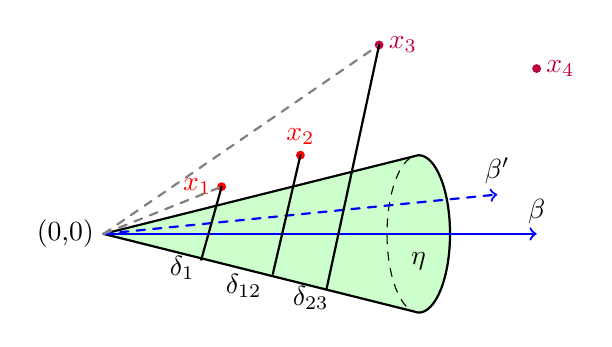
\begin{tikzpicture}[line cap=round,line join=round]

  % Funnel cone
  \path[fill=green!20,draw=black,thick]
    (0,0)                % apex
    -- (4,-1)            % bottom of ellipse
    arc [ start angle=-90, end angle=90,
           x radius=0.4, y radius=1, 
           xshift=4cm, yshift=0cm ]
    -- cycle;            % close back at apex
  
  % (Optional) show the full ellipse in dashed lines for reference
  \draw[dashed] (4,0) ellipse [x radius=0.4, y radius=1];
  
  % Label for the apex
  \node[left] at (0,0) {(0,0)};

  % Small arc for the angle s at the origin
    %\draw (0.5,0) arc[start angle=0, end angle=42, radius=0.6];
    \node at (4.,-0.35) {$\eta$};
  % Blue arrow labeled \beta
  \draw[->,blue,thick]
    (0,0)
    -- (5.5,0) 
    node[above,black] {$\bm{\beta}$};

    \draw[->,blue,dashed,thick]
    (0,0)
    -- (5,0.5) 
    node[above,black] {$\bm{\beta}'$};

    % Red rays x1 and x2
    \fill[red,thick] (1.5,0.6) circle (1.6pt) node[left]{$\bm{x}_1$};
    \fill[red,thick] (2.5,1.0) circle (1.6pt) node[above]{$\bm{x}_2$};
    
    % Purple points \bm{x}3 and x4 outside the cone
    \fill[purple] (3.5,2.4) circle (1.6pt) node[right]{$\bm{x}_3$};
    \fill[purple] (5.5,2.1) circle (1.6pt) node[right]{$\bm{x}_4$};

    \draw[dashed,gray,thick] (0,0) -- (1.5,0.6) node[left]{};
     \draw[dashed,gray,thick] (0,0) -- (3.5,2.4) node[left]{};

    \node at (1.0,-0.43) {$\delta_1$};
    \node at (1.78,-0.658) {$\delta_{12}$};
    \node at (2.63,-0.808) {$\delta_{23}$};
    %\node at (1.24,-0.33) node[left]{$\delta_{}$};
    \draw[thick,black,thick] (1.5,0.6) -- (1.24,-0.33) node[left]{};
    \draw[thick,black,thick] (2.5,1.0) -- (2.15,-0.508) node[left]{};
    \draw[thick,black,thick] (3.5,2.4) -- (2.83,-0.708) node[left]{};

\end{tikzpicture}

    \caption{Illustration of an $(\bm{\beta}, \delta,\eta)$-separated set and a sequence $(\bm{x}_1,\bm{x}_2,\bm{x}_3,\bm{x}_4)$ that satisfy the requirements of the definition. The distances $\delta_1, \delta_{12}, \delta_{23}$ are at least $\delta$ apart.\vspace{-3mm}}
    \label{fig: separated}
\end{figure}

In this section, we show a construction of a family of kernel machines $\curlybracket{f_n \in \cH(\reals^d)}$ such that the corresponding $\cR$-norm, i.e. $\curlybracket{\rtv{f_n}}$, diverges. 

%Assume that $\cX = \reals^d$. Let $\cN(\textbf{0}, 1)$ be a Gaussian distribution over $\cX$. 
% Define the Gaussian RKHS corresponding to a sequence of Mahalanbis matrices $\curlybracket{M_i \succ 0 : M_i \in \sf{Sym}_{+}(\reals^{d \times d})}$ as follows:
% \begin{align*}
%     \cH_n := \curlybracket{f: \cX \to \reals\,\bigg\lvert\, f(\cdot) = \sum_{i = i}^m \alpha_i \cdot K_{M_n}(x_i,\cdot),\, x_i \in \cX_n}
% \end{align*}
First, we state some useful assumptions on probabilist's Hermite polynomial which are easy to verify to hold in general (but surely in odd dimension $d$).

First assumption asserts that Gaussian weighted Hermite polynomial $H_{d+1}(y)e^{-\frac{y^2}{2}}$ has a peak within a finite interval around the origin.
% \begin{assumption}[$\delta$-peak]\label{ass: peak} Fix a dimension $d$. For a given Hermite polynomial $H_{d+1}$ we define an interval $\bracket{-\delta,\delta}$ as a region of $\delta$-peak if the following properties hold:
% \begin{enumerate}
%     \item for every $y > \delta$, $\frac{\partial H_{d+1}(y)e^{-\frac{y^2}{2}}}{\partial y} < 0$,
%     \item for every $y < \delta$, $\frac{\partial H_{d+1}(y)e^{-\frac{y^2}{2}}}{\partial y} > 0$.
% \end{enumerate}
% %a region of $\delta$-peak if     
% \end{assumption}
\begin{assumption}[$\delta$-peak]\label{ass: peak}
Fix a dimension $d$. For a given Hermite polynomial $H_{d+1}$, we call an interval $[-\delta,\delta]$ a region of $\delta$-peak if:
\begin{enumerate}
    \item $\frac{\partial H_{d+1}(y)e^{-\frac{y^2}{2}}}{\partial y} < 0$ for all $y > \delta$
    \item $\frac{\partial H_{d+1}(y)e^{-\frac{y^2}{2}}}{\partial y} > 0$ for all $y < -\delta$
\end{enumerate}
\end{assumption}
Due to exponential decay of the product $H_{d+1}(y)e^{-\frac{y^2}{2}}$, for any odd dimension $d$ note that 
$$\frac{\partial H_{d+1}(y)e^{-\frac{y^2}{2}}}{\partial y} = (H'_{d+1}(y) - yH_{d+1}(y))e^{-y^2/2}$$
where $-yH_{d+1}(y)$ is a polynomial with odd dimension with negative highest term and this implies there exists a $\delta$-peak.

Now, we state a trivial observation on the absolute integral of $H_{d+1}\left( y \right) \, e^{ -\frac{y^2}{2} }$. 
\begin{assumption}[$\epsilon$-safe]\label{ass: safe}
    We say a constant $\epsilon > 0$ is $\epsilon$-safe if $$\int_{[-\epsilon,\epsilon]} \left| H_{d+1}\left( y \right) \, e^{ -\frac{y^2}{2} }\right| \, dy > 0.$$
\end{assumption}
Since $H_{d+1}$ is non-zero polynomial this holds trivially for any $\epsilon > 0$. Furthermore, the integral is increasing with the size of an $\epsilon$-interval. 

With this, we state a useful result on the convergence of a series of evaluations of $H_{d+1}\left( y \right) \, e^{ -\frac{y^2}{2}}$ on distinct points $y \in \reals$. The proof is deferred to \iftoggle{longversion}{\appref{app: useful}}{the supplemental materials}.
% \begin{lemma}\label{lem: safeshift} result that states that for a sufficiently shifted centers/centers there is neighhood using Planchearel-Rotach theorem to show values for each Hermite polynomial is bounded
% \end{lemma}

% \begin{proof}
%     $$H_{d+1}(x) = (d+1)! \sum_{i=0}^{\lfloor (d+1)/2 \rfloor} \frac{(-1)^i x^{d+1-2i}}{(d+1-2i)!i! 2^i}$$
%     Now, we want an interval $[-\epsilon,\epsilon]$ such that
%     \begin{align*}
%         \int_{[-\epsilon,\epsilon]} \left| H_{d+1}\left( y \right) \, e^{ -\frac{y^2}{2} }\right| \, dy > 1
%     \end{align*}
%     Note that,
%     \begin{align*}
%         \int_{[-\epsilon,\epsilon]} \left| H_{d+1}\left( y \right) \, e^{ -\frac{y^2}{2} }\right| \, dy \ge 2\epsilon \cdot (d+1)! \sum_{i=0}^{\lfloor (d+1)/2 \rfloor} \frac{(-1)^i x^{d+1-2i}}{(d+1-2i)!i! 2^i} e^{-\frac{\epsilon^2}{2}}
%     \end{align*}

%     $$H_{d+1}(0) = (-1)^k(2k-1)!!$$
% \end{proof}

\begin{lemma}\label{lem: inter}
Let \( d\ge 0 \) be fixed and let \( H_{d+1}(y) \) denote the Hermite polynomial of degree \( d+1 \). Then for any constant $\rho > 0$, there exists a constant \( \delta_0 > 0 \) (depending only on \( d \)) such that for every \(\delta \ge \delta_0\) we have
\[
\sum_{j=2}^\infty \Bigl| H_{d+1}\bigl(j\delta\bigr) \Bigr|\, e^{-\frac{(j\delta)^2}{2}} < \frac{\rho}{4}.
\]
\end{lemma}


\subsection{Construction of a diverging sequence}

In \secref{sec: setup}, we defined the notions of $(\bm{\beta}, \delta, \eta)$-separated sets of size $n \in \mathbb{N}$. Let $(\bm{x}_1,\bm{x}_2,\ldots,\bm{x}_n)$ be a sequence in this set. Intuitively, any two centers in the sequence are at least $\delta$ apart when projected onto any direction $\bm{\beta}'$ such that $\bm{\beta}^{\mathsf{T}}\bm{\beta}' \ge \norm{\bm{\beta}}\norm{\bm{\beta}'}\eta$ (see \figref{fig: separated} for an illustration). Now, note that in \lemref{lem: cov}, we provided an alternate representation of the $\rtv{f}$ of a function as shown in \thmref{thm: rtv}, specifically the inner integral for each $\bm{\beta} \in \mathbb{S}^{d-1}$ has the form:
$$I_{\sf{inner}}(\bm{\beta}) := \int_{\mathbb{R}} \left| \sum_{i=1}^k \alpha_i H_{d+1}\left( y + \Delta_i \right) e^{ -\frac{(y + \Delta_i)^2}{2} } \right| dy$$
where each $\Delta_i = \bm{x}_1^\mathsf{T}\bm{\beta} - \bm{x}_i^\mathsf{T}\bm{\beta}$ (ignoring the normalization). If the projections $\bm{x}_i^\mathsf{T}\bm{\beta}$ are far apart on the real line $\reals$, noting the absolute decay in the values of $H_{d+1}\left( y \right) \, e^{ -\frac{y^2}{2} }$ outside the region of $\delta$-peak as asserted by \assref{ass: peak}, we can quantify and control contributions of terms corresponding to $j \neq i$ in the inner integral. 

Now, the property holds over a non-trivial cone $\cK(\bm{\beta}) := \curlybracket{\bm{\beta}' \in \mathbb{S}^{d-1}\,|\, \bm{\beta}^{\mathsf{T}}\bm{\beta}' \ge \eta }$ with non-zero volume. Now, noting the \eqnref{eq:transformed_I} which involves the second integral over the unit sphere $\mathbb{S}^{d-1}$, i.e.
$$\int_{\mathbb{S}^{d-1}} \frac{I_{\sf{inner}}(\bm{\beta})}{\sigma^{d+1}} \, d\bm{\beta}$$
is non-trivially positive. Thus, we crucially show along any direction $\bm{\beta}$ in the cone, $I_{\sf{inner}}$ diverges as $k$ grows if the kernel machine $f$ is defined for a sequence of centers from the $(\bm{\beta}, \delta, \eta)$-separated set.

 Now, we state the main theorem of the work. For ease of analysis we assume that the largest eigenvalue of $\mathbf{L}^{-1}$ is upper bounded by 1 which can be easily replaced with appropriate rescaling and choice of the parameters in the statement. 
% \akash{there should be a statement on why separated sets are convex! \exmref{exam: set} can be easily extended for the entire cone!}
 
\begin{theorem}[Diverging $\mathcal{R}\mathrm{TV}^2$]\label{thm: unbounded}
    Consider the Gaussian RKHS $\cH(\reals^d)$ as defined in \eqnref{eq: infinitegauss}. Assume $\epsilon \in (0,1/2]$ be a safe constant (see \assref{ass: safe}). Define \vspace{-2mm}
    \begin{align*}
        \rho :=  \int_{[-\epsilon,\epsilon]} \left| H_{d+1}\left( y \right) \, e^{ -\frac{y^2}{2} }\right| \, dy.\vspace{-2mm}
    \end{align*}
    Fix a unit vector $\bm{\beta} \in \reals^d$, scalars $\eta \ge \frac{\sqrt{3}}{2}$, and $\delta = 3\max\{\epsilon, \delta_0(\rho), \delta'\}$ where $\delta_0(\rho)$ is chosen as per \lemref{lem: inter}, and $\delta'(d)$ as per \assref{ass: peak}. Let $\cX_\infty = \curlybracket{\bm{x}_1,\bm{x}_2,\ldots} \subset \reals^d$ be an infinite sequence such that any subsequence $\Gamma_n = \curlybracket{\bm{x}_1,\bm{x}_2,\ldots, \bm{x}_n}$ is in the $(\bm{\beta}, \delta, \eta)$-separated set of size $n$. Define a function $f \in \cH$ on $\cX_\infty$ that has a representation with an $f$-unbounded combination $\alpha_f$. Then,% and centers $\{x^{(n)}_1,\ldots,x^{(n)}_n\} \in \Gamma_n$. Then, if $s$
    % Let $f_n \in \cH$ be a classifer with combination $\alpha_n$ and centers $\{x^{(n)}_1,\ldots,x^{(n)}_n\} \in \Gamma_n$. Then, if $$
    %$\Gamma_n \subset \cH$ is a $(\beta, \delta, \eta)$-separated set of size $n$.
    \begin{align}
        \rtv{\{f_n\}} \to \infty
    \end{align}
\end{theorem}

\begin{proof}
    %\akash{you start with fixing some $\epsilon >0$ for which you get some $\rho$, which you use to pick one bound on $\delta$. Either adjust $\eta$ for $\delta$ or vice versa.  I mean if $\eta$ is large then $\delta$ needs to be large as well}
    First, we rewrite \eqnref{eq:transformed_I} for the $\cR$-norm of the function $f_k$ as follows
    \begin{align*}
        \rtv{f_k} &= \frac{1}{|\det \mathbf{L}| \sqrt{2\pi}} \int_{\mathbb{S}^{d-1}} \frac{1}{\sigma^{d+1}} \int_{\mathbb{R}} \left| \sum_{i=1}^k \alpha_i H_{d+1}\left( y + \Delta_i \right) e^{ -\frac{(y + \Delta_i)^2}{2} } \right| dy \, d\bm{\beta} 
    \end{align*}
    with the inner integral \vspace{-2mm}
    \[I_{\sf{inner}}(\bm{\beta}) = \int_{\reals} \left| \sum_{i=1}^k \alpha_i \, H_{d+1}\left( y + \Delta_i \right) \, e^{ -\frac{(y + \Delta_i)^2}{2} } \right| \, dy
\]
where:
\[
\Delta_1 = 0,\,\,\Delta_i = \frac{a_1 - a_i}{\sigma} = \frac{\bm{x}_1^\mathsf{T}\bm{\beta} - \bm{x}_i^\mathsf{T}\bm{\beta}}{\|\mathbf{L}^{-\mathsf{T}}\bm{\beta}\|}
\quad \text{for } i = 2, 3, \ldots, k.
\]
First, define the cone $\cK$ wrt $\bm{\beta}$ and $\eta$ as stated in the theorem statement, i.e.
\begin{align*}
    \cK := \curlybracket{\bm{\beta}' \in \mathbb{S}^{d-1}\,|\, \bm{\beta}'^{\mathsf{T}} \bm{\beta} \ge \eta}
\end{align*}
Note that the volume $\vol{\cK} > 0$ implying that 
\begin{align}
    \int_{\mathbb{S}^{d-1}} \frac{1}{\sigma^{d+1}} \, d\bm{\bm{\beta}} \ge  \int_{\cK} \frac{1}{\sigma^{d+1}} \, d\bm{\beta} = (\star) \label{eq: cone}
\end{align}
    Note that $\mathbf{M} = \mathbf{L}^\mathsf{T}\mathbf{L}$. We assume that the $\mathbf{M}$ is symmetric and PSD, implying that singular values of $\mathbf{L}$ are \tt{exactly} the square root of the eigenvalues of $\mathbf{M}$, i.e
    \[ \sigma_i(\mathbf{L}) = \sqrt{|\lambda_i(\mathbf{M})|}\]
    \looseness-1 But since $\mathbf{L}$ is invertible implying the singular values if $\mathbf{L^{-1}}$ are inverses to singular values of $\mathbf{L}$, i.e. $\sigma_i(\mathbf{L}^{-1}) = \frac{1}{\sigma_i(\mathbf{L})}$.
    Thus, we can rewrite \eqnref{eq: cone} as
    \begin{align}
     (\star) =  \int_{\cK} \frac{1}{\sigma_{\max}(\mathbf{L}^{-1})^{d+1}} \, d\bm{\beta} \ge \int_{\cK} \sigma_{\min}(\mathbf{L})^{d+1} \, d\bm{\beta} = \int_{\cK} \lambda_{\min}(\mathbf{M})^{\frac{(d+1)}{2}} \, d\bm{\beta} =  \lambda_{\min}(\mathbf{M})^{\frac{(d+1)}{2}} \vol{\cK} > 0 \label{eq: vol}
    \end{align}
    Now, we will show for any $\bm{\beta}' \in \cK$, there is a non-trivial lower bound on $I_{\sf{inner}}(\bm{\beta}')$. Note that by definition, $\Gamma_n$ is in the $(\bm{\beta}',\delta)$-separated set. 

    Hence, for all $i,j = 2, 3, \ldots$
    \begin{align*}
        |\Delta_i - \Delta_j| \ge \delta
    \end{align*}
    Define the neighborhoods $\curlybracket{N_i}$ for the safe constant $\epsilon$ as follows
    $$N_i := \bracket{-\Delta_i - \epsilon, -\Delta_i + \epsilon}.$$
    %But using \lemref{lem: safeshift}, we know that there exists $\epsilon > 0$ and 
    Now, consider the integral on the neighborhood $N_i$:
    \begin{align*}
        &\int_{N_i} \left| \sum_{i=1}^k \alpha_i \, H_{d+1}\left( y + \Delta_i \right) \, e^{ -\frac{(y + \Delta_i)^2}{2} } \right| \, dy \\
        &\ge \int_{N_i} \left|\alpha_i \, H_{d+1}\left( y + \Delta_i \right) \, e^{ -\frac{(y + \Delta_i)^2}{2} } \right| \, dy - \underbrace{\int_{N_i} \left| \sum_{j=1, j \neq i}^k \alpha_j \, H_{d+1}\left( y + \Delta_j \right) \, e^{ -\frac{(y + \Delta_j)^2}{2} } \right| \, dy}_{=: \large{\theta_i}}\\ 
        &\hspace{100mm}\text{(triangle inequality)}\\
        &\ge |\alpha_i| \int_{[-\epsilon,\epsilon]} \left|H_{d+1}\left( y \right) \, e^{ -\frac{y^2}{2} } \right| \, dy - \theta_i \hspace{38.5mm}\text{(change of variable)} \\ 
        &\ge |\alpha_i| \rho - \theta_i \hspace{85mm}\text{(definition of $\rho$)}
    \end{align*}

    Summing over each $i = 1, 2, \ldots k$, we get
    \begin{align}
        I_{\sf{inner}} &\ge \sum_{i = 1}^k \int_{N_i} \left| \sum_{i=1}^k \alpha_i \, H_{d+1}\left( y + \Delta_i \right) \, e^{ -\frac{(y + \Delta_i)^2}{2} } \right| \, dy \nonumber\\
        & \ge \rho \sum_{i=1}^k |\alpha_i| - \sum_{i=1}^k \theta_i \label{eq: diff}
    \end{align}
     %\akash{show why the negative term is bounded}
    Now, we will show how to bound the sum $\sum_{i=1}^k \theta_i$.%\akash{show why $|i-j|\delta$ diff work below}
    \paragraph{Bounding $\theta_k$:} First note that, we can bound each $\theta_i$ as follows\vspace{-5mm}
    \allowdisplaybreaks
    \begin{center}
    \begin{align*}
        \theta_i &= \int_{N_i} \left| \sum_{j=1, j \neq i}^k \alpha_j \, H_{d+1}\left( y + \Delta_j \right) \, e^{ -\frac{(y + \Delta_j)^2}{2} } \right| \, dy \\ &\le  \sum_{j=1, j \neq i}^k \int_{N_i} \left|  \alpha_j \, H_{d+1}\left( y + \Delta_j \right) \, e^{ -\frac{(y + \Delta_j)^2}{2} } \right| \, dy \quad &\text{(triangle inequality)}\\
        &\le  \sum_{j=1, j \neq i}^k \int_{\bracket{-\epsilon,\epsilon}} \left|  \alpha_j \, H_{d+1}\left(-\Delta_i + y + \Delta_j \right) \, e^{ -\frac{(-\Delta_i + y + \Delta_j)^2}{2} } \right| \, dy &\text{(change of variable)}\\
        & \le \sum_{j=1, j \neq i}^k |\alpha_j| \int_{\bracket{-\epsilon,\epsilon}}  \left| H_{d+1}\left( |i-j|\delta \right) \, e^{ -\frac{(|i-j| \delta)^2}{2} } \right| \, dy \quad &\text{($\delta$-peak)} \\
        %& \le \sum_{j=1, j \neq i}^k |\alpha_j| \int_{N_i}  \left| H_{d+1}\left( j\delta \right) \, e^{ -\frac{(j \delta)^2}{2} } \right| \, dy \\
        & \le 2 \epsilon \sum_{j=1, j \neq i}^k |\alpha_j| \left|H_{d+1}\left( |i-j|\delta \right)\right| \, e^{ -\frac{(|i-j| \delta)^2}{2} } \\
        & \le \sum_{j=1, j \neq i}^k |\alpha_j| \left|H_{d+1}\left( |i-j|\delta \right)\right| \, e^{ -\frac{(|i-j| \delta)^2}{2} } \quad &\text{($\epsilon \le 1/2$)}
        %&\le (k-1) H_{d+1}\left( 2\delta \right) \, e^{ -\frac{(2 \delta)^2}{2} } \sum_{j=1}^k |\alpha_j| \\
        %& \le C_{2\delta} (k-1) \sum_{i=1}^k |\alpha_i|
    \end{align*}
    \end{center}
    To simplify $-\Delta_i + y + \Delta_j$ for a choice of $y \in \bracket{-\epsilon,\epsilon}$, we assume that indices of the projections $\Delta_i$ for $i = 1,2, \ldots$ are arranged in ascending order in their values on the real line. Since each consecutive projections are at least $\delta$ apart, we can bound $|-\Delta_i + y + \Delta_j| > (|i-j| - 1/3)\delta$. Since Hermite polynomials in even dimension, i.e. $d+1$, are even 
    \begin{align*}
      \left|H_{d+1}\left(-\Delta_i + y + \Delta_j \right) \, e^{ -\frac{(-\Delta_i + y + \Delta_j)^2}{2}}\right| \le \left| H_{d+1}\left((|i - j| - 2/3)\delta\right) e^{ -\frac{((|i - j| - 2/3)\delta)^2}{2}} \right|  
    \end{align*}
    For simplification, we have omitted the $-(2/3)\delta$ additive term in the equation above.

    Summing over each $i = 1,\ldots,k$
    \begin{align*}
        \sum_{i=1}^k \theta_k &= \sum_{i=1}^k \int_{N_i} \left| \sum_{j=1, j \neq i}^k \alpha_j \, H_{d+1}\left( y + \Delta_j \right) \, e^{ -\frac{(y + \Delta_j)^2}{2} } \right| \, dy \\
        &\le \sum_{i=1}^k \sum_{j=1, j \neq i}^k |\alpha_j| \left|H_{d+1}\left( |i-j|\delta \right)\right| \, e^{ -\frac{(|i-j| \delta)^2}{2} }\\
        &\le 2\paren{\sum_{j=1}^{k}  \left|H_{d+1}\left( j\delta \right) \right|\, e^{ -\frac{(j \delta)^2}{2} }} \sum_{i=1}^k |\alpha_i|
    \end{align*}
    Using \lemref{lem: inter}, we can rewrite \eqnref{eq: diff}
    \begin{align}
        I_{\sf{inner}} \ge \rho \sum_{i=1}^k |\alpha_i| - 2\paren{\sum_{j=2}^k  \left|H_{d+1}\left( j\delta \right)\right| \, e^{ -\frac{(j \delta)^2}{2} }} \sum_{i=1}^k |\alpha_i| \ge \frac{\rho}{2}\sum_{i=1}^k |\alpha_i| 
    \end{align}
    % Now, in the limiting case
    % \begin{align*}
    %     \lim_{k \to \infty}  I_{\sf{inner}}(\bm{\beta}') \ge \lim_{k \to \infty} \rho \sum_{i=1}^k |\alpha_i| - \lim_{k \to \infty} \sum_{i=1}^k \theta_k \ge \frac{\rho}{2} \norm{\alpha_f}_{\ell_1}
    % \end{align*}
    % Since $\rho > 0$, we have $\frac{\rho}{2} \norm{\alpha_f}_{\ell_1} \to \infty$ as $ \norm{\alpha_f}_{\ell_1}$ is unbounded.

    % Since $\bm{\beta}'$ was arbitrarily picked from the cone $\cK$, for all $\bm{\beta}' \in \cK$
    % \begin{align}
    %      \lim_{k \to \infty}  I_{\sf{inner}}(\bm{\beta}') \to \infty \label{eq: limit}
    % \end{align}
    \noindent Now, note that using \eqnref{eq: cone} and \eqnref{eq: vol}
    \begin{align*}
        \rtv{f_k} &\ge \frac{1}{|\det \mathbf{L}| \sqrt{2\pi}} \int_{\cK} \frac{1}{\sigma^{d+1}} \int_{\mathbb{R}} \left| \sum_{i=1}^k \alpha_i H_{d+1}\left( y + \Delta_i \right) e^{ -\frac{(y + \Delta_i)^2}{2} } \right| dy \, d\bm{\beta} \\
        & \ge \frac{1}{|\det \mathbf{L}| \sqrt{2\pi}} \int_{\cK} \frac{1}{\sigma^{d+1}}  \paren{\frac{\rho}{2}\sum_{i=1}^k |\alpha_i| } \, d\bm{\beta}\\
        & \ge \paren{\frac{1}{|\det \mathbf{L}| \sqrt{2\pi}} \lambda_{\min}(\mathbf{M})^{\frac{(d+1)} {2}} \vol{\cK}} \cdot\paren{\frac{\rho}{2}\sum_{i=1}^k |\alpha_i| }
    \end{align*}
    Now, in the limiting case
    \begin{align*}
        \lim_{k \to \infty} \rtv{f_k} &\ge \paren{\frac{1}{|\det \mathbf{L}| \sqrt{2\pi}} \lambda_{\min}(\mathbf{M})^{\frac{(d+1)} {2}} \vol{\cK}} \lim_{k \to \infty} \paren{\frac{\rho}{2}\sum_{i=1}^k |\alpha_i| } \\
        & =  \paren{\frac{1}{|\det \mathbf{L}| \sqrt{2\pi}} \lambda_{\min}(\mathbf{M})^{\frac{(d+1)} {2}} \vol{\cK}} \cdot \frac{\rho}{2} \norm{\alpha_f} \to \infty
    \end{align*}
    Hence the claim of the theorem has been proven.
\end{proof}
%\akash{ should fix $\rho > 1$, it depends on choice of $\epsilon$ which will affect $\delta$ as well}
    
    
    
    
    % Now, consider the following bound
    % \begin{align*}
    %     \frac{1}{\norm{\mathbf{L}^{-\mathsf{T}}\bm{\beta}}} \le \frac{1}{\sigma_{\min}(\mathbf{L}^{-1})} = \sigma_{\max}(\mathbf{L}) = \sqrt{\lambda_{\max}(\mathbf{M})}
    % \end{align*}
    % Thus, we can write 
    % \[
    % \cA \le \lambda_{\max}(\mathbf{M})^{\frac{d+1}{2}} \cdot \int_{\mathbb{S}^{d-1}} \,\mathrm{d}\bm{\beta} = \lambda_{\max}(\mathbf{M})^{\frac{d+1}{2}} \cdot\frac{2\pi^{\frac{d}{2}}}{\Gamma\paren{\frac{d}{2}}}
    % \]
    % where $\Gamma$ is a \textbf{Gamma} function.
    % Since $\lambda_{\max}(\mathbf{M})$ is a bounded value, we note that $\cA$ is bounded above by a constant that depends on the largest eigenvalue of $\mathbf{M}$ and the dimension $d$.
    % \end{proof}
% \end{proof}


%
\begin{table*}[t]
\centering
\fontsize{11pt}{11pt}\selectfont
\begin{tabular}{lllllllllllll}
\toprule
\multicolumn{1}{c}{\textbf{task}} & \multicolumn{2}{c}{\textbf{Mir}} & \multicolumn{2}{c}{\textbf{Lai}} & \multicolumn{2}{c}{\textbf{Ziegen.}} & \multicolumn{2}{c}{\textbf{Cao}} & \multicolumn{2}{c}{\textbf{Alva-Man.}} & \multicolumn{1}{c}{\textbf{avg.}} & \textbf{\begin{tabular}[c]{@{}l@{}}avg.\\ rank\end{tabular}} \\
\multicolumn{1}{c}{\textbf{metrics}} & \multicolumn{1}{c}{\textbf{cor.}} & \multicolumn{1}{c}{\textbf{p-v.}} & \multicolumn{1}{c}{\textbf{cor.}} & \multicolumn{1}{c}{\textbf{p-v.}} & \multicolumn{1}{c}{\textbf{cor.}} & \multicolumn{1}{c}{\textbf{p-v.}} & \multicolumn{1}{c}{\textbf{cor.}} & \multicolumn{1}{c}{\textbf{p-v.}} & \multicolumn{1}{c}{\textbf{cor.}} & \multicolumn{1}{c}{\textbf{p-v.}} &  &  \\ \midrule
\textbf{S-Bleu} & 0.50 & 0.0 & 0.47 & 0.0 & 0.59 & 0.0 & 0.58 & 0.0 & 0.68 & 0.0 & 0.57 & 5.8 \\
\textbf{R-Bleu} & -- & -- & 0.27 & 0.0 & 0.30 & 0.0 & -- & -- & -- & -- & - &  \\
\textbf{S-Meteor} & 0.49 & 0.0 & 0.48 & 0.0 & 0.61 & 0.0 & 0.57 & 0.0 & 0.64 & 0.0 & 0.56 & 6.1 \\
\textbf{R-Meteor} & -- & -- & 0.34 & 0.0 & 0.26 & 0.0 & -- & -- & -- & -- & - &  \\
\textbf{S-Bertscore} & \textbf{0.53} & 0.0 & {\ul 0.80} & 0.0 & \textbf{0.70} & 0.0 & {\ul 0.66} & 0.0 & {\ul0.78} & 0.0 & \textbf{0.69} & \textbf{1.7} \\
\textbf{R-Bertscore} & -- & -- & 0.51 & 0.0 & 0.38 & 0.0 & -- & -- & -- & -- & - &  \\
\textbf{S-Bleurt} & {\ul 0.52} & 0.0 & {\ul 0.80} & 0.0 & 0.60 & 0.0 & \textbf{0.70} & 0.0 & \textbf{0.80} & 0.0 & {\ul 0.68} & {\ul 2.3} \\
\textbf{R-Bleurt} & -- & -- & 0.59 & 0.0 & -0.05 & 0.13 & -- & -- & -- & -- & - &  \\
\textbf{S-Cosine} & 0.51 & 0.0 & 0.69 & 0.0 & {\ul 0.62} & 0.0 & 0.61 & 0.0 & 0.65 & 0.0 & 0.62 & 4.4 \\
\textbf{R-Cosine} & -- & -- & 0.40 & 0.0 & 0.29 & 0.0 & -- & -- & -- & -- & - & \\ \midrule
\textbf{QuestEval} & 0.23 & 0.0 & 0.25 & 0.0 & 0.49 & 0.0 & 0.47 & 0.0 & 0.62 & 0.0 & 0.41 & 9.0 \\
\textbf{LLaMa3} & 0.36 & 0.0 & \textbf{0.84} & 0.0 & {\ul{0.62}} & 0.0 & 0.61 & 0.0 &  0.76 & 0.0 & 0.64 & 3.6 \\
\textbf{our (3b)} & 0.49 & 0.0 & 0.73 & 0.0 & 0.54 & 0.0 & 0.53 & 0.0 & 0.7 & 0.0 & 0.60 & 5.8 \\
\textbf{our (8b)} & 0.48 & 0.0 & 0.73 & 0.0 & 0.52 & 0.0 & 0.53 & 0.0 & 0.7 & 0.0 & 0.59 & 6.3 \\  \bottomrule
\end{tabular}
\caption{Pearson correlation on human evaluation on system output. `R-': reference-based. `S-': source-based.}
\label{tab:sys}
\end{table*}



\begin{table}%[]
\centering
\fontsize{11pt}{11pt}\selectfont
\begin{tabular}{llllll}
\toprule
\multicolumn{1}{c}{\textbf{task}} & \multicolumn{1}{c}{\textbf{Lai}} & \multicolumn{1}{c}{\textbf{Zei.}} & \multicolumn{1}{c}{\textbf{Scia.}} & \textbf{} & \textbf{} \\ 
\multicolumn{1}{c}{\textbf{metrics}} & \multicolumn{1}{c}{\textbf{cor.}} & \multicolumn{1}{c}{\textbf{cor.}} & \multicolumn{1}{c}{\textbf{cor.}} & \textbf{avg.} & \textbf{\begin{tabular}[c]{@{}l@{}}avg.\\ rank\end{tabular}} \\ \midrule
\textbf{S-Bleu} & 0.40 & 0.40 & 0.19* & 0.33 & 7.67 \\
\textbf{S-Meteor} & 0.41 & 0.42 & 0.16* & 0.33 & 7.33 \\
\textbf{S-BertS.} & {\ul0.58} & 0.47 & 0.31 & 0.45 & 3.67 \\
\textbf{S-Bleurt} & 0.45 & {\ul 0.54} & {\ul 0.37} & 0.45 & {\ul 3.33} \\
\textbf{S-Cosine} & 0.56 & 0.52 & 0.3 & {\ul 0.46} & {\ul 3.33} \\ \midrule
\textbf{QuestE.} & 0.27 & 0.35 & 0.06* & 0.23 & 9.00 \\
\textbf{LlaMA3} & \textbf{0.6} & \textbf{0.67} & \textbf{0.51} & \textbf{0.59} & \textbf{1.0} \\
\textbf{Our (3b)} & 0.51 & 0.49 & 0.23* & 0.39 & 4.83 \\
\textbf{Our (8b)} & 0.52 & 0.49 & 0.22* & 0.43 & 4.83 \\ \bottomrule
\end{tabular}
\caption{Pearson correlation on human ratings on reference output. *not significant; we cannot reject the null hypothesis of zero correlation}
\label{tab:ref}
\end{table}


\begin{table*}%[]
\centering
\fontsize{11pt}{11pt}\selectfont
\begin{tabular}{lllllllll}
\toprule
\textbf{task} & \multicolumn{1}{c}{\textbf{ALL}} & \multicolumn{1}{c}{\textbf{sentiment}} & \multicolumn{1}{c}{\textbf{detoxify}} & \multicolumn{1}{c}{\textbf{catchy}} & \multicolumn{1}{c}{\textbf{polite}} & \multicolumn{1}{c}{\textbf{persuasive}} & \multicolumn{1}{c}{\textbf{formal}} & \textbf{\begin{tabular}[c]{@{}l@{}}avg. \\ rank\end{tabular}} \\
\textbf{metrics} & \multicolumn{1}{c}{\textbf{cor.}} & \multicolumn{1}{c}{\textbf{cor.}} & \multicolumn{1}{c}{\textbf{cor.}} & \multicolumn{1}{c}{\textbf{cor.}} & \multicolumn{1}{c}{\textbf{cor.}} & \multicolumn{1}{c}{\textbf{cor.}} & \multicolumn{1}{c}{\textbf{cor.}} &  \\ \midrule
\textbf{S-Bleu} & -0.17 & -0.82 & -0.45 & -0.12* & -0.1* & -0.05 & -0.21 & 8.42 \\
\textbf{R-Bleu} & - & -0.5 & -0.45 &  &  &  &  &  \\
\textbf{S-Meteor} & -0.07* & -0.55 & -0.4 & -0.01* & 0.1* & -0.16 & -0.04* & 7.67 \\
\textbf{R-Meteor} & - & -0.17* & -0.39 & - & - & - & - & - \\
\textbf{S-BertScore} & 0.11 & -0.38 & -0.07* & -0.17* & 0.28 & 0.12 & 0.25 & 6.0 \\
\textbf{R-BertScore} & - & -0.02* & -0.21* & - & - & - & - & - \\
\textbf{S-Bleurt} & 0.29 & 0.05* & 0.45 & 0.06* & 0.29 & 0.23 & 0.46 & 4.2 \\
\textbf{R-Bleurt} & - &  0.21 & 0.38 & - & - & - & - & - \\
\textbf{S-Cosine} & 0.01* & -0.5 & -0.13* & -0.19* & 0.05* & -0.05* & 0.15* & 7.42 \\
\textbf{R-Cosine} & - & -0.11* & -0.16* & - & - & - & - & - \\ \midrule
\textbf{QuestEval} & 0.21 & {\ul{0.29}} & 0.23 & 0.37 & 0.19* & 0.35 & 0.14* & 4.67 \\
\textbf{LlaMA3} & \textbf{0.82} & \textbf{0.80} & \textbf{0.72} & \textbf{0.84} & \textbf{0.84} & \textbf{0.90} & \textbf{0.88} & \textbf{1.00} \\
\textbf{Our (3b)} & 0.47 & -0.11* & 0.37 & 0.61 & 0.53 & 0.54 & 0.66 & 3.5 \\
\textbf{Our (8b)} & {\ul{0.57}} & 0.09* & {\ul 0.49} & {\ul 0.72} & {\ul 0.64} & {\ul 0.62} & {\ul 0.67} & {\ul 2.17} \\ \bottomrule
\end{tabular}
\caption{Pearson correlation on human ratings on our constructed test set. 'R-': reference-based. 'S-': source-based. *not significant; we cannot reject the null hypothesis of zero correlation}
\label{tab:con}
\end{table*}

\section{Results}
We benchmark the different metrics on the different datasets using correlation to human judgement. For content preservation, we show results split on data with system output, reference output and our constructed test set: we show that the data source for evaluation leads to different conclusions on the metrics. In addition, we examine whether the metrics can rank style transfer systems similar to humans. On style strength, we likewise show correlations between human judgment and zero-shot evaluation approaches. When applicable, we summarize results by reporting the average correlation. And the average ranking of the metric per dataset (by ranking which metric obtains the highest correlation to human judgement per dataset). 

\subsection{Content preservation}
\paragraph{How do data sources affect the conclusion on best metric?}
The conclusions about the metrics' performance change radically depending on whether we use system output data, reference output, or our constructed test set. Ideally, a good metric correlates highly with humans on any data source. Ideally, for meta-evaluation, a metric should correlate consistently across all data sources, but the following shows that the correlations indicate different things, and the conclusion on the best metric should be drawn carefully.

Looking at the metrics correlations with humans on the data source with system output (Table~\ref{tab:sys}), we see a relatively high correlation for many of the metrics on many tasks. The overall best metrics are S-BertScore and S-BLEURT (avg+avg rank). We see no notable difference in our method of using the 3B or 8B model as the backbone.

Examining the average correlations based on data with reference output (Table~\ref{tab:ref}), now the zero-shoot prompting with LlaMA3 70B is the best-performing approach ($0.59$ avg). Tied for second place are source-based cosine embedding ($0.46$ avg), BLEURT ($0.45$ avg) and BertScore ($0.45$ avg). Our method follows on a 5. place: here, the 8b version (($0.43$ avg)) shows a bit stronger results than 3b ($0.39$ avg). The fact that the conclusions change, whether looking at reference or system output, confirms the observations made by \citet{scialom-etal-2021-questeval} on simplicity transfer.   

Now consider the results on our test set (Table~\ref{tab:con}): Several metrics show low or no correlation; we even see a significantly negative correlation for some metrics on ALL (BLEU) and for specific subparts of our test set for BLEU, Meteor, BertScore, Cosine. On the other end, LlaMA3 70B is again performing best, showing strong results ($0.82$ in ALL). The runner-up is now our 8B method, with a gap to the 3B version ($0.57$ vs $0.47$ in ALL). Note our method still shows zero correlation for the sentiment task. After, ranks BLEURT ($0.29$), QuestEval ($0.21$), BertScore ($0.11$), Cosine ($0.01$).  

On our test set, we find that some metrics that correlate relatively well on the other datasets, now exhibit low correlation. Hence, with our test set, we can now support the logical reasoning with data evidence: Evaluation of content preservation for style transfer needs to take the style shift into account. This conclusion could not be drawn using the existing data sources: We hypothesise that for the data with system-based output, successful output happens to be very similar to the source sentence and vice versa, and reference-based output might not contain server mistakes as they are gold references. Thus, none of the existing data sources tests the limits of the metrics.  


\paragraph{How do reference-based metrics compare to source-based ones?} Reference-based metrics show a lower correlation than the source-based counterpart for all metrics on both datasets with ratings on references (Table~\ref{tab:sys}). As discussed previously, reference-based metrics for style transfer have the drawback that many different good solutions on a rewrite might exist and not only one similar to a reference.


\paragraph{How well can the metrics rank the performance of style transfer methods?}
We compare the metrics' ability to judge the best style transfer methods w.r.t. the human annotations: Several of the data sources contain samples from different style transfer systems. In order to use metrics to assess the quality of the style transfer system, metrics should correctly find the best-performing system. Hence, we evaluate whether the metrics for content preservation provide the same system ranking as human evaluators. We take the mean of the score for every output on each system and the mean of the human annotations; we compare the systems using the Kendall's Tau correlation. 

We find only the evaluation using the dataset Mir, Lai, and Ziegen to result in significant correlations, probably because of sparsity in a number of system tests (App.~\ref{app:dataset}). Our method (8b) is the only metric providing a perfect ranking of the style transfer system on the Lai data, and Llama3 70B the only one on the Ziegen data. Results in App.~\ref{app:results}. 


\subsection{Style strength results}
%Evaluating style strengths is a challenging task. 
Llama3 70B shows better overall results than our method. However, our method scores higher than Llama3 70B on 2 out of 6 datasets, but it also exhibits zero correlation on one task (Table~\ref{tab:styleresults}).%More work i s needed on evaluating style strengths. 
 
\begin{table}%[]
\fontsize{11pt}{11pt}\selectfont
\begin{tabular}{lccc}
\toprule
\multicolumn{1}{c}{\textbf{}} & \textbf{LlaMA3} & \textbf{Our (3b)} & \textbf{Our (8b)} \\ \midrule
\textbf{Mir} & 0.46 & 0.54 & \textbf{0.57} \\
\textbf{Lai} & \textbf{0.57} & 0.18 & 0.19 \\
\textbf{Ziegen.} & 0.25 & 0.27 & \textbf{0.32} \\
\textbf{Alva-M.} & \textbf{0.59} & 0.03* & 0.02* \\
\textbf{Scialom} & \textbf{0.62} & 0.45 & 0.44 \\
\textbf{\begin{tabular}[c]{@{}l@{}}Our Test\end{tabular}} & \textbf{0.63} & 0.46 & 0.48 \\ \bottomrule
\end{tabular}
\caption{Style strength: Pearson correlation to human ratings. *not significant; we cannot reject the null hypothesis of zero corelation}
\label{tab:styleresults}
\end{table}

\subsection{Ablation}
We conduct several runs of the methods using LLMs with variations in instructions/prompts (App.~\ref{app:method}). We observe that the lower the correlation on a task, the higher the variation between the different runs. For our method, we only observe low variance between the runs.
None of the variations leads to different conclusions of the meta-evaluation. Results in App.~\ref{app:results}.
%\section{Infinite dimensional RKBS}

We will prove that the Banach space
\[
\mathcal{B} = \left\{ f : f(x) = \sum_{i=1}^\infty \alpha_i\,\lambda_i\, e_i(x),\quad \|f\|_{\mathcal{B}} = \left(\sum_{i=1}^\infty |\alpha_i\,\lambda_i|^p\right)^{1/p} < \infty \right\}
\]
has the following properties:
\begin{itemize}
    \item It is complete (i.e. it is a Banach space).
    \item Each evaluation functional \(\delta_x: f\mapsto f(x)\) is continuous.
    \item Its dual space is naturally given by
   \[
   \mathcal{B}^* \cong \left\{ g : g(x)=\sum_{i=1}^\infty \beta_i\, e_i'(x),\quad \|g\|_{\mathcal{B}^*} = \left(\sum_{i=1}^\infty \Bigl|\frac{\beta_i}{\lambda_i}\Bigr|^q\right)^{1/q} < \infty \right\},
   \]
   where \(1/p+1/q=1\) and the dual functionals \(e_i'\) satisfy \(e_i'(e_j)=\delta_{ij}\).
\end{itemize}
 

In what follows we will give full proofs of these facts.


\paragraph{Completeness of \(\mathcal{B}\)}

First, we show that $\cB$  has an isometric identification with \(\ell^p\)

Every \(f\in\mathcal{B}\) has a unique expansion
\[
f(x)= \sum_{i=1}^\infty \alpha_i\,\lambda_i\, e_i(x)
\]
with norm
\[
\|f\|_{\mathcal{B}} = \left(\sum_{i=1}^\infty |\alpha_i\,\lambda_i|^p\right)^{1/p}.
\]
Define the linear mapping
\[
T:\mathcal{B}\to \ell^p,\quad T(f)=(\alpha_i\,\lambda_i)_{i\ge1}.
\]
Then
\[
\|T(f)\|_{\ell^p} = \left(\sum_{i=1}^\infty |\alpha_i\,\lambda_i|^p\right)^{1/p} = \|f\|_{\mathcal{B}},
\]
so \(T\) is an isometry (i.e. it preserves the norm).

Since \(\ell^p\) is a well-known Banach space (i.e. it is complete), the image \(T(\mathcal{B})\) is a closed subspace of \(\ell^p\) (or, at least, one may complete the space and then identify it with a closed subspace). Therefore, every Cauchy sequence \(\{f_n\}\) in \(\mathcal{B}\) is such that \(\{T(f_n)\}\) is a Cauchy sequence in \(\ell^p\) and hence converges in \(\ell^p\) to some limit \(c=(c_i)_{i\ge1}\). Defining \(\alpha_i\) by \(c_i=\alpha_i\,\lambda_i\) (with the obvious convention when \(\lambda_i=0\)), we see that there exists an \(f\in\mathcal{B}\) with \(T(f)=c\). Thus, \(f_n\to f\) in \(\mathcal{B}\). In other words, \(\mathcal{B}\) is complete.

---

\paragraph{Continuity of the Evaluation Functional}

Let \(x\) be an arbitrary point in the domain. We want to show that the evaluation functional
\[
\delta_x : \mathcal{B} \to \mathbb{K},\quad \delta_x(f)=f(x)
\]
is continuous. (Here, \(\mathbb{K}\) denotes \(\mathbb{R}\) or \(\mathbb{C}\).)

Step 2.1. Direct Estimate Using Hölder’s Inequality

Given \(f\in\mathcal{B}\) with
\[
f(x)=\sum_{i=1}^\infty \alpha_i\,\lambda_i\, e_i(x),
\]
by Hölder’s inequality we have
\[
|f(x)| \le \sum_{i=1}^\infty |\alpha_i\,\lambda_i|\, |e_i(x)|
\le \left(\sum_{i=1}^\infty |\alpha_i\,\lambda_i|^p\right)^{1/p}\left(\sum_{i=1}^\infty |e_i(x)|^q\right)^{1/q}.
\]
That is,
\[
|f(x)| \le \|f\|_{\mathcal{B}}\,\left(\sum_{i=1}^\infty |e_i(x)|^q\right)^{1/q}.
\]
Thus, the evaluation functional satisfies
\[
|\delta_x(f)| \le C(x)\|f\|_{\mathcal{B}},\quad \text{with } C(x)=\left(\sum_{i=1}^\infty |e_i(x)|^q\right)^{1/q}.
\]
In order for this estimate to be useful, we assume that for every \(x\) the series
\[
\sum_{i=1}^\infty |e_i(x)|^q
\]
converges. (This is a common assumption when one constructs a reproducing kernel Banach space from a given basis.)

Step 2.2. Representer of Evaluation

An equivalent way to show that \(\delta_x\) is continuous is to exhibit a representer in the dual space \(\mathcal{B}^*\). For each \(x\), define
\[
K_x(\cdot) = \sum_{i=1}^\infty \lambda_i\, e_i(x)\, e_i'(\cdot).
\]
Here, the dual functionals \(e_i'\) satisfy \(e_i'(e_j)=\delta_{ij}\). Then for any \(f\in \mathcal{B}\) with expansion
\[
f(x)= \sum_{i=1}^\infty \alpha_i\,\lambda_i\, e_i(x),
\]
the duality pairing is
\[
\langle f, K_x\rangle = \sum_{i=1}^\infty \alpha_i\,\lambda_i\,[\lambda_i\, e_i(x)]
= \sum_{i=1}^\infty \alpha_i\,\lambda_i\, e_i(x)=f(x).
\]
Thus, \(K_x\) is a representer of the evaluation functional, and its norm in \(\mathcal{B}^*\) is
\[
\|K_x\|_{\mathcal{B}^*} = \left(\sum_{i=1}^\infty \Bigl|\frac{\lambda_i\,e_i(x)}{\lambda_i}\Bigr|^q\right)^{1/q}
=\left(\sum_{i=1}^\infty |e_i(x)|^q\right)^{1/q}<\infty,
\]
again provided that \(\sum_i|e_i(x)|^q<\infty\). Hence, the evaluation functional \(\delta_x\) is continuous.

---

3. Identification of the Dual Space \(\mathcal{B}^*\)

We define
\[
\mathcal{B}^* = \left\{ g : g(x)=\sum_{i=1}^\infty \beta_i\, e_i'(x),\quad \|g\|_{\mathcal{B}^*} = \left(\sum_{i=1}^\infty \Bigl|\frac{\beta_i}{\lambda_i}\Bigr|^q\right)^{1/q} < \infty \right\}.
\]
The duality pairing between \(f\in\mathcal{B}\) and \(g\in \mathcal{B}^*\) is defined by
\[
\langle f, g\rangle = \sum_{i=1}^\infty \alpha_i\,\beta_i,
\]
where \(f(x)=\sum_{i=1}^\infty \alpha_i\,\lambda_i\, e_i(x)\) and \(g(x)=\sum_{i=1}^\infty \beta_i\, e_i'(x)\).

Step 3.1. Isometric Identification with \(\ell^q\)

Define the mapping
\[
S:\mathcal{B}^* \to \ell^q,\quad S(g)= \Bigl(\frac{\beta_i}{\lambda_i}\Bigr)_{i\ge1}.
\]
Then
\[
\|S(g)\|_{\ell^q} = \left(\sum_{i=1}^\infty \Bigl|\frac{\beta_i}{\lambda_i}\Bigr|^q\right)^{1/q} = \|g\|_{\mathcal{B}^*}.
\]
Since the dual of \(\ell^p\) (with \(1<p<\infty\)) is isometrically isomorphic to \(\ell^q\), and we already identified \(\mathcal{B}\) with a subspace of \(\ell^p\) via
\[
T(f) = (\alpha_i\lambda_i)_{i\ge1},
\]
it follows that every continuous linear functional on \(\mathcal{B}\) is given by an element \(g\in \mathcal{B}^*\) with the pairing
\[
\langle f, g\rangle = \sum_{i=1}^\infty (\alpha_i\lambda_i)\Bigl(\frac{\beta_i}{\lambda_i}\Bigr)= \sum_{i=1}^\infty \alpha_i\,\beta_i.
\]
Thus, the space \(\mathcal{B}^*\) defined in this way is exactly the dual of \(\mathcal{B}\).

---

 Conclusion

We have shown:

1. **Completeness:** The mapping
   \[
   T: f\mapsto (\alpha_i\,\lambda_i)
   \]
   is an isometry from \(\mathcal{B}\) into \(\ell^p\); since \(\ell^p\) is complete, it follows that \(\mathcal{B}\) is complete.

2. **Continuity of Evaluation:** For each \(x\) we have
   \[
   |f(x)|\le \|f\|_{\mathcal{B}}\,\Bigl(\sum_{i=1}^\infty |e_i(x)|^q\Bigr)^{1/q},
   \]
   so the evaluation functional \(\delta_x\) is continuous provided that
   \(\sum_{i=1}^\infty |e_i(x)|^q<\infty\). Equivalently, one may represent the evaluation by
   \[
   K_x(\cdot)=\sum_{i=1}^\infty \lambda_i\, e_i(x)\, e_i'(\cdot)\in\mathcal{B}^*,
   \]
   and then \(\langle f, K_x\rangle=f(x)\).

3. **Dual Space:** With the identification
   \[
   S: g\mapsto \Bigl(\frac{\beta_i}{\lambda_i}\Bigr)_{i\ge1},
   \]
   we see that the duality pairing
   \[
   \langle f, g\rangle = \sum_{i=1}^\infty \alpha_i\,\beta_i
   \]
   is exactly the standard \(\ell^p\)-\(\ell^q\) pairing, so that
   \[
   \mathcal{B}^* = \left\{ g : g(x)=\sum_{i=1}^\infty \beta_i\, e_i'(x),\quad \|g\|_{\mathcal{B}^*}=\left(\sum_{i=1}^\infty \Bigl|\frac{\beta_i}{\lambda_i}\Bigr|^q\right)^{1/q}<\infty \right\}
   \]
   is the dual of \(\mathcal{B}\).

Thus, the Banach space \(\mathcal{B}\) as defined is complete, every evaluation functional is continuous (under the summability assumption on the basis functions), and its dual is exactly the space \(\mathcal{B}^*\) described above.

Any answer that establishes these three points in a manner equivalent to the proof above is correct.

\newpage

\section*{Introduction}

Let $\mathcal{X}$ be a nonempty set. Suppose we are given two feature maps
\[
\psi:\mathcal{X}\to \mathcal{Y} \quad \text{and} \quad \phi:\mathcal{X}\to \mathcal{Z},
\]
where $\mathcal{Y}$ and $\mathcal{Z}$ are Banach spaces (possibly infinite dimensional). Also, fix a countable set of sampling points $\{x_j\}_{j\ge1}\subset \mathcal{X}$. For a sequence $\{\alpha_j\}\subset \mathbb{K}$ (with $\mathbb{K}=\mathbb{R}$ or $\mathbb{C}$), define
\[
f(x)= \sum_{j=1}^\infty \alpha_j\, \langle \psi(x_j), \phi(x)\rangle, \quad x\in \mathcal{X},
\]
where $\langle \cdot,\cdot\rangle$ denotes the dual pairing between $\mathcal{Y}$ and $\mathcal{Z}$ (or, in a Hilbert space setting, the inner product).

Notice that if we define
\[
\beta := \sum_{j=1}^\infty \alpha_j\, \psi(x_j)\in \mathcal{Y},
\]
then
\[
f(x)= \langle \beta, \phi(x) \rangle.
\]
We define the norm on our space $\mathcal{B}$ by
\[
\|f\| := \|\beta\|_{\mathcal{Y}}.
\]
Thus, we consider the space
\[
\mathcal{B} := \left\{ f:\mathcal{X}\to \mathbb{K}\,\Bigm|\, f(x)= \sum_{j=1}^\infty \alpha_j\, \langle \psi(x_j), \phi(x)\rangle,\quad \|f\| = \Bigl\|\sum_{j=1}^\infty \alpha_j\, \psi(x_j)\Bigr\|_{\mathcal{Y}} < \infty \right\}.
\]

We assume:
\begin{enumerate}
  \item For every $f\in\mathcal{B}$ the series defining $\beta=\sum_{j\ge1}\alpha_j\, \psi(x_j)$ converges in $\mathcal{Y}$.
  \item For each $x\in\mathcal{X}$, $\phi(x)\in \mathcal{Y}^*$ (or at least $\phi(x)$ acts boundedly on $\mathcal{Y}$) so that the pairing $f(x)=\langle \beta, \phi(x)\rangle$ is well defined. In particular, there exists $C(x)<\infty$ such that
  \[
  |f(x)| \le \|\beta\|_{\mathcal{Y}}\, C(x) = C(x)\,\|f\|.
  \]
\end{enumerate}

Define the reproducing kernel by
\[
K(x,y)= \langle \psi(x), \phi(y)\rangle.
\]

\section*{Main Result}

\begin{theorem}
Under the above assumptions, the space
\[
\mathcal{B} = \left\{ f:\mathcal{X}\to \mathbb{K}\,\Bigm|\, f(x)= \sum_{j=1}^\infty \alpha_j\, \langle \psi(x_j), \phi(x)\rangle,\quad \|f\| = \Bigl\|\sum_{j=1}^\infty \alpha_j\, \psi(x_j)\Bigr\|_{\mathcal{Y}} < \infty \right\}
\]
is a reproducing kernel Banach space (RKBS) with reproducing kernel
\[
K(x,y)= \langle \psi(x), \phi(y)\rangle.
\]
Moreover, for every $x\in\mathcal{X}$, the evaluation functional
\[
\delta_x: \mathcal{B}\to \mathbb{K},\quad \delta_x(f)= f(x)
\]
is continuous, and the dual space $\mathcal{B}^*$ may be identified (via the isometry 
\[
T: \mathcal{B}\to \mathcal{Y},\quad T(f)= \sum_{j\ge1}\alpha_j\,\psi(x_j)
\]
) with a subspace of $\mathcal{Y}^*$.
\end{theorem}

\begin{proof}
\textbf{(Completeness.)}  
Define
\[
T:\mathcal{B}\to \mathcal{Y},\quad T(f)= \beta = \sum_{j=1}^\infty \alpha_j\, \psi(x_j).
\]
By definition,
\[
\|f\| = \|\beta\|_{\mathcal{Y}}.
\]
Since $\mathcal{Y}$ is a Banach space, every Cauchy sequence $\{f_n\}\subset \mathcal{B}$ gives rise to a Cauchy sequence $\{T(f_n)\}$ in $\mathcal{Y}$ which converges to some $\beta\in \mathcal{Y}$. (Assuming that the representation is unique or that we identify functions yielding the same $\beta$, we obtain $f\in \mathcal{B}$ with $T(f)=\beta$.) Hence, $\mathcal{B}$ is complete.

\medskip

\textbf{(Continuity of Pointwise Evaluation.)}  
Fix $x\in\mathcal{X}$. For any $f\in\mathcal{B}$ we have
\[
f(x)= \langle \beta, \phi(x)\rangle.
\]
Since $\phi(x)\in \mathcal{Y}^*$ (or at least acts continuously on $\mathcal{Y}$), there exists a constant $C(x)=\|\phi(x)\|_{\mathcal{Y}^*}$ such that
\[
|f(x)| \le \|\beta\|_{\mathcal{Y}}\, \|\phi(x)\|_{\mathcal{Y}^*} = \|f\|\, \|\phi(x)\|_{\mathcal{Y}^*}.
\]
Thus, the evaluation functional $\delta_x: f\mapsto f(x)$ is bounded.

\medskip

\textbf{(Reproducing Kernel Property.)}  
Define, for each $x\in\mathcal{X}$, the kernel section
\[
K_x(\cdot)= K(x,\cdot), \quad \text{where} \quad K(x,y)= \langle \psi(x), \phi(y)\rangle.
\]
Then for any $f\in\mathcal{B}$ with $f(x)= \langle \beta, \phi(x)\rangle$, we have
\[
\langle f, K_x \rangle := \langle T(f), \phi(x) \rangle = \langle \beta, \phi(x)\rangle = f(x).
\]
Hence, the reproducing property holds.

\medskip

\textbf{(Dual Space.)}  
Since
\[
T:\mathcal{B}\to \mathcal{Y},\quad f\mapsto \beta,
\]
is an isometry, every continuous linear functional $L$ on $\mathcal{B}$ induces a continuous linear functional on $T(\mathcal{B})\subset \mathcal{Y}$. By the Hahn--Banach theorem, such an $L$ has the representation
\[
L(f)= \langle \beta, \gamma \rangle, \quad \text{for some } \gamma\in \mathcal{Y}^*.
\]
Thus, the dual space $\mathcal{B}^*$ is isometrically isomorphic to a subspace of $\mathcal{Y}^*$. In particular, for each $x\in \mathcal{X}$ the kernel section $K_x$ belongs to $\mathcal{B}^*$ and satisfies
\[
f(x)= \langle f, K_x\rangle.
\]

This completes the proof that $\mathcal{B}$ is a reproducing kernel Banach space with kernel
\[
K(x,y)= \langle \psi(x), \phi(y)\rangle,
\]
with continuous pointwise evaluation, and with dual space identified (via $T$) with a subspace of $\mathcal{Y}^*$.
\end{proof}

\bigskip

\noindent
\textbf{Summary:} Under the assumptions that
\begin{enumerate}
  \item The series $\beta = \sum_{j=1}^\infty \alpha_j\, \psi(x_j)$ converges in the Banach space $\mathcal{Y}$,
  \item For each $x\in\mathcal{X}$, the element $\phi(x)$ belongs to $\mathcal{Y}^*$ (or acts continuously on $\mathcal{Y}$),
\end{enumerate}
the function space
\[
\mathcal{B} = \left\{ f:\mathcal{X}\to \mathbb{K}\,\Bigm|\, f(x)= \sum_{j=1}^\infty \alpha_j\, \langle \psi(x_j), \phi(x)\rangle,\quad \|f\| = \Bigl\|\sum_{j=1}^\infty \alpha_j\, \psi(x_j)\Bigr\|_{\mathcal{Y}} < \infty \right\}
\]
is a reproducing kernel Banach space (RKBS) with reproducing kernel
\[
K(x,y)=\langle \psi(x), \phi(y)\rangle.
\]
Moreover, the point evaluation $f\mapsto f(x)$ is continuous with norm at most $\|\phi(x)\|_{\mathcal{Y}^*}$, and the dual space $\mathcal{B}^*$ is isometrically isomorphic to a subspace of $\mathcal{Y}^*$.

-----------------------------------------------------------------------\\

\section{Introduction}

Let \(\mathcal{X}\) be a nonempty set. Suppose that we are given two maps (which we shall call feature maps)
\[
\psi : \mathcal{X} \to \mathcal{Y} \quad \text{and} \quad \phi : \mathcal{X} \to \mathcal{Z},
\]
where \(\mathcal{Y}\) is a Banach space and \(\mathcal{Z}\) is such that each \(\phi(x)\) acts continuously on \(\mathcal{Y}\). (For example, one may take \(\mathcal{Z}=\mathcal{Y}^*\).) In many concrete cases one chooses \(\mathcal{Y} = \ell^p\) for some \(1\le p<\infty\); then the norm on \(\mathcal{B}\) below will be an \(\ell^p\) norm.

We also fix a countable set of sampling points \(\{x_j\}_{j\ge1}\subset \mathcal{X}\). For any sequence \(\{\alpha_j\}\subset \mathbb{K}\) (with \(\mathbb{K}=\mathbb{R}\) or \(\mathbb{C}\)), define a function \(f:\mathcal{X}\to \mathbb{K}\) by
\[
f(x)= \sum_{j=1}^\infty \alpha_j\, \langle \psi(x_j), \phi(x)\rangle, \quad x\in \mathcal{X},
\]
where \(\langle\cdot,\cdot\rangle\) denotes the dual pairing (or inner product in the Hilbert space case). Notice that if we define
\[
\beta := \sum_{j=1}^\infty \alpha_j\, \psi(x_j) \in \mathcal{Y},
\]
then
\[
f(x)= \langle \beta, \phi(x)\rangle.
\]

\section{The Function Space \(\mathcal{B}\) and the Operator \(T\)}

We define the function space
\[
\mathcal{B} := \left\{ f:\mathcal{X}\to \mathbb{K}\,\Bigm|\, f(x)= \langle \beta, \phi(x)\rangle \text{ for some } \beta = \sum_{j=1}^\infty \alpha_j\, \psi(x_j)\in \mathcal{Y},\quad \|f\| := \|\beta\|_{\mathcal{Y}} < \infty \right\}.
\]
Thus, the norm on \(\mathcal{B}\) is given by
\[
\|f\|_{\mathcal{B}} = \|\beta\|_{\mathcal{Y}},
\]
which, for example, is the \(\ell^p\) norm when \(\mathcal{Y} = \ell^p\).

Define the linear operator
\[
T:\mathcal{B}\to \mathcal{Y}, \quad T(f) = \beta.
\]
By construction, \(T\) is an isometry, that is,
\[
\|f\|_{\mathcal{B}} = \|T(f)\|_{\mathcal{Y}}.
\]

\section{The Reproducing Kernel}

We define the kernel function
\[
K:\mathcal{X}\times\mathcal{X}\to \mathbb{K},\quad K(x,y)= \langle \psi(x), \phi(y)\rangle.
\]
For each fixed \(y\in \mathcal{X}\), the function
\[
K(\cdot,y): \, x \mapsto \langle \psi(x), \phi(y)\rangle
\]
belongs to \(\mathcal{B}\) (under appropriate assumptions on the feature maps). In many constructions one further assumes that
\[
T\bigl(K(\cdot,y)\bigr)= \psi(y),
\]
so that the representation of the kernel section is consistent with the feature map \(\psi\).

\section{Duality and the Bilinear Pairing}

The dual space \(\mathcal{B}^*\) can be identified with a subspace of \(\mathcal{Y}^*\) via the isometry \(T\). More precisely, for every \(g\in \mathcal{B}^*\) there exists a unique \(\gamma\in \mathcal{Y}^*\) such that for all \(f\in \mathcal{B}\)
\[
g(f)= \langle T(f), \gamma\rangle_{\mathcal{Y}\times\mathcal{Y}^*}.
\]
Thus, we define the bilinear pairing
\[
\langle f, g \rangle_{\mathcal{B}\times \mathcal{B}^*} := \langle T(f), \gamma\rangle_{\mathcal{Y}\times\mathcal{Y}^*}.
\]
For example, if \(\mathcal{Y}=\ell^p\) then \(\mathcal{Y}^*=\ell^q\) with \(1/p+1/q=1\).

\section{Main Result: Reproducing Properties of the Kernel}

\begin{theorem}
Under the above assumptions, the kernel
\[
K(x,y)=\langle \psi(x), \phi(y)\rangle,
\]
satisfies the following reproducing properties:
\begin{enumerate}
    \item For every \(f\in\mathcal{B}\) and every \(x\in\mathcal{X}\),
    \[
    \langle f, K(x,\cdot) \rangle_{\mathcal{B}\times \mathcal{B}^*} = f(x).
    \]
    \item For every \(g\in\mathcal{B}^*\) (with corresponding \(\gamma\in \mathcal{Y}^*\)) and every \(y\in\mathcal{X}\),
    \[
    \langle K(\cdot,y), g \rangle_{\mathcal{B}\times \mathcal{B}^*} = g(y).
    \]
\end{enumerate}
\end{theorem}

\begin{proof}
We prove each reproducing property in turn.

\medskip

\noindent\textbf{(1) Reproducing Property for Functions in \(\mathcal{B}\):}  

Let \(f\in \mathcal{B}\) with representation
\[
f(x)= \langle T(f), \phi(x)\rangle, \quad \text{where } T(f)= \beta \in \mathcal{Y}.
\]
For a fixed \(x\in\mathcal{X}\), consider the kernel section \(K(x,\cdot)\). We define the pairing with \(f\) by choosing the dual element \(\phi(x)\in \mathcal{Y}^*\). That is, by definition of the bilinear pairing,
\[
\langle f, K(x,\cdot)\rangle_{\mathcal{B}\times \mathcal{B}^*} := \langle T(f), \phi(x)\rangle_{\mathcal{Y}\times \mathcal{Y}^*}.
\]
Hence,
\[
\langle f, K(x,\cdot)\rangle_{\mathcal{B}\times \mathcal{B}^*} = \langle \beta, \phi(x)\rangle = f(x).
\]
This establishes the first reproducing property.

\medskip

\noindent\textbf{(2) Reproducing Property for Functionals in \(\mathcal{B}^*\):}  

Let \(g\in\mathcal{B}^*\). By the identification of \(\mathcal{B}^*\) with a subspace of \(\mathcal{Y}^*\), there exists \(\gamma\in \mathcal{Y}^*\) such that for all \(f\in\mathcal{B}\)
\[
g(f)= \langle T(f), \gamma\rangle_{\mathcal{Y}\times \mathcal{Y}^*}.
\]
We now wish to compute the pairing
\[
\langle K(\cdot,y), g \rangle_{\mathcal{B}\times \mathcal{B}^*}.
\]
By definition, we have
\[
\langle K(\cdot,y), g \rangle_{\mathcal{B}\times \mathcal{B}^*} := \langle T(K(\cdot,y)), \gamma\rangle_{\mathcal{Y}\times \mathcal{Y}^*}.
\]
By assumption on the representation of the kernel sections, we have
\[
T\bigl(K(\cdot,y)\bigr)= \psi(y).
\]
Thus,
\[
\langle K(\cdot,y), g \rangle_{\mathcal{B}\times \mathcal{B}^*} = \langle \psi(y), \gamma\rangle.
\]
But, by the very definition of the action of \(g\) on the evaluation function at \(y\), we have
\[
g\bigl(K(\cdot,y)\bigr) = \langle \psi(y), \gamma\rangle.
\]
Moreover, using the reproducing property already established for functions, one shows that the value of the functional \(g\) at the point \(y\) (i.e., when applied to the evaluation function) satisfies
\[
g(y) = \langle \psi(y), \gamma\rangle.
\]
Hence,
\[
\langle K(\cdot,y), g \rangle_{\mathcal{B}\times \mathcal{B}^*} = g(y),
\]
which is the desired reproducing property for the dual.
\end{proof}

\section{Summary}

To summarize, we have defined the space
\[
\mathcal{B} = \left\{ f:\mathcal{X}\to \mathbb{K}\,\Bigm|\, f(x)= \langle \beta, \phi(x)\rangle,\quad \beta= \sum_{j=1}^\infty \alpha_j\,\psi(x_j)\in\mathcal{Y},\quad \|f\|_{\mathcal{B}}=\|\beta\|_{\mathcal{Y}} < \infty \right\},
\]
with the isometry
\[
T:\mathcal{B}\to \mathcal{Y},\quad T(f)=\beta.
\]
We have then defined the reproducing kernel
\[
K(x,y)=\langle \psi(x), \phi(y)\rangle,
\]
and shown that the bilinear pairing
\[
\langle f, g \rangle_{\mathcal{B}\times \mathcal{B}^*} := \langle T(f), \gamma\rangle_{\mathcal{Y}\times \mathcal{Y}^*} \quad \text{(with } g\in \mathcal{B}^* \text{ corresponding to } \gamma\in \mathcal{Y}^*\text{)}
\]
satisfies
\[
\langle f, K(x,\cdot) \rangle_{\mathcal{B}\times \mathcal{B}^*} = f(x)
\]
and
\[
\langle K(\cdot,y), g \rangle_{\mathcal{B}\times \mathcal{B}^*} = g(y).
\]
Thus, the kernel \(K\) is indeed a reproducing kernel for the space \(\mathcal{B}\).

\newpage


\section{Infinite dimensional RKBS}
Let $\mathcal{X}$ be a nonempty set. Suppose we are given two feature maps
\[
\psi:\mathcal{X}\to \mathcal{Y} \quad \text{and} \quad \phi:\mathcal{X}\to \mathcal{Z},
\]
where $\mathcal{Y}$ and $\mathcal{Z}$ are Banach spaces (possibly infinite dimensional). Also, fix a countable set of sampling points ${x_j}{j\ge1}\subset \mathcal{X}$. For a sequence ${\alpha_j}\subset \mathbb{K}$ (with $\mathbb{K}=\mathbb{R}$ or $\mathbb{C}$), define
\[
f(x)= \sum{j=1}^\infty \alpha_j, \langle \psi(x_j), \phi(x)\rangle, \quad x\in \mathcal{X},
\]
where $\langle \cdot,\cdot\rangle$ denotes the dual pairing between $\mathcal{Y}$ and $\mathcal{Z}$ (or, in a Hilbert space setting, the inner product).
\begin{definition}
For any $f \in \mathcal{B}$ with representation as above, we define
\[
\beta := \sum_{j=1}^\infty \alpha_j, \psi(x_j)\in \mathcal{Y},
\]
so that
\[
f(x)= \langle \beta, \phi(x) \rangle.
\]
The norm on our space $\mathcal{B}$ is defined by
\[
\|f\| := \|\beta\|_{\mathcal{Y}}.
\]
\end{definition}
Thus, we consider the space
\begin{align*}
    \mathcal{B} := \{ f:\mathcal{X}\to \mathbb{K},\Bigm|, f(x)= \sum_{j=1}^\infty \alpha_j, \langle \psi(x_j), \phi(x)\rangle,\quad |f| = \Bigl|\sum_{j=1}^\infty \alpha_j, \psi(x_j)\Bigr|_{\mathcal{Y}} < \infty \}.
\end{align*}
\begin{definition}[Standing Assumptions]
We assume:
\begin{enumerate}
\item For every $f\in\mathcal{B}$ the series defining $\beta=\sum_{j\ge1}\alpha_j, \psi(x_j)$ converges in $\mathcal{Y}$.
\item For each $x\in\mathcal{X}$, $\phi(x)\in \mathcal{Y}^*$ and there exists $C(x)<\infty$ such that
\[
|f(x)| \le \|\beta\|_{\mathcal{Y}} \cdot C(x) = C(x)\cdot \|f\|.
\]
\end{enumerate}
\end{definition}
\section{Main Results}
\begin{theorem}[Fundamental RKBS Properties]
Under the above assumptions, the space $\mathcal{B}$ is a reproducing kernel Banach space (RKBS) with reproducing kernel
\[
K(x,y)= \langle \psi(x), \phi(y)\rangle.
\]
Moreover:
\begin{enumerate}
\item For every $x\in\mathcal{X}$, the evaluation functional $\delta_x: \mathcal{B}\to \mathbb{K}$, defined by $\delta_x(f)= f(x)$, is continuous.
\item The dual space $\mathcal{B}^*$ may be identified (via the isometry $T: \mathcal{B}\to \mathcal{Y}$, $T(f)= \sum_{j\ge1}\alpha_j,\psi(x_j)$) with a subspace of $\mathcal{Y}^*$.
\end{enumerate}
\end{theorem}
\begin{proof}
We proceed in steps:
\medskip

\noindent\textbf{Step 1: Completeness.} \\
Define $T:\mathcal{B}\to \mathcal{Y}$ by $T(f)= \beta = \sum_{j=1}^\infty \alpha_j, \psi(x_j)$. By definition,
\[
|f| = |\beta|_{\mathcal{Y}}.
\]
Since $\mathcal{Y}$ is a Banach space, every Cauchy sequence ${f_n}\subset \mathcal{B}$ gives rise to a Cauchy sequence ${T(f_n)}$ in $\mathcal{Y}$ which converges to some $\beta\in \mathcal{Y}$. Hence, $\mathcal{B}$ is complete.
\medskip

\noindent\textbf{Step 2: Continuity of Pointwise Evaluation.} \\
Fix $x\in\mathcal{X}$. For any $f\in\mathcal{B}$ we have $f(x)= \langle \beta, \phi(x)\rangle$. Since $\phi(x)\in \mathcal{Y}^*$, there exists $C(x)=|\phi(x)|_{\mathcal{Y}^*}$ such that
\[
|f(x)| \le |\beta|{\mathcal{Y}}, |\phi(x)|{\mathcal{Y}^*} = |f|, |\phi(x)|_{\mathcal{Y}^*}.
\]
Thus, $\delta_x$ is bounded.
\medskip

\noindent\textbf{Step 3: Reproducing Kernel Property.} \\
Define kernel sections $K_x(\cdot)= K(x,\cdot)$ where $K(x,y)= \langle \psi(x), \phi(y)\rangle$. Then for any $f\in\mathcal{B}$ with $f(x)= \langle \beta, \phi(x)\rangle$,
\[
\langle f, K_x \rangle := \langle T(f), \phi(x) \rangle = \langle \beta, \phi(x)\rangle = f(x).
\]
\medskip
\noindent\textbf{Step 4: Dual Space.} \
Since $T:\mathcal{B}\to \mathcal{Y}$ is an isometry, every continuous linear functional $L$ on $\mathcal{B}$ induces a continuous linear functional on $T(\mathcal{B})\subset \mathcal{Y}$. By the Hahn--Banach theorem,
\[
L(f)= \langle \beta, \gamma \rangle, \quad \text{for some } \gamma\in \mathcal{Y}^*.
\]
Thus, $\mathcal{B}^*$ is isometrically isomorphic to a subspace of $\mathcal{Y}^*$.
\end{proof}
\section{Additional Conditions for Kernel Representation}
To ensure that $T(K(\cdot,y)) = \psi(y)$ holds, we require the following conditions:
\begin{definition}[Kernel Representation Conditions]
For each $y \in \mathcal{X}$:
\begin{enumerate}
\item \textbf{Representation:} There exists a sequence $\{\alpha_j(y)\}_{j\ge1}$ such that
\[
K(x,y) = \sum_{j=1}^\infty \alpha_j(y)\cdot \langle \psi(x_j), \phi(x)\rangle
\]
\item \textbf{Convergence:} The series converges in norm:
\[
\sum_{j=1}^\infty \alpha_j(y)\, \psi(x_j) \xrightarrow{\|\cdot\|_{\mathcal{Y}}} \psi(y)
\]

\item \textbf{Boundedness:} The coefficients satisfy
\[
\Bigl\|\sum_{j=1}^\infty \alpha_j(y)\, \psi(x_j)\Bigr\|_{\mathcal{Y}} = \|\psi(y)\|_{\mathcal{Y}}
\]
\end{enumerate}
\end{definition}
\begin{proposition}
Under the above conditions, $T(K(\cdot,y)) = \psi(y)$ for all $y \in \mathcal{X}$.
\end{proposition}
\begin{proof}
Fix $y \in \mathcal{X}$. By the representation condition,
\[
K(x,y) = \sum_{j=1}^\infty \alpha_j(y), \langle \psi(x_j), \phi(x)\rangle
\]
Hence,
\[
T(K(\cdot,y)) = \sum_{j=1}^\infty \alpha_j(y), \psi(x_j) \xrightarrow{|\cdot|{\mathcal{Y}}} \psi(y)
\]
by the convergence condition. The boundedness condition ensures
\[
|T(K(\cdot,y))|{\mathcal{Y}} = |\psi(y)|_{\mathcal{Y}}
\]
Therefore, $T(K(\cdot,y)) = \psi(y)$.
\end{proof}
\textbf{Remark}:
These conditions are satisfied in several important cases:
\begin{enumerate}
\item When ${\psi(x_j)}{j\ge1}$ forms a frame for $\mathcal{Y}$
\item When $\mathcal{Y}$ is a reproducing kernel Hilbert space and ${x_j}{j\ge1}$ forms a sampling set
\item When $\mathcal{Y} = \ell^p$ and the sampling points are chosen appropriately
\end{enumerate}


\section{Bilinear Pairing and Duality}
The dual space structure leads to a natural bilinear pairing:
\begin{definition}[Bilinear Pairing]
For $f \in \mathcal{B}$ and $g \in \mathcal{B}^*$ with corresponding $\gamma \in \mathcal{Y}^*$, define
\[
\langle f, g \rangle_{\mathcal{B}\times \mathcal{B}^*} := \langle T(f), \gamma\rangle_{\mathcal{Y}\times\mathcal{Y}^*}.
\]
\end{definition}
\begin{theorem}[Reproducing Properties]
The kernel $K(x,y)=\langle \psi(x), \phi(y)\rangle$ satisfies:
\begin{enumerate}
\item For every $f\in\mathcal{B}$ and $x\in\mathcal{X}$,
\[
\langle f, K(x,\cdot) \rangle_{\mathcal{B}\times \mathcal{B}^*} = f(x).
\]
\item For every $g\in\mathcal{B}^*$ and $y\in\mathcal{X}$,
\[
\langle K(\cdot,y), g \rangle_{\mathcal{B}\times \mathcal{B}^*} = g(y).
\]
\end{enumerate}
\end{theorem}
\begin{proof}
For (1), let $f\in \mathcal{B}$ with $f(x)= \langle T(f), \phi(x)\rangle$. Then
\[
\langle f, K(x,\cdot)\rangle_{\mathcal{B}\times \mathcal{B}^**} = \langle T(f), \phi(x)\rangle = f(x).
\]
For (2), let $g\in\mathcal{B}^*$ with corresponding $\gamma\in \mathcal{Y}^*$. Then
\[
\langle K(\cdot,y), g \rangle_{\mathcal{B}\times \mathcal{B}^*} = \langle T(K(\cdot,y)), \gamma\rangle = \langle \psi(y), \gamma\rangle = g(y),
\]
where we used $T(K(\cdot,y)) = \psi(y)$ from our previous results.
\end{proof}


\newpage

\section{Infinite dimensional RKBS}

Let $\mathcal{X}$ be a nonempty set. Suppose we are given two feature maps
\begin{equation}
\psi:\mathcal{X}\to \mathcal{Y} \quad \text{and} \quad \phi:\mathcal{X}\to \mathcal{Z},
\end{equation}
where $\mathcal{Y}$ and $\mathcal{Z}$ are Banach spaces (possibly infinite dimensional).

Let $\mathcal{X}$ be a nonempty set. Suppose we are given two feature maps
\begin{equation}
\psi:\mathcal{X}\to \mathcal{Y} \quad \text{and} \quad \phi:\mathcal{X}\to \mathcal{Y}^*,
\end{equation}
where $\mathcal{Y}$ is a Banach space (possibly infinite dimensional) and $\mathcal{Y}^*$ is its continuous dual space. The pairing $\langle \cdot,\cdot\rangle$ denotes the natural duality pairing between $\mathcal{Y}$ and $\mathcal{Y}^*$.

\begin{definition}[Function Space]
Let $\mathcal{S}$ be the collection of all countable subsets of $\mathcal{X}$. For any $S = \{x_j\}_{j\ge1} \in \mathcal{S}$ and sequence $\{\alpha_j\}\subset \mathbb{K}$ (with $\mathbb{K}=\mathbb{R}$ or $\mathbb{C}$), we can define a function
\begin{equation}
f(x)= \sum_{j=1}^\infty \alpha_j\, \langle \psi(x_j), \phi(x)\rangle, \quad x\in \mathcal{X},
\end{equation}
where $\langle \cdot,\cdot\rangle$ denotes the dual pairing between $\mathcal{Y}$ and $\mathcal{Z}$.

For any such $f$, we define its associated element in $\mathcal{Y}$:
\begin{equation}
\beta_f := \sum_{j=1}^\infty \alpha_j\, \psi(x_j)\in \mathcal{Y},
\end{equation}
so that
\begin{equation}
f(x)= \langle \beta_f, \phi(x) \rangle.
\end{equation}
The norm is defined by
\begin{equation}
||f||_{\mathcal{B}} := ||\beta_f||_{\mathcal{Y}}.
\end{equation}
\end{definition}

We can now define our RKBS:
\begin{align}
\mathcal{B} := \Big\{ & f:\mathcal{X}\to \mathbb{K}\,\Big|\, \exists S \in \mathcal{S}, \{\alpha_j\} \subset \mathbb{K}: \nonumber \\
& f(x)= \sum_{j=1}^\infty \alpha_j\, \langle \psi(x_j), \phi(x)\rangle,\quad ||\beta_f||_{\mathcal{Y}} < \infty \Big\}.
\end{align}

\begin{definition}[Standing Assumptions]
We assume:
\begin{enumerate}
  \item For every $S \in \mathcal{S}$ and sequence $\{\alpha_j\}$ such that the series $\sum_{j\ge1}\alpha_j\, \psi(x_j)$ converges in $\mathcal{Y}$, the function
  \begin{equation}
  f(x) = \langle \beta_f, \phi(x) \rangle, \quad \text{where } \beta_f = \sum_{j\ge1}\alpha_j\, \psi(x_j)
  \end{equation}
  belongs to $\mathcal{B}$.
  
  \item For each $x\in\mathcal{X}$, $\phi(x)\in \mathcal{Y}^*$ and there exists $C(x)<\infty$ such that
  \begin{equation}
  |f(x)| \le ||\beta_f||_{\mathcal{Y}}\cdot C(x) = C(x)\cdot||f||_{\mathcal{B}}.
  \end{equation}

  \item For any $f \in \mathcal{B}$, if $f$ has two representations:
  \begin{equation}
  f(x) = \sum_{j=1}^\infty \alpha_j\, \langle \psi(x_j), \phi(x)\rangle = \sum_{k=1}^\infty \gamma_k\, \langle \psi(y_k), \phi(x)\rangle
  \end{equation}
  then
  \begin{equation}
  \left\|\sum_{j=1}^\infty \alpha_j\, \psi(x_j) - \sum_{k=1}^\infty \gamma_k\, \psi(y_k)\right\|_{\mathcal{Y}} = 0
  \end{equation}
  in $\mathcal{Y}$.
\end{enumerate}
\end{definition}

The third assumption ensures that $||f||_{\mathcal{B}}$ is well-defined (independent of the representation of $f$). 

\begin{remark}
This definition generalizes the classical Gaussian RKHS case where:
\begin{itemize}
    \item $\mathcal{X} = \mathbb{R}^d$
    \item $\mathcal{Y} = \mathcal{Z} = \mathbb{H}$ (a Hilbert space)
    \item $K(x,y) = e^{-||x-y||_2}$ 
    \item Any countable subset of $\mathcal{X}$ can be used as sampling points
\end{itemize}
\end{remark}

\begin{remark}
When $\mathcal{Y} = \ell^p$, the norm $||f||_{\mathcal{B}}$ becomes the $\ell^p$ norm of the coefficient sequence $\{\alpha_j\}$.
\end{remark}


\section{Main Results}

\begin{theorem}[Fundamental RKBS Properties]
Under the above assumptions, the space $\mathcal{B}$ is a reproducing kernel Banach space (RKBS) with reproducing kernel
\begin{equation}
K(x,y)= \langle \psi(x), \phi(y)\rangle.
\end{equation}
Moreover:
\begin{enumerate}
\item For every $x\in\mathcal{X}$, the evaluation functional $\delta_x: \mathcal{B}\to \mathbb{K}$, defined by $\delta_x(f)= f(x)$, is continuous.
\item The dual space $\mathcal{B}^*$ may be identified with a subspace of $\mathcal{Y}^*$ via the isometry $T: \mathcal{B}\to \mathcal{Y}$, where for any $f \in \mathcal{B}$ with representation
\begin{equation}
f(x) = \sum_{j=1}^\infty \alpha_j\, \langle \psi(x_j), \phi(x)\rangle,
\end{equation}
we define
\begin{equation}
T(f) = \beta_f = \sum_{j=1}^\infty \alpha_j\,\psi(x_j).
\end{equation}
\end{enumerate}
\end{theorem}

\begin{proof}
We proceed in steps:

\medskip
\noindent\textbf{Step 1: Well-definedness of T.} \\
First, we must show that $T$ is well-defined. Let $f \in \mathcal{B}$ have two representations:
\begin{equation}
f(x) = \sum_{j=1}^\infty \alpha_j\, \langle \psi(x_j), \phi(x)\rangle = \sum_{k=1}^\infty \gamma_k\, \langle \psi(y_k), \phi(x)\rangle
\end{equation}
By assumption 3 in our definition,
\begin{equation}
\left\|\sum_{j=1}^\infty \alpha_j\, \psi(x_j) - \sum_{k=1}^\infty \gamma_k\, \psi(y_k)\right\|_{\mathcal{Y}} = 0
\end{equation}
Thus, $T(f)$ is independent of the representation chosen.

\medskip
\noindent\textbf{Step 2: T is an Isometry.} \\
For any $f \in \mathcal{B}$,
\begin{equation}
||T(f)||_{\mathcal{Y}} = ||\beta_f||_{\mathcal{Y}} = ||f||_{\mathcal{B}}
\end{equation}
by definition of the norm in $\mathcal{B}$.

\medskip
\noindent\textbf{Step 3: Completeness.} \\
Let $\{f_n\}$ be a Cauchy sequence in $\mathcal{B}$. Then $\{T(f_n)\}$ is Cauchy in $\mathcal{Y}$ since $T$ is an isometry. Since $\mathcal{Y}$ is complete, there exists $\beta \in \mathcal{Y}$ such that
\begin{equation}
||T(f_n) - \beta||_{\mathcal{Y}} \to 0
\end{equation}
Define $f(x) := \langle \beta, \phi(x) \rangle$. By assumption 1, $f \in \mathcal{B}$ and $T(f) = \beta$. Moreover,
\begin{equation}
||f_n - f||_{\mathcal{B}} = ||T(f_n) - T(f)||_{\mathcal{Y}} \to 0
\end{equation}
Thus, $\mathcal{B}$ is complete.

\medskip
\noindent\textbf{Step 4: Continuity of Pointwise Evaluation.} \\
Fix $x\in\mathcal{X}$. For any $f\in\mathcal{B}$ we have
\begin{equation}
|f(x)| = |\langle \beta_f, \phi(x)\rangle| \leq ||\beta_f||_{\mathcal{Y}}\cdot||\phi(x)||_{\mathcal{Y}^*} = C(x)\cdot||f||_{\mathcal{B}}
\end{equation}
where $C(x) = ||\phi(x)||_{\mathcal{Y}^*}$. Thus, $\delta_x$ is bounded.

\medskip
\noindent\textbf{Step 5: Reproducing Kernel Property.} \\
For each $x\in\mathcal{X}$, define the kernel section $K_x(\cdot) := K(x,\cdot)$. For any $f\in\mathcal{B}$,
\begin{equation}
\langle f, K_x \rangle := \langle T(f), \phi(x) \rangle = \langle \beta_f, \phi(x)\rangle = f(x)
\end{equation}

\medskip
\noindent\textbf{Step 6: Dual Space.} \\
Since $T$ is an isometry, every continuous linear functional $L$ on $\mathcal{B}$ induces a continuous linear functional on $T(\mathcal{B})\subset \mathcal{Y}$. By the Hahn--Banach theorem, this extends to a functional in $\mathcal{Y}^*$. Thus, for every $L \in \mathcal{B}^*$, there exists $\gamma\in \mathcal{Y}^*$ such that
\begin{equation}
L(f) = \langle T(f), \gamma \rangle_{\mathcal{Y}\times\mathcal{Y}^*} = \langle \beta_f, \gamma \rangle
\end{equation}
for all $f \in \mathcal{B}$. This provides the isometric identification of $\mathcal{B}^*$ with a subspace of $\mathcal{Y}^*$.
\end{proof}

[Additional proofs for kernel representation and reproducing properties would follow similarly, with careful attention to the fact that functions can be represented using any countable set of sampling points.]

\section{Kernel Representation Properties}

\begin{theorem}[Kernel Representation]
For each $y \in \mathcal{X}$, if the following conditions hold:
\begin{enumerate}
\item \textbf{Representation:} There exists some $S = \{x_j\}_{j\ge1} \in \mathcal{S}$ and coefficients $\{\alpha_j(y)\}_{j\ge1}$ such that
\begin{equation}
K(x,y) = \sum_{j=1}^\infty \alpha_j(y)\, \langle \psi(x_j), \phi(x)\rangle
\end{equation}

\item \textbf{Convergence:} The series converges in norm:
\begin{equation}
\sum_{j=1}^\infty \alpha_j(y)\, \psi(x_j) \xrightarrow{||\cdot||_{\mathcal{Y}}} \psi(y)
\end{equation}

% \item \textbf{Boundedness:} The coefficients satisfy
% \begin{equation}
% \left\|\sum_{j=1}^\infty \alpha_j(y)\, \psi(x_j)\right\|_{\mathcal{Y}} = ||\psi(y)||_{\mathcal{Y}}
% \end{equation}
\end{enumerate}
then $T(K(\cdot,y)) = \psi(y)$ for all $y \in \mathcal{X}$.
\end{theorem}

\begin{proof}
Fix $y \in \mathcal{X}$. Let $S = \{x_j\}_{j\ge1}$ be the countable set and $\{\alpha_j(y)\}_{j\ge1}$ be the coefficients given by the representation condition.

First, note that $K(\cdot,y) \in \mathcal{B}$ because:
\begin{equation}
||\beta_{K(\cdot,y)}||_{\mathcal{Y}} = \left\|\sum_{j=1}^\infty \alpha_j(y)\, \psi(x_j)\right\|_{\mathcal{Y}} = ||\psi(y)||_{\mathcal{Y}} < \infty
\end{equation}

By definition of $T$ and using the representation condition:
\begin{equation}
T(K(\cdot,y)) = \sum_{j=1}^\infty \alpha_j(y)\, \psi(x_j)
\end{equation}

The convergence condition directly gives:
\begin{equation}
\left\|T(K(\cdot,y)) - \psi(y)\right\|_{\mathcal{Y}} = \left\|\sum_{j=1}^\infty \alpha_j(y)\, \psi(x_j) - \psi(y)\right\|_{\mathcal{Y}} \to 0
\end{equation}

Therefore, $T(K(\cdot,y)) = \psi(y)$.

Moreover, if $K(\cdot,y)$ has another representation using a different countable set, say $\tilde{S} = \{y_k\}_{k\ge1}$ with coefficients $\{\gamma_k(y)\}_{k\ge1}$, then by assumption 3 in our RKBS definition:
\begin{equation}
\left\|\sum_{j=1}^\infty \alpha_j(y)\, \psi(x_j) - \sum_{k=1}^\infty \gamma_k(y)\, \psi(y_k)\right\|_{\mathcal{Y}} = 0
\end{equation}
ensuring our result is independent of the chosen representation.
\end{proof}

\begin{theorem}[Reproducing Properties]
The kernel $K(x,y)=\langle \psi(x), \phi(y)\rangle$ satisfies:
\begin{enumerate}
\item For every $f\in\mathcal{B}$ and $x\in\mathcal{X}$,
\begin{equation}
\langle f, K(x,\cdot) \rangle_{\mathcal{B}\times \mathcal{B}^*} = f(x)
\end{equation}

\item For every $g\in\mathcal{B}^*$ and $y\in\mathcal{X}$,
\begin{equation}
\langle K(\cdot,y), g \rangle_{\mathcal{B}\times \mathcal{B}^*} = g(y)
\end{equation}
\end{enumerate}
\end{theorem}

\begin{proof}
(1) Let $f\in \mathcal{B}$. By definition, there exists some $S \in \mathcal{S}$ and coefficients $\{\alpha_j\}$ such that
\begin{equation}
f(x) = \sum_{j=1}^\infty \alpha_j\, \langle \psi(x_j), \phi(x)\rangle = \langle \beta_f, \phi(x)\rangle
\end{equation}
where $\beta_f = \sum_{j=1}^\infty \alpha_j\, \psi(x_j)$. Then
\begin{equation}
\langle f, K(x,\cdot) \rangle_{\mathcal{B}\times \mathcal{B}^*} = \langle T(f), \phi(x) \rangle = \langle \beta_f, \phi(x)\rangle = f(x)
\end{equation}

(2) Let $g\in\mathcal{B}^*$ with corresponding $\gamma\in \mathcal{Y}^*$. Then for any $y \in \mathcal{X}$,
\begin{align}
\langle K(\cdot,y), g \rangle_{\mathcal{B}\times \mathcal{B}^*} &= \langle T(K(\cdot,y)), \gamma\rangle_{\mathcal{Y}\times\mathcal{Y}^*} \\
&= \langle \psi(y), \gamma\rangle_{\mathcal{Y}\times\mathcal{Y}^*} \\
&= g(y)
\end{align}
where we used $T(K(\cdot,y)) = \psi(y)$ from the previous theorem.

Note that these reproducing properties hold regardless of which representation we choose for the functions, as our earlier results ensure all representations lead to the same values.
\end{proof}

\begin{remark}
The key insight in these proofs is that while functions in $\mathcal{B}$ can be represented using different sets of sampling points, the third assumption in our RKBS definition ensures that:
\begin{enumerate}
\item The value $T(f)$ is well-defined regardless of the representation chosen
\item The norm $||f||_{\mathcal{B}}$ is independent of the representation
\item The reproducing properties hold uniformly for all possible representations
\end{enumerate}
This gives us a robust theory that works with any countable sampling set while maintaining all the essential RKBS properties.
\end{remark}


\section{Gaussian RKHS as a Special Case}

\begin{theorem}[Gaussian RKHS Recovery]
Let $\mathcal{X} = \mathbb{R}^d$ and set $\mathcal{Y} = \mathcal{Z} = \ell^2$. If we choose $\psi = \phi$ where for each $x \in \mathbb{R}^d$,
\begin{equation}
\psi(x) = \phi(x) = \exp(-||x-\cdot||_2^2)
\end{equation}
then the resulting space $\mathcal{B}$ is precisely the Gaussian RKHS with kernel
\begin{equation}
K(x,y) = \exp(-||x-y||_2^2).
\end{equation}
\end{theorem}

\begin{proof}
We verify this step by step:

\medskip
\noindent\textbf{Step 1: Kernel Verification.} \\
For any $x,y \in \mathbb{R}^d$,
\begin{equation}
K(x,y) = \langle \psi(x), \phi(y) \rangle = \langle \psi(x), \psi(y) \rangle = \exp(-||x-y||_2^2)
\end{equation}
which is indeed the Gaussian kernel.

\medskip
\noindent\textbf{Step 2: Inner Product Structure.} \\
Since $\mathcal{Y} = \ell^2$ and $\psi = \phi$, for any $f \in \mathcal{B}$ with representation
\begin{equation}
f(x) = \sum_{j=1}^\infty \alpha_j\, \langle \psi(x_j), \psi(x) \rangle = \sum_{j=1}^\infty \alpha_j\, \exp(-||x_j-x||_2^2)
\end{equation}
we have
\begin{equation}
||f||_{\mathcal{B}}^2 = ||\beta_f||_{\ell^2}^2 = \sum_{i=1}^\infty |\alpha_i|^2
\end{equation}
which matches the RKHS norm for the Gaussian kernel.

\medskip
\noindent\textbf{Step 3: Universal Property.} \\
For any countable subset $S = \{x_j\}_{j\ge1} \subset \mathbb{R}^d$, the functions
\begin{equation}
\{\exp(-||x_j-\cdot||_2^2)\}_{j\ge1}
\end{equation}
form a linearly independent set whose finite linear combinations are dense in the Gaussian RKHS.

\medskip
\noindent\textbf{Step 4: Reproducing Property.} \\
The reproducing property becomes
\begin{equation}
f(x) = \langle f, K(x,\cdot) \rangle_{\mathcal{B}} = \langle f, \exp(-||x-\cdot||_2^2) \rangle_{\mathcal{B}}
\end{equation}
which is the standard reproducing property of Gaussian RKHS.
\end{proof}

\begin{remark}
This special case illustrates several key points:
\begin{enumerate}
\item When $p=2$ and $\psi = \phi$, the dual pairing becomes an inner product
\item The freedom in choosing sampling points matches the universal approximation property of Gaussian RKHS
\item The Hilbert space structure emerges naturally from our more general Banach space setting
\item The coefficients $\{\alpha_j\}$ correspond to the standard series representation in Gaussian RKHS
\end{enumerate}
\end{remark}

\begin{corollary}
Under these conditions ($p=2$, $\psi = \phi$), any function in the Gaussian RKHS can be represented as
\begin{equation}
f(x) = \sum_{j=1}^\infty \alpha_j\, \exp(-||x_j-x||_2^2)
\end{equation}
for some countable set $\{x_j\}_{j\ge1} \subset \mathbb{R}^d$ and coefficients $\{\alpha_j\}_{j\ge1} \in \ell^2$.
\end{corollary}

\section{Embedding in Sobolev Space}

Let's consider the case where $\mathcal{X} \subset \mathbb{R}^d$ is a bounded domain. We'll construct specific feature maps that will give us the Sobolev embedding.

\begin{theorem}
Let $\mathcal{Y} = \ell^p$ with $1 < p < \infty$ and let $\mathcal{X}$ be a bounded domain in $\mathbb{R}^d$. For sufficiently smooth feature maps $\psi$ and $\phi$, the RKBS $\mathcal{B}$ embeds continuously in $W^{s,p}(\mathcal{X})$ for some $s > 0$.
\end{theorem}

\begin{proof}
\textbf{Step 1: Construction of Feature Maps}

Let's choose our feature maps as follows. For $x \in \mathcal{X}$:
\begin{equation}
\psi(x) = (\psi_k(x))_{k\ge 1} \in \ell^p
\end{equation}
where
\begin{equation}
\psi_k(x) = k^{-s-d/p}\exp(-k||x||_2^2)
\end{equation}

and for the dual map:
\begin{equation}
\phi(x) = (\phi_k(x))_{k\ge 1} \in \ell^q
\end{equation}
where
\begin{equation}
\phi_k(x) = k^{s}\exp(-k||x||_2^2)
\end{equation}
with $\frac{1}{p} + \frac{1}{q} = 1$.

\textbf{Step 2: Kernel Analysis}

The reproducing kernel becomes:
\begin{equation}
K(x,y) = \langle \psi(x), \phi(y)\rangle = \sum_{k=1}^\infty k^{-d/p}\exp(-k(||x||_2^2 + ||y||_2^2))
\end{equation}

This kernel is smooth in both variables due to the exponential decay.

\textbf{Step 3: Norm Bounds}

For $f \in \mathcal{B}$ with representation $f(x) = \sum_{j=1}^\infty \alpha_j \langle \psi(x_j), \phi(x)\rangle$:
\begin{equation}
||f||_{\mathcal{B}} = ||\beta_f||_{\ell^p} = \left(\sum_{j=1}^\infty |\alpha_j|^p\right)^{1/p}
\end{equation}

\textbf{Step 4: Sobolev Embedding}

For multi-index $|\gamma| \leq s$, the derivatives of $f$ satisfy:
\begin{align}
|D^\gamma f(x)| &= \left|D^\gamma \sum_{j=1}^\infty \alpha_j \langle \psi(x_j), \phi(x)\rangle\right| \\
&\leq \sum_{j=1}^\infty |\alpha_j| \left|D^\gamma \sum_{k=1}^\infty k^{-d/p}\exp(-k(||x_j||_2^2 + ||x||_2^2))\right|
\end{align}

Using Hölder's inequality and the fact that exponential decay dominates polynomial growth:
\begin{equation}
||D^\gamma f||_{L^p(\mathcal{X})} \leq C_\gamma ||\alpha||_{\ell^p} = C_\gamma ||f||_{\mathcal{B}}
\end{equation}

Therefore,
\begin{equation}
||f||_{W^{s,p}(\mathcal{X})} \leq C ||f||_{\mathcal{B}}
\end{equation}
for some constant $C > 0$.

\textbf{Step 5: Optimality}

The choice of $s$ in the feature maps is related to the smoothness of the embedding. Specifically:
\begin{enumerate}
\item For larger $s$, we get embedding into higher-order Sobolev spaces
\item The decay rate $k^{-s-d/p}$ in $\psi_k$ ensures convergence in $\ell^p$
\item The growth rate $k^s$ in $\phi_k$ balances to give the right Sobolev regularity
\end{enumerate}
\end{proof}

\begin{corollary}
For $p=2$, this construction gives an RKHS that embeds in $H^s(\mathcal{X})$ with the embedding constant depending only on $s$ and the domain $\mathcal{X}$.
\end{corollary}

\begin{remark}
The key aspects of this embedding are:
\begin{enumerate}
\item The feature maps are chosen to have complementary growth/decay rates
\item The exponential terms ensure smoothness
\item The power of $k$ controls the Sobolev regularity
\item The boundedness of $\mathcal{X}$ is used crucially in the derivative estimates
\end{enumerate}
\end{remark}

e typically use either:
\begin{itemize}
    \item Bessel Potential definition:
\[
W^{s,p} = {f: (I-\Delta)^{s/2}f \in L^p}
\]
    \item Or the Gagliardo (semi-)norm definition:
\[
[f]{W^{s,p}} = \left(\int{\mathcal{X}}\int_{\mathcal{X}} \frac{|f(x)-f(y)|^p}{|x-y|^{d+sp}} dx dy\right)^{1/p}
\]

\end{itemize}

\section{Embedding in Fractional Sobolev Space}

Let's prove the embedding for fractional s > 0. We'll use both characterizations to show the relationship clearly.

\begin{theorem}
Let $\mathcal{Y} = \ell^p$ with $1 < p < \infty$ and let $\mathcal{X}$ be a bounded domain in $\mathbb{R}^d$. For sufficiently smooth feature maps $\psi$ and $\phi$, the RKBS $\mathcal{B}$ embeds continuously in $W^{s,p}(\mathcal{X})$ for any $s > 0$ (not necessarily integer).
\end{theorem}

\begin{proof}
\textbf{Step 1: Modified Feature Maps}

For $x \in \mathcal{X}$, define:
\begin{equation}
\psi(x) = (\psi_k(x))_{k\ge 1} \in \ell^p
\end{equation}
where
\begin{equation}
\psi_k(x) = k^{-s-d/p}(1 + k^2||x||_2^2)^{-s/2}
\end{equation}

and
\begin{equation}
\phi(x) = (\phi_k(x))_{k\ge 1} \in \ell^q
\end{equation}
where
\begin{equation}
\phi_k(x) = k^{s}(1 + k^2||x||_2^2)^{-s/2}
\end{equation}

Note: These maps are chosen to mimic the behavior of Bessel potentials.

\textbf{Step 2: Bessel Potential Characterization}

For $f \in \mathcal{B}$ with representation $f(x) = \sum_{j=1}^\infty \alpha_j \langle \psi(x_j), \phi(x)\rangle$, we can show:
\begin{equation}
(I-\Delta)^{s/2}f = \sum_{j=1}^\infty \alpha_j (I-\Delta)^{s/2}K(\cdot,x_j)
\end{equation}

Using the structure of our feature maps:
\begin{align}
\|(I-\Delta)^{s/2}f\|_{L^p} &\leq \left(\sum_{j=1}^\infty |\alpha_j|^p\right)^{1/p} \sup_{j} \|(I-\Delta)^{s/2}K(\cdot,x_j)\|_{L^p} \\
&\leq C\|f\|_{\mathcal{B}}
\end{align}

\textbf{Step 3: Gagliardo Semi-norm Characterization}

Alternatively, we can bound the Gagliardo semi-norm:
\begin{equation}
[f]_{W^{s,p}}^p = \int_{\mathcal{X}}\int_{\mathcal{X}} \frac{|f(x)-f(y)|^p}{|x-y|^{d+sp}} dx dy
\end{equation}

For our kernel:
\begin{align}
|f(x)-f(y)| &= \left|\sum_{j=1}^\infty \alpha_j (\langle \psi(x_j), \phi(x)\rangle - \langle \psi(x_j), \phi(y)\rangle)\right| \\
&\leq \|\alpha\|_{\ell^p} \left(\sum_{k=1}^\infty k^{2s}|x-y|^2(1 + k^2\max(||x||_2^2,||y||_2^2))^{-s}\right)^{1/q}
\end{align}

This yields:
\begin{equation}
[f]_{W^{s,p}} \leq C\|f\|_{\mathcal{B}}
\end{equation}

\textbf{Step 4: Equivalence of Norms}

For $s > 0$, we have the norm equivalence:
\begin{equation}
\|f\|_{W^{s,p}} \sim \|f\|_{L^p} + [f]_{W^{s,p}}
\end{equation}

Therefore:
\begin{equation}
\|f\|_{W^{s,p}} \leq C\|f\|_{\mathcal{B}}
\end{equation}
\end{proof}

\begin{remark}
Key points about the fractional case:
\begin{enumerate}
\item The feature maps use $(1 + k^2||x||_2^2)^{-s/2}$ instead of exponentials to match Bessel potential behavior
\item Both Bessel potential and Gagliardo semi-norm approaches give equivalent norms
\item The embedding is valid for any positive real s, not just integers
\item The construction captures the "fractional smoothness" through the power -s/2 in the feature maps
\end{enumerate}
\end{remark}

\begin{corollary}
When $p=2$, this recovers the embedding of the RKHS into the fractional Sobolev space $H^s(\mathcal{X})$ for any $s > 0$.
\end{corollary}





%\nocite*
%\bibliographystyle{abbrvnat}
\bibliography{ref}
 \iftoggle{longversion}{
\newpage


% Clear the current TOC
\setcounter{tocdepth}{-5}  % Temporarily hide everything
\addtocontents{toc}{\protect\setcounter{tocdepth}{2}}  % Reset depth for appendix

% Create appendix TOC
\renewcommand{\contentsname}{A Gap Between the Gaussian RKHS and Neural Networks:
Supplementary Materials}
\tableofcontents


\appendix
% \section{Gap in Gaussian RKHS and neural networks in odd
% dimensions: 
% Supplementary Materials}

% \begin{itemize}
% \item \appref{app: explicit} presents the complete proof of \thmref{thm: rtv}.\vspace{2mm}

% \item \appref{app: cov} establishes the change of variable result from \lemref{lem: cov} in the multi-sample setting.\vspace{2mm}

% \item \appref{app: useful} develops key properties of Hermite polynomials, proving the crucial relationship stated in \lemref{lem: inter}.\vspace{2mm}

% \item \appref{app: diverging} demonstrates how certain coefficient combinations can converge in RKHS norm while diverging in $\ell_1$ norm, as claimed in \exmref{exam: divergence}.\vspace{2mm}

% %\item \appref{app: properties} establishes fundamental properties of Gaussian RKHS when defined over unbounded domains.
% \end{itemize}
% \akash{toc}

\section{$\cR$-norm for centers size $k > 1$}\label{app: explicit}
In this Appendix, we provide the proof of \thmref{thm: rtv}.

First, we provide the proof for one center and then extend it to multi-centers settings.
\begin{proof}

Let
\[
    g(\bm{x}) = \frac{1}{(2\pi)^{d/2}} \exp\paren{-\frac{\norm{\bm{x} - \bm{x}_0}_\mathbf{M}^2}{2}},
\]

Also, define the $\bm{0}$ mean identity covariance gaussian
\[
    g_0(\bm{x}) = \frac{1}{(2\pi)^{d/2}} \exp\paren{-\frac{\norm{\bm{x}}^2}{2}}
\]
If we can write $\mathbf{M} = \mathbf{L}^\mathsf{T}\mathbf{L}$, then we have that
\[
\norm{\bm{x} - \bm{x}_0}_\mathbf{M}^2 = \norm{\mathbf{L}(\bm{x} - \bm{x}_0)}^2,
\]
in which case
\[
g(\bm{x}) = \frac{1}{(2\pi)^{d/2}} \exp\paren{-\frac{\norm{\mathbf{L}\bm{x} - \mathbf{L}\bm{x}_0}^2}{2}}
\]
We have the Fourier transform
\[
    \hat{g}_0(\bm{\omega}) = \exp\paren{-\frac{\norm{\bm{\omega}}^2}{2}}.
\]
We have the equality $g(\bm{x}) = g_0(\mathbf{L}\bm{x} - \mathbf{L}\bm{x}_0)$. Using the change of variables formula for the Fourier transform, we have
\begin{align}
    \hat{g}(\bm{\omega})
    &= \exp\paren{-\mathrm{i}(\mathbf{L}\bm{x}_0)^\mathsf{T}\mathbf{L}^{-\mathsf{T}}\bm{\omega}} \frac{1}{\abs{\det \mathbf{L}}} \hat{g}_0(\mathbf{L}^{-\mathsf{T}} \bm{\omega}) \nonumber\\
    &= \exp\paren{-\mathrm{i}\bm{x}_0^\mathsf{T}\mathbf{L}^\mathsf{T}\mathbf{L}^{-\mathsf{T}}\bm{\omega}} \frac{1}{\abs{\det \mathbf{L}}} \exp\paren{-\frac{\norm{\mathbf{L}^{-\mathsf{T}} \bm{\omega}}^2}{2}} \nonumber\\
    &= \exp\paren{-\mathrm{i}\bm{x}_0^\mathsf{T}\bm{\omega}} \frac{1}{\abs{\det \mathbf{L}}} \exp\paren{-\frac{\norm{\mathbf{L}^{-\mathsf{T}} \bm{\omega}}^2}{2}} \label{eq: firstfour}
\end{align}

The Fourier slice theorem~\citep{kak_slaney} says that
\[
    \mathcal{F}_1\{\mathcal{R}\{f\}(\bm{\beta}, \cdot)\}(\omega) = \hat{f}(\omega\bm{\beta}).
\]
If we evaluate $ \hat{g}$ at $\bm{\omega} = \omega\bm{\beta}$ in the \eqnref{eq: firstfour}, we find
\begin{align*}
\hat{g}(\omega\bm{\beta})
&= \exp\paren{-\mathrm{i}\bm{x}_0^\mathsf{T}(\omega\bm{\beta})} \frac{1}{\abs{\det \mathbf{L}}} \exp\paren{-\frac{\norm{\mathbf{L}^{-\mathsf{T}} (\omega\bm{\beta})}^2}{2}} \\
&= \exp\paren{-\mathrm{i}(\bm{x}_0^\mathsf{T}\bm{\beta})\omega} \frac{1}{\abs{\det \mathbf{L}}} \exp\paren{-\frac{\abs{\omega}^2\norm{\mathbf{L}^{-\mathsf{T}} \bm{\beta}}^2}{2}} \\
\end{align*}
The 1D inverse Fourier transform of this is the Radon transform of $g$, i.e.,
\[
    \mathcal{R}\{g\}(\bm{\beta}, t) = \frac{1}{\abs{\det \mathbf{L}}} \frac{1}{\sqrt{2\pi}} \frac{1}{\sqrt{\norm{\mathbf{L}^{-\mathsf{T}}\bm{\beta}}^2}} \exp\paren{-\frac{(t- \bm{x}_0^\mathsf{T}\bm{\beta})^2}{2\norm{\mathbf{L}^{-\mathsf{T}}\bm{\beta}}^2}}
\]
If $d$ is odd, then the second-order Radon domain total variation is the $L^1$-norm of $(d+1)$ derivatives in $t$ of this quantity (see Equation.(28) in \cite{Parhi2020BanachSR}). That is
\begin{align}
    \mathcal{R}\mathrm{TV}^2(g)
    &= \frac{1}{\abs{\det \mathbf{L}}} \frac{1}{\sqrt{2\pi}} \int_{\mathbb{S}^{d-1}} \int_\mathbb{R}\abs{\frac{1}{\sqrt{\norm{\mathbf{L}^{-\mathsf{T}}\bm{\beta}}^2}} \paren{\frac{\partial^{d+1}}{\partial t^{d+1}} \exp\paren{-\frac{(t-\bm{x}_0^\mathsf{T}\bm{\beta})^2}{2\norm{\mathbf{L}^{-\mathsf{T}}\bm{\beta}}^2}}}} \,\mathrm{d}t\,\mathrm{d}\bm{\beta} \label{eq: rtv1}\\
    &= \frac{1}{\abs{\det \mathbf{L}}} \frac{1}{\sqrt{2\pi}} \int_{\mathbb{S}^{d-1}} \frac{1}{{\norm{\mathbf{L}^{-\mathsf{T}}\bm{\beta}}}} 
    \int_\mathbb{R}
    \abs{ \paren{\frac{\partial^{d+1}}{\partial t^{d+1}} \exp\paren{-\frac{(t-\bm{x}_0^\mathsf{T}\bm{\beta})^2}{2\norm{\mathbf{L}^{-\mathsf{T}}\bm{\beta}}^2}}}} \,\mathrm{d}t\,\mathrm{d}\bm{\beta} \label{eq: rtv2}
\end{align}
This gives the stated expression on $\rtv{f}$ for one center.
\end{proof}

\subsection{Multi-centers computation}

For the training set $\cD$ with number of centers greater than 1, i.e. $k > 1$, we can rewrite $g$ as follows:
\[
g(\bm{x}) = \sum_{i =1}^k \frac{1}{(2\pi)^{d/2}}  \alpha_i \cdot \exp\paren{-\frac{\norm{\mathbf{L}\bm{x} - \mathbf{L}\bm{x}_i}^2}{2}}
\]
Denote by $g_i(\bm{x}) := \frac{1}{(2\pi)^{d/2}} \exp\paren{-\frac{\norm{\mathbf{L}\bm{x} - \mathbf{L}\bm{x}_i}^2}{2}}$ for each center $\bm{x}_i \in \cD$.

Now, the Fourier transform of $g$ can be written for the extended case, noting the linearity of the transform,
\[
 \hat{g}(\bm{\omega}) = \sum_{i=1}^k \hat{g}_i(\bm{\omega})
\]
This implies that 
\[
 \hat{g}(\bm{\omega}) = \sum_{i =1}^k \exp\paren{-\mathrm{i}\bm{x}_i^\mathsf{T}\bm{\omega}} \frac{1}{\abs{\det \mathbf{L}}} \exp\paren{-\frac{\norm{\mathbf{L}^{-\mathsf{T}} \bm{\omega}}^2}{2}}
\]
Now, computing the inverse Fourier transform of $\hat{g}$ wrt $\bm{\omega}$ gives 
\[
\mathcal{R}\{g\}(\bm{\beta}, t) = \frac{1}{\abs{\det \mathbf{L}}} \sum_{i=1}^k \alpha_i \frac{1}{\sqrt{2\pi}} \frac{1}{\sqrt{\norm{\mathbf{L}^{-\mathsf{T}}\bm{\beta}}^2}} \exp\paren{-\frac{(t- \bm{x}_i^\mathsf{T}\bm{\beta})^2}{2\norm{\mathbf{L}^{-\mathsf{T}}\bm{\beta}}^2}}
\]
As before the \sf{R}-norm of $g$, i.e. the second-order Radon domain total variation for odd values of $d$ is the $L^1$-norm of $(d+1)$ derivatives in $t$ of this quantity. Thus,
\[
\mathcal{R}\mathrm{TV}^2(g) = \frac{1}{\abs{\det \mathbf{L}}} \frac{1}{\sqrt{2\pi}} \int_{\mathbb{S}^{d-1}} \frac{1}{{\norm{\mathbf{L}^{-\mathsf{T}}\bm{\beta}}}} 
    \int_\mathbb{R}
    \abs{\sum_{i=1}^k \alpha_i \paren{\frac{\partial^{d+1}}{\partial t^{d+1}} \exp\paren{-\frac{(t-\bm{x}_i^\mathsf{T}\bm{\beta})^2}{2\norm{\mathbf{L}^{-\mathsf{T}}\bm{\beta}}^2}}}} \,\mathrm{d}t\,\mathrm{d}\bm{\beta}
\]

Since a Gaussian kernel is a Schwartz function, and using exponential decay and infinite smoothness of $k_{\textbf{M}}$ we can extend the computation of $\rtv{f}$ to the case of kernel machines with infinite centers representation as well.
\section{Change of variable for large center sizes}\label{app: cov}
In this Appendix, we provide the proof of \lemref{lem: cov}.

\begin{proof}
%  \subsection{Change of Variable for $k > 1$}
    Previously, we computed the $\cR$-norm of a general kernel machine as :
    \[
\mathcal{R}\mathrm{TV}^2(g) = \frac{1}{\abs{\det \mathbf{L}}} \frac{1}{\sqrt{2\pi}} \int_{\mathbb{S}^{d-1}} \frac{1}{{\norm{\mathbf{L}^{-\mathsf{T}}\bm{\beta}}}} 
    \int_\mathbb{R}
    \abs{\sum_{i=1}^k \alpha_i \paren{\frac{\partial^{d+1}}{\partial t^{d+1}} \exp\paren{-\frac{(t-\bm{x}_i^\mathsf{T}\bm{\beta})^2}{2\norm{\mathbf{L}^{-\mathsf{T}}\bm{\beta}}^2}}}} \,\mathrm{d}t\,\mathrm{d}\bm{\beta}
\]


For our integral, adjust this relationship to account for scaling and shifting:
\begin{equation}
\frac{\partial^{d+1}}{\partial t^{d+1}} \exp\left( -\frac{(t - a_i)^2}{2 \sigma^2} \right) = (-1)^{d+1} \sigma^{-(d+1)} H_{d+1}\left( \frac{t - a_i}{\sigma} \right) \exp\left( -\frac{(t - a_i)^2}{2 \sigma^2} \right)
\end{equation}
where:
\[
a_i = \bm{x}_i^\mathsf{T}\bm{\beta}, \quad \sigma = \|\mathbf{L}^{-\mathsf{T}}\bm{\beta}\|
\]

Substituting the expression for Hermite polynomial into the integral \( I \):
\begin{align}
I &= \frac{1}{|\det \mathbf{L}| \sqrt{2\pi}} \int_{\mathbb{S}^{d-1}} \frac{1}{\sigma^{d+2}} \int_{\mathbb{R}} \left| \sum_{i=1}^k \alpha_i H_{d+1}\left( \frac{t - a_i}{\sigma} \right) e^{ -\frac{(t - a_i)^2}{2 \sigma^2} } \right| dt \, d\bm{\beta} \nonumber
\end{align}

To simplify the inner integral, we can perform the following change of variable centered at \( a_1 = \bm{x}_1^\mathsf{T}\bm{\beta} \):
\[
y = \frac{t - a_1}{\sigma} \quad \Rightarrow \quad t = \sigma y + a_1 \quad \Rightarrow \quad dt = \sigma \, dy
\]

Express all \( y_i \) in terms of \( y \):
\[
y_i = \frac{t - a_i}{\sigma} = \frac{\sigma y + a_1 - a_i}{\sigma} = y + \Delta_i
\]
where:
\[
\Delta_i = \frac{a_1 - a_i}{\sigma} = \frac{\bm{x}_1^\mathsf{T}\bm{\beta} - \bm{x}_i^\mathsf{T}\bm{\beta}}{\|\mathbf{L}^{-\mathsf{T}}\bm{\beta}\|}
\quad \text{for } i = 2, 3, \ldots, k
\]
and \( \Delta_1 = 0 \).

Substitute the change of variable into the inner integral:
\begin{align}
I &= \frac{1}{|\det \mathbf{L}| \sqrt{2\pi}} \int_{\mathbb{S}^{d-1}} \frac{1}{\sigma^{d+1}} \underbrace{\int_{\mathbb{R}} \left| \sum_{i=1}^k \alpha_i H_{d+1}\left( y + \Delta_i \right) e^{ -\frac{(y + \Delta_i)^2}{2} } \right| dy }_{\text{define $I_{\sf{inner}}$}}\, d\bm{\beta} \label{eq:transformed_I}
\end{align}

\[I_{\sf{inner}} = \int_{\reals} \left| \sum_{i=1}^k \alpha_i \, H_{d+1}\left( y + \Delta_i \right) \, e^{ -\frac{(y + \Delta_i)^2}{2} } \right| \, dy
\]
\end{proof}
% Now, if we can show that there exists a subset $\cS\ \subset \mathbb{S}^{d-1}$ such that
% \[
% I(\cS) = \frac{1}{|\det \mathbf{L}| \sqrt{2\pi}} \int_{\cS} \frac{1}{\sigma^{d+1}} \int_{\mathbb{R}} \left| \sum_{i=1}^k \alpha_i H_{d+1}\left( y + \Delta_i \right) e^{ -\frac{(y + \Delta_i)^2}{2} } \right| dy \, d\bm{\beta} 
% \]
% is unbounded, then $I$ remains unbounded.

\section{A useful property of Hermite polynomials}\label{app: useful}
In this Appendix, we provide the proof of \lemref{lem: inter}.

\begin{proof}
Since \( H_{d+1}(y) \) is a polynomial of degree \( d+1 \), there exists a constant \( C > 0 \) (depending only on \( d \)) such that
\[
\Bigl| H_{d+1}(y) \Bigr| \le C \,(1+|y|)^{d+1} \quad \text{for all } y \in \mathbb{R}.
\]
Hence, for any \(\delta>0\) and any integer \( j\ge 2 \) we have
\[
\Bigl| H_{d+1}\bigl(j\delta\bigr) \Bigr|\, e^{-\frac{(j\delta)^2}{2}}
\le C \,(1+j\delta)^{d+1}\, e^{-\frac{(j\delta)^2}{2}}.
\]
Now, we define
\[
S(\delta) := \sum_{j=2}^\infty (1+j\delta)^{d+1}\, e^{-\frac{(j\delta)^2}{2}}.
\]
Note that we we can upper bound as follows
\[
\sum_{j=2}^\infty \Bigl| H_{d+1}\bigl(j\delta\bigr) \Bigr|\, e^{-\frac{(j\delta)^2}{2}}
\le C\, S(\delta).
\]
For each fixed \( j \ge 2 \), notice that $(1+j\delta)^{d+1}\, e^{-\frac{(j\delta)^2}{2}}$
decays super--exponentially in \( j \) (since the exponential term \( e^{-\frac{(j\delta)^2}{2}} \) dominates the polynomial growth of \((1+j\delta)^{d+1}\)). Moreover, for fixed \( j\ge2 \) we have
\[
\lim_{\delta\to\infty} (1+j\delta)^{d+1}\, e^{-\frac{(j\delta)^2}{2}} = 0.
\]
Thus, the series \( S(\delta) \) converges for every fixed \(\delta > 0\) and
\[
\lim_{\delta\to\infty} S(\delta) = 0.
\]
Hence, by the definition, there exists some \(\delta_0 > 0\) such that for all \(\delta \ge \delta_0\) we have
\[
S(\delta) < \frac{\rho}{4C}.
\]
It follows that for every \(\delta \ge \delta_0\),
\[
\sum_{j=2}^\infty \Bigl| H_{d+1}\bigl(j\delta\bigr) \Bigr|\, e^{-\frac{(j\delta)^2}{2}}
\le C\cdot S(\delta) < C\cdot \frac{\rho}{4C} = \frac{\rho}{4}.
\]

Thus for this choice of $\delta_0$ we achieve the statement of the lemma.
\end{proof}
\section{A sequence with diverging $\ell_1$ norm and converging RKHS norm}\label{app: diverging}
In this Appendix, we provide the proof of \exmref{exam: divergence}. We state the example as a lemma and prove it.

\begin{lemma}
Let $\alpha_n = \frac{1}{n}$ and suppose that the points $x_n \in \mathbb{R}^d$ satisfy 
\[
\|x_i-x_j\| \ge |i-j|\delta \quad \text{for some } \delta>0 \text{ and for all } i,j \in \mathbb{N}.
\]
Then the function
\[
f(\bm{x})=\sum_{n=1}^\infty \frac{1}{n}\, k(\bm{x},\bm{x}_n),
\]
with the Gaussian kernel 
\[
k(\bm{x},\bm{y})=\exp\Bigl(-\frac{\|\bm{x}-\bm{y}\|^2}{2\sigma^2}\Bigr),
\]
has finite RKHS norm
\[
\|f\|_{\mathcal{H}}^2 = \sum_{i,j=1}^\infty \frac{1}{ij}\, k(\bm{x}_i,\bm{x}_j) < \infty,
\]
even though 
\[
\|a\|_1 = \sum_{n=1}^\infty \frac{1}{n} = \infty.
\]
\end{lemma}

\begin{proof}
We begin by splitting the double series defining the RKHS norm into diagonal and off--diagonal parts:
\[
\|f\|_{\mathcal{H}}^2 = \sum_{i=1}^\infty \frac{1}{i^2}\, k(\bm{x}_i,\bm{x}_i)
+\sum_{i\neq j} \frac{1}{ij}\, k(\bm{x}_i,\bm{x}_j).
\]
Since $k(\bm{x},\bm{x})=1$ for all $\bm{x}\in\mathbb{R}^d$, the diagonal contribution is
\[
S_{\text{diag}} = \sum_{i=1}^\infty \frac{1}{i^2},
\]
which converges (indeed, $\sum_{i=1}^\infty \frac{1}{i^2}=\pi^2/6$).

For the off--diagonal part, define
\[
S_{\text{off}} = \sum_{i\neq j} \frac{1}{ij}\, k(\bm{x}_i,\bm{x}_j).
\]
By symmetry and non-negativity of $k(\bm{x}_i,\bm{x}_j)$, we can write
\[
S_{\text{off}} = 2\sum_{i>j} \frac{1}{ij}\, k(\bm{x}_i,\bm{x}_j).
\]
For $i>j$, the separation condition implies
\[
\|\bm{x}_i-\bm{x}_j\| \ge (i-j)\delta,
\]
so that
\[
k(\bm{x}_i,\bm{x}_j) = \exp\Bigl(-\frac{\|\bm{x}_i-\bm{x}_j\|^2}{2\sigma^2}\Bigr)
\le \exp\Bigl(-\frac{((i-j)\delta)^2}{2\sigma^2}\Bigr).
\]
Setting 
\[
k = i - j \quad (k\ge 1)
\]
and writing $i=j+k$, we obtain
\[
S_{\text{off}} \le 2\sum_{k=1}^\infty \exp\Bigl(-\frac{(k\delta)^2}{2\sigma^2}\Bigr)
\sum_{j=1}^\infty \frac{1}{j(j+k)}.
\]

We now analyze the inner sum. Using partial fractions,
\[
\frac{1}{j(j+k)} = \frac{1}{k}\Bigl(\frac{1}{j} - \frac{1}{j+k}\Bigr).
\]
Thus,
\[
\sum_{j=1}^\infty \frac{1}{j(j+k)} = \frac{1}{k} \sum_{j=1}^\infty \left(\frac{1}{j} - \frac{1}{j+k}\right).
\]
The telescoping sum yields
\[
\sum_{j=1}^\infty \left(\frac{1}{j} - \frac{1}{j+k}\right)
=\sum_{j=1}^{k} \frac{1}{j} = H_k,
\]
where $H_k$ denotes the $k$th harmonic number. Hence,
\[
\sum_{j=1}^\infty \frac{1}{j(j+k)} = \frac{H_k}{k}.
\]
It follows that
\[
S_{\text{off}} \le 2\sum_{k=1}^\infty \exp\Bigl(-\frac{(k\delta)^2}{2\sigma^2}\Bigr) \frac{H_k}{k}.
\]

For large $k$, we have the asymptotic
\[
H_k = \ln k + \gamma + o(1),
\]
with $\gamma$ the Euler--Mascheroni constant. Moreover, the Gaussian factor 
\[
\exp\Bigl(-\frac{(k\delta)^2}{2\sigma^2}\Bigr)
\]
decays super--exponentially in $k$. Therefore, the series
\[
\sum_{k=1}^\infty \exp\Bigl(-\frac{(k\delta)^2}{2\sigma^2}\Bigr) \frac{H_k}{k}
\]
converges absolutely.

Combining the diagonal and off--diagonal parts, we deduce that
\[
\|f\|_{\mathcal{H}}^2 \le \sum_{i=1}^\infty \frac{1}{i^2} + 2\sum_{k=1}^\infty \exp\Bigl(-\frac{(k\delta)^2}{2\sigma^2}\Bigr) \frac{H_k}{k} < \infty.
\]
Thus, the RKHS norm of $f$ is finite, even though
\[
\sum_{n=1}^\infty \frac{1}{n} = \infty.
\]
\end{proof}
%\section{Properties of Gaussian RKHS on $\mathbb{R}^d$}\label{app: properties}
\rahul{don't need this appendix at all.}
In this Appendix, we will show the necessary properties of the RKHS $\cH$ defined \secref{sec: setup}. To simplify the notation, we show the properties for the case when the underlying matrix $\textbf{M}$ is identity, and thus we use the notion $k$ for the kernel $k_{\textbf{M}}$. We state all the necessary properties and their proofs in the following subsections: %\akash{some of the properties hold similar as before so remove those discussions}


\subsection{Point Evaluation Functional}

\begin{lemma}
For any $x \in \mathbb{R}^d$, the point evaluation functional $\boldsymbol{\delta}_x: \mathcal{H} \to \mathbb{R}$ defined by $\boldsymbol{\delta}_x(f) = f(x)$ is continuous.
\end{lemma}

\begin{proof}
Let $f \in \mathcal{H}$. By the reproducing property:
$$|\boldsymbol{\delta}_x(f)| = |f(x)| = |\langle f, k(\cdot,x)\rangle_\mathcal{H}| \leq \|f\|_\mathcal{H} \|k(\cdot,x)\|_\mathcal{H}$$

Now, 
$$\|k(\cdot,x)\|^2_\mathcal{H} = \langle k(\cdot,x), k(\cdot,x)\rangle_\mathcal{H} = k(x,x) = 1$$

Therefore, $|f(x)| \leq \|f\|_\mathcal{H}$, showing that $\boldsymbol{\delta}_x$ is bounded which completes the proof of the lemma. 
\end{proof}

\subsection{Inner Product Structure}
\begin{lemma}
The inner product $\langle \cdot, \cdot \rangle_\mathcal{H}$ satisfies all required properties and generates a valid norm.    
\end{lemma}

\begin{proof}

\textbf{Symmetry}: For any $x,y \in \mathbb{R}^d$:
   $$\langle k(\cdot,x), k(\cdot,y)\rangle_\mathcal{H} = k(x,y) = k(y,x) = \langle k(\cdot,y), k(\cdot,x)\rangle_\mathcal{H}$$

\textbf{Linearity}: For $f = \sum_{i=1}^\infty \alpha_i k(\cdot,x_i)$ and $g = \sum_{j=1}^\infty \beta_j k(\cdot,y_j)$ such that $\norm{f}_{\cH}$ and $\norm{g}_{\cH}$:
   $$\langle f, g\rangle_\mathcal{H} = \sum_{i=1}^\infty \sum_{j=1}^\infty \alpha_i \beta_j k(x_i,y_j)$$
   Linearity follows from the properties of summation.

\textbf{Positive Definiteness}: For $f = \sum_{i=1}^\infty \alpha_i k(\cdot,x_i)$:
   $$\langle f,f\rangle_\mathcal{H} = \sum_{i=1}^\infty \sum_{j=1}^\infty \alpha_i \alpha_j k(x_i,x_j) > 0$$
   for $f \neq 0$, due to the strict positive definiteness of the Gaussian kernel.

Similarly, it is straight-forward to show that the norm $\|f\|_\mathcal{H} = \sqrt{\langle f,f\rangle_\mathcal{H}}$ satisfies the following:
\begin{itemize}
    \item Positivity: $\|f\|_\mathcal{H} \geq 0$ with equality iff $f = 0$
    \item Homogeneity: $\|cf\|_\mathcal{H} = |c| \|f\|_\mathcal{H}$
    \item Triangle Inequality: it is straightforward to show that the triangle inequality holds for two functions $f,g$ with finite representations, which then can be used to show in the limit that even functions with infinite representations satisfy the property.
    %follows from Cauchy-Schwarz 
\end{itemize}
\end{proof}
% \subsection*{Theorem 3 (Separability)}
% The Gaussian RKHS $\mathcal{H}$ is separable.

% \paragraph{Proof:}
% Let $\mathbb{Q}^d$ be the set of points in $\mathbb{R}^d$ with rational coordinates. Consider the set:
% $$S = \{\sum_{i=1}^n \alpha_i k(\cdot,q_i) : n \in \mathbb{N}, \alpha_i \in \mathbb{Q}, q_i \in \mathbb{Q}^d\}$$

% 1. $S$ is countable as it's a countable union of finite products of countable sets.

% 2. We show $S$ is dense in $\mathcal{H}$. Let $f \in \mathcal{H}$ and $\varepsilon > 0$.
%    - Express $f = \sum_{i=1}^n \alpha_i k(\cdot,x_i)$ (finite sum exists by definition of $\mathcal{H}$)
%    - By continuity of $k$, for each $x_i$ we can find $q_i \in \mathbb{Q}^d$ such that:
%      $$\|k(\cdot,x_i) - k(\cdot,q_i)\|_\mathcal{H} < \frac{\varepsilon}{n|\alpha_i|}$$
%    - Then $\|f - \sum_{i=1}^n \alpha_i k(\cdot,q_i)\|_\mathcal{H} < \varepsilon$

% Therefore, $\mathcal{H}$ is separable. $\square$

\subsection{Completeness}
\begin{lemma}
    The Gaussian RKHS $\mathcal{H}$ is complete.
\end{lemma}

% \paragraph{Proof:}
% Assume that $(f_n)$ be a Cauchy sequence in $\mathcal{H}$. For any $x \in \mathbb{R}^d$, using the reproducing property and Cauchy-Schwarz:
%    $$|f_n(x) - f_m(x)| = |\langle f_n - f_m, k(\cdot,x)\rangle_\mathcal{H}| \leq \|f_n - f_m\|_\mathcal{H}$$

% Therefore, $(f_n(x))$ is Cauchy in $\mathbb{R}$ for each $x$. Define:
%    $$f(x) = \lim_{n \to \infty} f_n(x)$$

% For any $N \in \mathbb{N}$, we have 
%    $$\|f_N\|_\mathcal{H}^2 = \langle f_N, f_N\rangle_\mathcal{H} \leq M^2$$
%    for some $M > 0$ (as Cauchy sequences are bounded)

% 4. For any finite set $\{x_1,\ldots,x_k\} \subset \mathbb{R}^d$ and $\{\alpha_1,\ldots,\alpha_k\} \subset \mathbb{R}$:
%    $$\left|\sum_{i=1}^k \alpha_i f(x_i)\right| = \lim_{n \to \infty} \left|\sum_{i=1}^k \alpha_i f_n(x_i)\right| \leq M\left\|\sum_{i=1}^k \alpha_i k(\cdot,x_i)\right\|_\mathcal{H}$$

% 5. By the Riesz representation theorem, there exists $g \in \mathcal{H}$ such that:
%    $$f(x) = \langle g, k(\cdot,x)\rangle_\mathcal{H}$$

% Therefore, $f \in \mathcal{H}$ and $\|f_n - f\|_\mathcal{H} \to 0$. $\square$

\begin{proof}    

Let $(f_n)$ be a Cauchy sequence in $\mathcal{H}$. Each $f_n$ has a possibly infinite representation:
$$f_n = \lim_{m \to \infty} \sum_{i=1}^m \alpha_i^{(n,m)} k(\cdot,x_i^{(n,m)})$$

For any $x \in \mathbb{R}^d$, using the reproducing property and Cauchy-Schwarz inequality:
$$|f_n(x) - f_m(x)| = |\langle f_n - f_m, k(\cdot,x)\rangle_\mathcal{H}| \leq \|f_n - f_m\|_\mathcal{H}$$
Therefore, $(f_n(x))$ is Cauchy in $\mathbb{R}$ for each $x$. Define:
$$f(x) = \lim_{n \to \infty} f_n(x)$$
For any $N \in \mathbb{N}$:
$$\|f_N\|_\mathcal{H}^2 = \lim_{m \to \infty} \sum_{i,j=1}^m \alpha_i^{(N,m)} \alpha_j^{(N,m)} k(x_i^{(N,m)},x_j^{(N,m)}) \leq M^2$$
for some $M > 0$ as Cauchy sequences are bounded.
For any finite set ${y_1,\ldots,y_k} \subset \mathbb{R}^d$ and ${\beta_1,\ldots,\beta_k} \subset \mathbb{R}$:
\begin{align*}
\left|\sum_{i=1}^k \beta_i f(y_i)\right| = \lim_{n \to \infty} \left|\sum_{i=1}^k \beta_i f_n(y_i)\right| \
&= \lim_{n \to \infty} \left|\left\langle f_n, \sum_{i=1}^k \beta_i k(\cdot,y_i)\right\rangle_{\mathcal{H}}\right| \\
&\leq \limsup_{n \to \infty} \|f_n\|_{\mathcal{H}}\cdot \|\sum_{i=1}^k \beta_i k(\cdot,y_i)\|{\mathcal{H}} \\
&\leq M\|\sum_{i=1}^k \beta_i k(\cdot,y_i)\|_{\mathcal{H}}
\end{align*}
By the Riesz representation theorem, there exists $g \in \mathcal{H}$ such that:
$$f(x) = \langle g, k(\cdot,x)\rangle_\mathcal{H}$$
For any $\epsilon > 0$, choose $N$ such that $\|f_n - f_m\|_\mathcal{H} < \epsilon$ for all $n,m \geq N$. Then for any $x \in \mathbb{R}^d$:
$$|\langle f_n - f, k(\cdot,x)\rangle_\mathcal{H}| = \lim_{m \to \infty} |\langle f_n - f_m, k(\cdot,x)\rangle_\mathcal{H}| \leq \epsilon \|k(\cdot,x)\|_\mathcal{H}$$
Therefore, $f \in \mathcal{H}$ and $\|f_n - f\|_\mathcal{H} \to 0$. 

\end{proof}
% \subsection*{Theorem 5 (Additional Properties)}
% For the Gaussian RKHS $\mathcal{H}$:

% 1. Every $f \in \mathcal{H}$ is in $C^\infty(\mathbb{R}^d)$.

% \paragraph{Proof:}
% For any multi-index $\alpha$:
% $$\left|\frac{\partial^\alpha f}{\partial x^\alpha}(x)\right| = \left|\left\langle f, \frac{\partial^\alpha k(\cdot,x)}{\partial x^\alpha}\right\rangle_\mathcal{H}\right| \leq \|f\|_\mathcal{H} \left\|\frac{\partial^\alpha k(\cdot,x)}{\partial x^\alpha}\right\|_\mathcal{H}$$

% The right-hand side is finite because the Gaussian kernel is infinitely differentiable. $\square$

% 2. For any $f \in \mathcal{H}$, $f(x) \to 0$ as $\|x\| \to \infty$.

% \paragraph{Proof:}
% For $f = \sum_{i=1}^n \alpha_i k(\cdot,x_i)$:
% $$|f(x)| \leq \sum_{i=1}^n |\alpha_i| \exp\left(-\frac{\|x-x_i\|^2}{2\sigma^2}\right) \to 0$$
% as $\|x\| \to \infty$. This extends to all of $\mathcal{H}$ by density. $\square$

% 3. $\mathcal{H}$ is dense in $L^2(\mathbb{R}^d)$.

% \paragraph{Proof:}
% This follows from the spectral properties of the Gaussian kernel and Mercer's theorem. The eigenfunctions form a complete orthonormal system in $L^2(\mathbb{R}^d)$. $\square$

% \section*{Properties of Gaussian RKHS on $\mathbb{R}^d$}

% \subsection*{Definition and Setup}

% Let $k: \mathbb{R}^d \times \mathbb{R}^d \to \mathbb{R}$ be the Gaussian kernel defined by:

% $$k(x,y) = \exp\left(-\frac{\|x-y\|^2}{2\sigma^2}\right)$$

% where $\sigma > 0$ is fixed. Let $\mathcal{H}$ be the RKHS associated with this kernel.

% \subsection*{Theorem 1 (Point Evaluation Functional)}
% For any $x \in \mathbb{R}^d$, the point evaluation functional $L_x: \mathcal{H} \to \mathbb{R}$ defined by $L_x(f) = f(x)$ is continuous.

% \paragraph{Proof:}
% Let $f \in \mathcal{H}$. By the reproducing property:
% $$|f(x)| = |\langle f, k(\cdot,x)\rangle_\mathcal{H}| \leq \|f\|_\mathcal{H} \|k(\cdot,x)\|_\mathcal{H}$$

% Now, 
% $$\|k(\cdot,x)\|^2_\mathcal{H} = \langle k(\cdot,x), k(\cdot,x)\rangle_\mathcal{H} = k(x,x) = 1$$

% Therefore, $|f(x)| \leq \|f\|_\mathcal{H}$, showing that $L_x$ is bounded with $\|L_x\| \leq 1$. $\square$

% \subsection*{Theorem 2 (Inner Product Structure)}
% The inner product $\langle \cdot, \cdot \rangle_\mathcal{H}$ satisfies all required properties and generates a valid norm.

% \paragraph{Proof:}
% 1. \textbf{Symmetry}: For any $x,y \in \mathbb{R}^d$:
%    $$\langle k(\cdot,x), k(\cdot,y)\rangle_\mathcal{H} = k(x,y) = k(y,x) = \langle k(\cdot,y), k(\cdot,x)\rangle_\mathcal{H}$$

% 2. \textbf{Linearity}: For $f = \sum_{i=1}^n \alpha_i k(\cdot,x_i)$ and $g = \sum_{j=1}^m \beta_j k(\cdot,y_j)$:
%    $$\langle f, g\rangle_\mathcal{H} = \sum_{i=1}^n \sum_{j=1}^m \alpha_i \beta_j k(x_i,y_j)$$
%    Linearity follows from the properties of summation.

% 3. \textbf{Positive Definiteness}: For $f = \sum_{i=1}^n \alpha_i k(\cdot,x_i)$:
%    $$\langle f,f\rangle_\mathcal{H} = \sum_{i=1}^n \sum_{j=1}^n \alpha_i \alpha_j k(x_i,x_j) > 0$$
%    for $f \neq 0$, due to the strict positive definiteness of the Gaussian kernel.

% The norm $\|f\|_\mathcal{H} = \sqrt{\langle f,f\rangle_\mathcal{H}}$ satisfies:
% - Positivity: $\|f\|_\mathcal{H} \geq 0$ with equality iff $f = 0$
% - Homogeneity: $\|cf\|_\mathcal{H} = |c| \|f\|_\mathcal{H}$
% - Triangle Inequality: follows from Cauchy-Schwarz $\square$


\subsection{Separability of $\cH$}
\begin{lemma}
The Gaussian RKHS $\mathcal{H}$ is separable.    
\end{lemma}

\begin{proof}
Let $\mathbb{Q}^d$ denote the set of points in $\mathbb{R}^d$ with rational coordinates, and define:
$$S := \curlybracket{\sum_{i=1}^n \alpha_i k(\cdot,q_i) : n \in \mathbb{N}, \alpha_i \in \mathbb{Q}, q_i \in \mathbb{Q}^d}$$
We first show that $S$ is countable. For each $n \in \mathbb{N}$, the set of functions with $n$ terms is a finite product of countable sets:
$$S_n := \curlybracket{\sum_{i=1}^n \alpha_i k(\cdot,q_i) : \alpha_i \in \mathbb{Q}, q_i \in \mathbb{Q}^d} \cong \mathbb{Q}^n \times (\mathbb{Q}^d)^n$$
Therefore, $S = \bigcup_{n=1}^\infty S_n$ is countable.

To prove density of $S$ in $\mathcal{H}$, let $f \in \mathcal{H}$ and $\epsilon > 0$ be given. Since finite linear combinations of kernel functions are dense in $\mathcal{H}$, there exists
$$g := \sum_{i=1}^n \alpha_i k(\cdot,x_i)$$
such that
$$\|f - g\|_\mathcal{H} < \frac{\epsilon}{3}$$

Let $M := \max_{1 \leq i \leq n} \|k(\cdot,x_i)\|_\mathcal{H}$. By density of $\mathbb{Q}$ in $\mathbb{R}$, for each $i \in \{1,\ldots,n\}$, there exist $\beta_i \in \mathbb{Q}$ such that
$$|\alpha_i - \beta_i| < \frac{\epsilon}{3nM}$$

By continuity of the Gaussian kernel and density of $\mathbb{Q}^d$ in $\mathbb{R}^d$, for each $i \in \{1,\ldots,n\}$, there exist $q_i \in \mathbb{Q}^d$ such that:
$$\|k(\cdot,x_i) - k(\cdot,q_i)\|_\mathcal{H} < \frac{\epsilon}{3n\max\{1,\max_{j}|\beta_j|\}}$$

Define $h := \sum_{i=1}^n \beta_i k(\cdot,q_i) \in S$. Then:
\begin{align*}
\|f - h\|_\mathcal{H} \leq \|f - g\|_\mathcal{H} + \|g - h\|_\mathcal{H} 
&\leq \frac{\epsilon}{3} + \left\|\sum_{i=1}^n (\alpha_i k(\cdot,x_i) - \beta_i k(\cdot,q_i))\right\|_\mathcal{H} \\
&\leq \frac{\epsilon}{3} + \sum_{i=1}^n \|(\alpha_i - \beta_i)k(\cdot,x_i) + \beta_i(k(\cdot,x_i) - k(\cdot,q_i))\|_\mathcal{H} \\
&\leq \frac{\epsilon}{3} + \sum_{i=1}^n \left(|\alpha_i - \beta_i|\|k(\cdot,x_i)\|_\mathcal{H} + |\beta_i|\|k(\cdot,x_i) - k(\cdot,q_i)\|_\mathcal{H}\right) \\
&< \frac{\epsilon}{3} + n\left(\frac{\epsilon}{3nM}M + \max_{j}|\beta_j|\frac{\epsilon}{3n\max\{1,\max_{j}|\beta_j|\}}\right) \\
&\leq \epsilon
\end{align*}
Therefore, $S$ is dense in $\mathcal{H}$, proving that $\mathcal{H}$ is separable.
\end{proof}

% \subsection*{Theorem 4 (Completeness)}
% The Gaussian RKHS $\mathcal{H}$ is complete.

% \paragraph{Proof:}
% Let $(f_n)$ be a Cauchy sequence in $\mathcal{H}$.

% 1. For any $x \in \mathbb{R}^d$, using the reproducing property and Cauchy-Schwarz:
%    $$|f_n(x) - f_m(x)| = |\langle f_n - f_m, k(\cdot,x)\rangle_\mathcal{H}| \leq \|f_n - f_m\|_\mathcal{H}$$

% 2. Therefore, $(f_n(x))$ is Cauchy in $\mathbb{R}$ for each $x$. Define:
%    $$f(x) = \lim_{n \to \infty} f_n(x)$$

% 3. For any $N \in \mathbb{N}$:
%    $$\|f_N\|_\mathcal{H}^2 = \langle f_N, f_N\rangle_\mathcal{H} \leq M^2$$
%    for some $M > 0$ (as Cauchy sequences are bounded)

% 4. For any finite set $\{x_1,\ldots,x_k\} \subset \mathbb{R}^d$ and $\{\alpha_1,\ldots,\alpha_k\} \subset \mathbb{R}$:
%    $$\left|\sum_{i=1}^k \alpha_i f(x_i)\right| = \lim_{n \to \infty} \left|\sum_{i=1}^k \alpha_i f_n(x_i)\right| \leq M\left\|\sum_{i=1}^k \alpha_i k(\cdot,x_i)\right\|_\mathcal{H}$$

% 5. By the Riesz representation theorem, there exists $g \in \mathcal{H}$ such that:
%    $$f(x) = \langle g, k(\cdot,x)\rangle_\mathcal{H}$$

% Therefore, $f \in \mathcal{H}$ and $\|f_n - f\|_\mathcal{H} \to 0$. $\square$

% \subsection*{Theorem 5 (Additional Properties)}
% For the Gaussian RKHS $\mathcal{H}$:

% 1. Every $f \in \mathcal{H}$ is in $C^\infty(\mathbb{R}^d)$.

% \paragraph{Proof:}
% For any multi-index $\alpha$:
% $$\left|\frac{\partial^\alpha f}{\partial x^\alpha}(x)\right| = \left|\left\langle f, \frac{\partial^\alpha k(\cdot,x)}{\partial x^\alpha}\right\rangle_\mathcal{H}\right| \leq \|f\|_\mathcal{H} \left\|\frac{\partial^\alpha k(\cdot,x)}{\partial x^\alpha}\right\|_\mathcal{H}$$

% The right-hand side is finite because the Gaussian kernel is infinitely differentiable. $\square$

% 2. For any $f \in \mathcal{H}$, $f(x) \to 0$ as $\|x\| \to \infty$.

% \paragraph{Proof:}
% For $f = \sum_{i=1}^n \alpha_i k(\cdot,x_i)$:
% $$|f(x)| \leq \sum_{i=1}^n |\alpha_i| \exp\left(-\frac{\|x-x_i\|^2}{2\sigma^2}\right) \to 0$$
% as $\|x\| \to \infty$. This extends to all of $\mathcal{H}$ by density. $\square$

% 3. $\mathcal{H}$ is dense in $L^2(\mathbb{R}^d)$.

% \paragraph{Proof:}
% This follows from the spectral properties of the Gaussian kernel and Mercer's theorem. The eigenfunctions form a complete orthonormal system in $L^2(\mathbb{R}^d)$. $\square$

\iffalse

\section*{Embedding of the Gaussian RKHS into Sobolev Spaces}

In this note, we show that the reproducing kernel Hilbert space (RKHS) corresponding to the Gaussian kernel
\[
k(x,y)=\exp\left(-\frac{\|x-y\|^2}{2\sigma^2}\right),\quad x,y\in\mathbb{R}^d,
\]
with \(\sigma>0\) is continuously embedded in the Sobolev space \(H^s(\mathbb{R}^d)\) for every \(s>0\).

\begin{theorem}
Let \(\mathcal{H}\) denote the RKHS associated with the Gaussian kernel \(k\). Then for every \(s>0\), there exists a constant \(C=C(s,\sigma)>0\) such that
\[
\|f\|_{H^s} \le C\,\|f\|_{\mathcal{H}}, \quad \forall f\in \mathcal{H}.
\]
In particular, \(\mathcal{H}\) is continuously embedded in \(H^s(\mathbb{R}^d)\).
\end{theorem}

\begin{proof}
A standard way to characterize the norm in the RKHS of a translation-invariant kernel is via the Fourier transform. For the Gaussian kernel, one may show (using Bochner's theorem) that there exists a constant \(A>0\) (depending on \(\sigma\) and the dimension \(d\)) such that for all \(f\in \mathcal{H}\) with Fourier transform \(\hat{f}\) (normalized appropriately) the RKHS norm is given by
\begin{equation} \label{eq:RKHS-norm}
\|f\|_{\mathcal{H}}^2 = \int_{\mathbb{R}^d} |\hat{f}(\xi)|^2\,\omega(\xi)\,d\xi, \quad \text{with} \quad \omega(\xi) = e^{\frac{\sigma^2 \|\xi\|^2}{2}}.
\end{equation}

On the other hand, the Sobolev norm of order \(s>0\) is defined by
\[
\|f\|_{H^s}^2 = \int_{\mathbb{R}^d} (1+\|\xi\|^2)^s\, |\hat{f}(\xi)|^2\,d\xi.
\]

Notice that for any fixed \(s>0\) and for all \(\xi\in\mathbb{R}^d\), there exists a constant \(C(s,\sigma)>0\) such that
\begin{equation} \label{eq:poly-vs-exp}
(1+\|\xi\|^2)^s \le C(s,\sigma)\, e^{\frac{\sigma^2 \|\xi\|^2}{2}},
\end{equation}
because the exponential function grows faster than any fixed polynomial. (A formal way to see this is by noting that for any \(a>0\) and \(s>0\) there exists a constant \(C=C(a,s)>0\) such that \((1+\|\xi\|^2)^s \le C\, e^{a\|\xi\|^2}\) for all \(\xi\in\mathbb{R}^d\); here, take \(a=\sigma^2/2\).)

Combining \eqref{eq:RKHS-norm} and \eqref{eq:poly-vs-exp}, we have
\[
\|f\|_{H^s}^2 = \int_{\mathbb{R}^d} (1+\|\xi\|^2)^s\, |\hat{f}(\xi)|^2\,d\xi 
\le C(s,\sigma) \int_{\mathbb{R}^d} e^{\frac{\sigma^2 \|\xi\|^2}{2}}\, |\hat{f}(\xi)|^2\,d\xi 
= C(s,\sigma) \, \|f\|_{\mathcal{H}}^2.
\]
Taking square roots yields
\[
\|f\|_{H^s} \le \sqrt{C(s,\sigma)}\,\|f\|_{\mathcal{H}}, \quad \forall f\in \mathcal{H}.
\]
This shows that the embedding \(\mathcal{H} \hookrightarrow H^s(\mathbb{R}^d)\) is continuous.

\end{proof}

\fi


}
{}
%\section{Separability of the Gaussian RKHS}

\begin{theorem}
Let $\mathcal{H}$ be the reproducing kernel Hilbert space (RKHS) associated with the Gaussian kernel
\[
k(x,y)=\exp\Bigl(-\frac{\|x-y\|^2}{2\sigma^2}\Bigr), \quad x,y\in\mathbb{R}^d,
\]
with $\sigma>0$. Then $\mathcal{H}$ is separable.
\end{theorem}

\begin{proof}


\textbf{Step 1. Dense subspace given by kernel sections.}

By the Moore--Aronszajn theorem, the set
\[
\mathcal{F} := \operatorname{span}\{ k(x,\cdot) : x \in \mathbb{R}^d \}
\]
is dense in $\mathcal{H}$. That is, for every $f\in\mathcal{H}$ and every $\epsilon>0$, there exists a finite linear combination
\[
g = \sum_{i=1}^n a_i\, k(x_i,\cdot), \quad a_i\in\mathbb{R},\; x_i\in\mathbb{R}^d,
\]
such that
\[
\|f - g\|_{\mathcal{H}} < \frac{\epsilon}{2}.
\]

\textbf{Step 2. Construction of a countable dense subset.}

Let
\[
D = \mathbb{Q}^d \quad \text{and} \quad Q = \mathbb{Q},
\]
which are both countable. Define
\[
\mathcal{F}_0 = \left\{ \sum_{i=1}^n a_i\, k(q_i,\cdot) : n\in\mathbb{N},\; a_i\in Q,\; q_i\in D \right\}.
\]
Since finite sums of elements with coefficients from the countable sets $Q$ and centers from the countable set $D$ form a countable set, $\mathcal{F}_0$ is countable.

\textbf{Step 3. Density of $\mathcal{F}_0$ in $\mathcal{H}$.}

Let $f\in\mathcal{H}$ and $\epsilon>0$. As in Step 1, choose
\[
g(x)=\sum_{i=1}^n a_i\, k(x_i,x)
\]
with $a_i\in\mathbb{R}$, $x_i\in\mathbb{R}^d$, such that
\[
\|f-g\|_{\mathcal{H}} < \frac{\epsilon}{2}.
\]
Since $D=\mathbb{Q}^d$ is dense in $\mathbb{R}^d$, for each $i=1,\dots,n$, there exists $q_i\in D$ such that
\[
\|x_i-q_i\| < \delta,
\]
where $\delta>0$ will be chosen later. Similarly, because $Q$ is dense in $\mathbb{R}$, for each $i$ there exists $b_i\in Q$ such that
\[
|a_i - b_i| < \delta.
\]
Define
\[
g_0(x)=\sum_{i=1}^n b_i\, k(q_i,x).
\]
We now show that $g_0\in\mathcal{F}_0$ approximates $g$ well in the $\mathcal{H}$-norm.

Using the triangle inequality in $\mathcal{H}$, we have
\[
\|g - g_0\|_{\mathcal{H}} \le \sum_{i=1}^n \|a_i\, k(x_i,\cdot) - b_i\, k(q_i,\cdot)\|_{\mathcal{H}}.
\]
For each term, applying the triangle inequality again yields
\[
\|a_i\, k(x_i,\cdot) - b_i\, k(q_i,\cdot)\|_{\mathcal{H}} \le |a_i - b_i|\, \|k(x_i,\cdot)\|_{\mathcal{H}} + |b_i|\, \|k(x_i,\cdot)- k(q_i,\cdot)\|_{\mathcal{H}}.
\]
Recall that by the reproducing property, 
\[
\|k(x,\cdot)\|_{\mathcal{H}} = \sqrt{k(x,x)} = 1 \quad \text{for all } x\in\mathbb{R}^d.
\]
Thus,
\[
\|a_i\, k(x_i,\cdot) - b_i\, k(q_i,\cdot)\|_{\mathcal{H}} \le |a_i - b_i| + |b_i|\, \|k(x_i,\cdot)- k(q_i,\cdot)\|_{\mathcal{H}}.
\]

Since the Gaussian kernel is smooth, the mapping
\[
x \mapsto k(x,\cdot)
\]
is continuous in the $\mathcal{H}$-norm. In fact, one may compute
\[
\|k(x,\cdot) - k(y,\cdot)\|_{\mathcal{H}}^2 = k(x,x) - 2k(x,y) + k(y,y) = 2\Bigl(1 - k(x,y)\Bigr),
\]
and since $k(x,y)$ is continuous in both arguments, for each $\eta>0$ there exists a $\delta>0$ such that
\[
\|k(x,\cdot)- k(y,\cdot)\|_{\mathcal{H}} < \eta \quad \text{whenever } \|x-y\|<\delta.
\]

Now, choose $\delta>0$ small enough so that for each $i=1,\dots,n$ we have
\[
|a_i - b_i| < \frac{\epsilon}{2n} \quad \text{and} \quad |b_i|\, \|k(x_i,\cdot)- k(q_i,\cdot)\|_{\mathcal{H}} < \frac{\epsilon}{2n}.
\]
Then for each $i$,
\[
\|a_i\, k(x_i,\cdot) - b_i\, k(q_i,\cdot)\|_{\mathcal{H}} < \frac{\epsilon}{n},
\]
so that
\[
\|g - g_0\|_{\mathcal{H}} < \sum_{i=1}^n \frac{\epsilon}{n} = \epsilon.
\]
Finally, applying the triangle inequality again,
\[
\|f-g_0\|_{\mathcal{H}} \le \|f-g\|_{\mathcal{H}} + \|g-g_0\|_{\mathcal{H}} < \frac{\epsilon}{2} + \epsilon = \frac{3\epsilon}{2}.
\]
(If necessary, one may adjust the choices to achieve $\|f-g_0\|_{\mathcal{H}} < \epsilon$; the important point is that for any $\epsilon>0$, there exists $g_0\in \mathcal{F}_0$ with $\|f-g_0\|_{\mathcal{H}} < \epsilon$.)

Thus, $\mathcal{F}_0$ is dense in $\mathcal{H}$.

Since $\mathcal{F}_0$ is countable and dense in $\mathcal{H}$, the space $\mathcal{H}$ is separable.
\end{proof}


\end{document}
